\documentclass[12pt,a4]{article}
%%%%%%%%%%%%%%%%%%%%%%%%%%%%%%%%%%%%%%%%%%%%%%%%%%%%%%%%%%%%%%%%%%%%%%
% \documentclass[11pt]{article}

    
    
    % \usepackage[T1]{fontenc}
    % % Nicer default font (+ math font) than Computer Modern for most use cases
    % \usepackage{mathpazo}

    % % Basic figure setup, for now with no caption control since it's done
    % % automatically by Pandoc (which extracts ![](path) syntax from Markdown).
    \usepackage{graphicx}
    % % We will generate all images so they have a width \maxwidth. This means
    % % that they will get their normal width if they fit onto the page, but
    % % are scaled down if they would overflow the margins.
    % \makeatletter
    % \def\maxwidth{\ifdim\Gin@nat@width>\linewidth\linewidth
    % \else\Gin@nat@width\fi}
    % \makeatother
    % \let\Oldincludegraphics\includegraphics
    % % Set max figure width to be 80% of text width, for now hardcoded.
    % \renewcommand{\includegraphics}[1]{\Oldincludegraphics[width=.8\maxwidth]{#1}}
    % % Ensure that by default, figures have no caption (until we provide a
    % % proper Figure object with a Caption API and a way to capture that
    % % in the conversion process - todo).
    \usepackage{caption}
    \DeclareCaptionLabelFormat{nolabel}{}
    \captionsetup{labelformat=nolabel}

    \usepackage{adjustbox} % Used to constrain images to a maximum size 
    \usepackage{xcolor} % Allow colors to be defined
    % \usepackage{enumerate} % Needed for markdown enumerations to work
    \usepackage{geometry} % Used to adjust the document margins
    \usepackage{amsmath} % Equations
    \usepackage{amssymb} % Equations
    \usepackage{textcomp} % defines textquotesingle
    % % Hack from http://tex.stackexchange.com/a/47451/13684:
    % \AtBeginDocument{%
    %     \def\PYZsq{\textquotesingle}% Upright quotes in Pygmentized code
    % }
    \usepackage{upquote} % Upright quotes for verbatim code
    \usepackage{eurosym} % defines \euro
    \usepackage[mathletters]{ucs} % Extended unicode (utf-8) support
    \usepackage[utf8x]{inputenc} % Allow utf-8 characters in the tex document
    \usepackage{fancyvrb} % verbatim replacement that allows latex
    \usepackage{grffile} % extends the file name processing of package graphics 
    %                      % to support a larger range 
    % % The hyperref package gives us a pdf with properly built
    % % internal navigation ('pdf bookmarks' for the table of contents,
    % % internal cross-reference links, web links for URLs, etc.)
    \usepackage{hyperref}
    \usepackage{longtable} % longtable support required by pandoc >1.10
    \usepackage{booktabs}  % table support for pandoc > 1.12.2
    % \usepackage[inline]{enumitem} % IRkernel/repr support (it uses the enumerate* environment)
    \usepackage[normalem]{ulem} % ulem is needed to support strikethroughs (\sout)
    %                             % normalem makes italics be italics, not underlines
    \usepackage{mathrsfs}
    

    
    
    % Colors for the hyperref package
    \definecolor{urlcolor}{rgb}{0,.145,.698}
    \definecolor{linkcolor}{rgb}{.71,0.21,0.01}
    \definecolor{citecolor}{rgb}{.12,.54,.11}

    % ANSI colors
    \definecolor{ansi-black}{HTML}{3E424D}
    \definecolor{ansi-black-intense}{HTML}{282C36}
    \definecolor{ansi-red}{HTML}{E75C58}
    \definecolor{ansi-red-intense}{HTML}{B22B31}
    \definecolor{ansi-green}{HTML}{00A250}
    \definecolor{ansi-green-intense}{HTML}{007427}
    \definecolor{ansi-yellow}{HTML}{DDB62B}
    \definecolor{ansi-yellow-intense}{HTML}{B27D12}
    \definecolor{ansi-blue}{HTML}{208FFB}
    \definecolor{ansi-blue-intense}{HTML}{0065CA}
    \definecolor{ansi-magenta}{HTML}{D160C4}
    \definecolor{ansi-magenta-intense}{HTML}{A03196}
    \definecolor{ansi-cyan}{HTML}{60C6C8}
    \definecolor{ansi-cyan-intense}{HTML}{258F8F}
    \definecolor{ansi-white}{HTML}{C5C1B4}
    \definecolor{ansi-white-intense}{HTML}{A1A6B2}
    \definecolor{ansi-default-inverse-fg}{HTML}{FFFFFF}
    \definecolor{ansi-default-inverse-bg}{HTML}{000000}

    % commands and environments needed by pandoc snippets
    % extracted from the output of `pandoc -s`
    \providecommand{\tightlist}{%
      \setlength{\itemsep}{0pt}\setlength{\parskip}{0pt}}
    \DefineVerbatimEnvironment{Highlighting}{Verbatim}{commandchars=\\\{\}}
    % Add ',fontsize=\small' for more characters per line
    \newenvironment{Shaded}{}{}
    \newcommand{\KeywordTok}[1]{\textcolor[rgb]{0.00,0.44,0.13}{\textbf{{#1}}}}
    \newcommand{\DataTypeTok}[1]{\textcolor[rgb]{0.56,0.13,0.00}{{#1}}}
    \newcommand{\DecValTok}[1]{\textcolor[rgb]{0.25,0.63,0.44}{{#1}}}
    \newcommand{\BaseNTok}[1]{\textcolor[rgb]{0.25,0.63,0.44}{{#1}}}
    \newcommand{\FloatTok}[1]{\textcolor[rgb]{0.25,0.63,0.44}{{#1}}}
    \newcommand{\CharTok}[1]{\textcolor[rgb]{0.25,0.44,0.63}{{#1}}}
    \newcommand{\StringTok}[1]{\textcolor[rgb]{0.25,0.44,0.63}{{#1}}}
    \newcommand{\CommentTok}[1]{\textcolor[rgb]{0.38,0.63,0.69}{\textit{{#1}}}}
    \newcommand{\OtherTok}[1]{\textcolor[rgb]{0.00,0.44,0.13}{{#1}}}
    \newcommand{\AlertTok}[1]{\textcolor[rgb]{1.00,0.00,0.00}{\textbf{{#1}}}}
    \newcommand{\FunctionTok}[1]{\textcolor[rgb]{0.02,0.16,0.49}{{#1}}}
    \newcommand{\RegionMarkerTok}[1]{{#1}}
    \newcommand{\ErrorTok}[1]{\textcolor[rgb]{1.00,0.00,0.00}{\textbf{{#1}}}}
    \newcommand{\NormalTok}[1]{{#1}}
    
    % Additional commands for more recent versions of Pandoc
    \newcommand{\ConstantTok}[1]{\textcolor[rgb]{0.53,0.00,0.00}{{#1}}}
    \newcommand{\SpecialCharTok}[1]{\textcolor[rgb]{0.25,0.44,0.63}{{#1}}}
    \newcommand{\VerbatimStringTok}[1]{\textcolor[rgb]{0.25,0.44,0.63}{{#1}}}
    \newcommand{\SpecialStringTok}[1]{\textcolor[rgb]{0.73,0.40,0.53}{{#1}}}
    \newcommand{\ImportTok}[1]{{#1}}
    \newcommand{\DocumentationTok}[1]{\textcolor[rgb]{0.73,0.13,0.13}{\textit{{#1}}}}
    \newcommand{\AnnotationTok}[1]{\textcolor[rgb]{0.38,0.63,0.69}{\textbf{\textit{{#1}}}}}
    \newcommand{\CommentVarTok}[1]{\textcolor[rgb]{0.38,0.63,0.69}{\textbf{\textit{{#1}}}}}
    \newcommand{\VariableTok}[1]{\textcolor[rgb]{0.10,0.09,0.49}{{#1}}}
    \newcommand{\ControlFlowTok}[1]{\textcolor[rgb]{0.00,0.44,0.13}{\textbf{{#1}}}}
    \newcommand{\OperatorTok}[1]{\textcolor[rgb]{0.40,0.40,0.40}{{#1}}}
    \newcommand{\BuiltInTok}[1]{{#1}}
    \newcommand{\ExtensionTok}[1]{{#1}}
    \newcommand{\PreprocessorTok}[1]{\textcolor[rgb]{0.74,0.48,0.00}{{#1}}}
    \newcommand{\AttributeTok}[1]{\textcolor[rgb]{0.49,0.56,0.16}{{#1}}}
    \newcommand{\InformationTok}[1]{\textcolor[rgb]{0.38,0.63,0.69}{\textbf{\textit{{#1}}}}}
    \newcommand{\WarningTok}[1]{\textcolor[rgb]{0.38,0.63,0.69}{\textbf{\textit{{#1}}}}}
    
    
    % Define a nice break command that doesn't care if a line doesn't already
    % exist.
    % \def\br{\hspace*{\fill} \\* }
    % Math Jax compatibility definitions
    \def\gt{>}
    \def\lt{<}
    \let\Oldtex\TeX
    \let\Oldlatex\LaTeX
    \renewcommand{\TeX}{\textrm{\Oldtex}}
    \renewcommand{\LaTeX}{\textrm{\Oldlatex}}
    % Document parameters
    % Document title
    % \title{Problem 14}
    
    
    
    
    

    % Pygments definitions
    
\makeatletter
\def\PY@reset{\let\PY@it=\relax \let\PY@bf=\relax%
    \let\PY@ul=\relax \let\PY@tc=\relax%
    \let\PY@bc=\relax \let\PY@ff=\relax}
\def\PY@tok#1{\csname PY@tok@#1\endcsname}
\def\PY@toks#1+{\ifx\relax#1\empty\else%
    \PY@tok{#1}\expandafter\PY@toks\fi}
\def\PY@do#1{\PY@bc{\PY@tc{\PY@ul{%
    \PY@it{\PY@bf{\PY@ff{#1}}}}}}}
\def\PY#1#2{\PY@reset\PY@toks#1+\relax+\PY@do{#2}}

\expandafter\def\csname PY@tok@w\endcsname{\def\PY@tc##1{\textcolor[rgb]{0.73,0.73,0.73}{##1}}}
\expandafter\def\csname PY@tok@c\endcsname{\let\PY@it=\textit\def\PY@tc##1{\textcolor[rgb]{0.25,0.50,0.50}{##1}}}
\expandafter\def\csname PY@tok@cp\endcsname{\def\PY@tc##1{\textcolor[rgb]{0.74,0.48,0.00}{##1}}}
\expandafter\def\csname PY@tok@k\endcsname{\let\PY@bf=\textbf\def\PY@tc##1{\textcolor[rgb]{0.00,0.50,0.00}{##1}}}
\expandafter\def\csname PY@tok@kp\endcsname{\def\PY@tc##1{\textcolor[rgb]{0.00,0.50,0.00}{##1}}}
\expandafter\def\csname PY@tok@kt\endcsname{\def\PY@tc##1{\textcolor[rgb]{0.69,0.00,0.25}{##1}}}
\expandafter\def\csname PY@tok@o\endcsname{\def\PY@tc##1{\textcolor[rgb]{0.40,0.40,0.40}{##1}}}
\expandafter\def\csname PY@tok@ow\endcsname{\let\PY@bf=\textbf\def\PY@tc##1{\textcolor[rgb]{0.67,0.13,1.00}{##1}}}
\expandafter\def\csname PY@tok@nb\endcsname{\def\PY@tc##1{\textcolor[rgb]{0.00,0.50,0.00}{##1}}}
\expandafter\def\csname PY@tok@nf\endcsname{\def\PY@tc##1{\textcolor[rgb]{0.00,0.00,1.00}{##1}}}
\expandafter\def\csname PY@tok@nc\endcsname{\let\PY@bf=\textbf\def\PY@tc##1{\textcolor[rgb]{0.00,0.00,1.00}{##1}}}
\expandafter\def\csname PY@tok@nn\endcsname{\let\PY@bf=\textbf\def\PY@tc##1{\textcolor[rgb]{0.00,0.00,1.00}{##1}}}
\expandafter\def\csname PY@tok@ne\endcsname{\let\PY@bf=\textbf\def\PY@tc##1{\textcolor[rgb]{0.82,0.25,0.23}{##1}}}
\expandafter\def\csname PY@tok@nv\endcsname{\def\PY@tc##1{\textcolor[rgb]{0.10,0.09,0.49}{##1}}}
\expandafter\def\csname PY@tok@no\endcsname{\def\PY@tc##1{\textcolor[rgb]{0.53,0.00,0.00}{##1}}}
\expandafter\def\csname PY@tok@nl\endcsname{\def\PY@tc##1{\textcolor[rgb]{0.63,0.63,0.00}{##1}}}
\expandafter\def\csname PY@tok@ni\endcsname{\let\PY@bf=\textbf\def\PY@tc##1{\textcolor[rgb]{0.60,0.60,0.60}{##1}}}
\expandafter\def\csname PY@tok@na\endcsname{\def\PY@tc##1{\textcolor[rgb]{0.49,0.56,0.16}{##1}}}
\expandafter\def\csname PY@tok@nt\endcsname{\let\PY@bf=\textbf\def\PY@tc##1{\textcolor[rgb]{0.00,0.50,0.00}{##1}}}
\expandafter\def\csname PY@tok@nd\endcsname{\def\PY@tc##1{\textcolor[rgb]{0.67,0.13,1.00}{##1}}}
\expandafter\def\csname PY@tok@s\endcsname{\def\PY@tc##1{\textcolor[rgb]{0.73,0.13,0.13}{##1}}}
\expandafter\def\csname PY@tok@sd\endcsname{\let\PY@it=\textit\def\PY@tc##1{\textcolor[rgb]{0.73,0.13,0.13}{##1}}}
\expandafter\def\csname PY@tok@si\endcsname{\let\PY@bf=\textbf\def\PY@tc##1{\textcolor[rgb]{0.73,0.40,0.53}{##1}}}
\expandafter\def\csname PY@tok@se\endcsname{\let\PY@bf=\textbf\def\PY@tc##1{\textcolor[rgb]{0.73,0.40,0.13}{##1}}}
\expandafter\def\csname PY@tok@sr\endcsname{\def\PY@tc##1{\textcolor[rgb]{0.73,0.40,0.53}{##1}}}
\expandafter\def\csname PY@tok@ss\endcsname{\def\PY@tc##1{\textcolor[rgb]{0.10,0.09,0.49}{##1}}}
\expandafter\def\csname PY@tok@sx\endcsname{\def\PY@tc##1{\textcolor[rgb]{0.00,0.50,0.00}{##1}}}
\expandafter\def\csname PY@tok@m\endcsname{\def\PY@tc##1{\textcolor[rgb]{0.40,0.40,0.40}{##1}}}
\expandafter\def\csname PY@tok@gh\endcsname{\let\PY@bf=\textbf\def\PY@tc##1{\textcolor[rgb]{0.00,0.00,0.50}{##1}}}
\expandafter\def\csname PY@tok@gu\endcsname{\let\PY@bf=\textbf\def\PY@tc##1{\textcolor[rgb]{0.50,0.00,0.50}{##1}}}
\expandafter\def\csname PY@tok@gd\endcsname{\def\PY@tc##1{\textcolor[rgb]{0.63,0.00,0.00}{##1}}}
\expandafter\def\csname PY@tok@gi\endcsname{\def\PY@tc##1{\textcolor[rgb]{0.00,0.63,0.00}{##1}}}
\expandafter\def\csname PY@tok@gr\endcsname{\def\PY@tc##1{\textcolor[rgb]{1.00,0.00,0.00}{##1}}}
\expandafter\def\csname PY@tok@ge\endcsname{\let\PY@it=\textit}
\expandafter\def\csname PY@tok@gs\endcsname{\let\PY@bf=\textbf}
\expandafter\def\csname PY@tok@gp\endcsname{\let\PY@bf=\textbf\def\PY@tc##1{\textcolor[rgb]{0.00,0.00,0.50}{##1}}}
\expandafter\def\csname PY@tok@go\endcsname{\def\PY@tc##1{\textcolor[rgb]{0.53,0.53,0.53}{##1}}}
\expandafter\def\csname PY@tok@gt\endcsname{\def\PY@tc##1{\textcolor[rgb]{0.00,0.27,0.87}{##1}}}
\expandafter\def\csname PY@tok@err\endcsname{\def\PY@bc##1{\setlength{\fboxsep}{0pt}\fcolorbox[rgb]{1.00,0.00,0.00}{1,1,1}{\strut ##1}}}
\expandafter\def\csname PY@tok@kc\endcsname{\let\PY@bf=\textbf\def\PY@tc##1{\textcolor[rgb]{0.00,0.50,0.00}{##1}}}
\expandafter\def\csname PY@tok@kd\endcsname{\let\PY@bf=\textbf\def\PY@tc##1{\textcolor[rgb]{0.00,0.50,0.00}{##1}}}
\expandafter\def\csname PY@tok@kn\endcsname{\let\PY@bf=\textbf\def\PY@tc##1{\textcolor[rgb]{0.00,0.50,0.00}{##1}}}
\expandafter\def\csname PY@tok@kr\endcsname{\let\PY@bf=\textbf\def\PY@tc##1{\textcolor[rgb]{0.00,0.50,0.00}{##1}}}
\expandafter\def\csname PY@tok@bp\endcsname{\def\PY@tc##1{\textcolor[rgb]{0.00,0.50,0.00}{##1}}}
\expandafter\def\csname PY@tok@fm\endcsname{\def\PY@tc##1{\textcolor[rgb]{0.00,0.00,1.00}{##1}}}
\expandafter\def\csname PY@tok@vc\endcsname{\def\PY@tc##1{\textcolor[rgb]{0.10,0.09,0.49}{##1}}}
\expandafter\def\csname PY@tok@vg\endcsname{\def\PY@tc##1{\textcolor[rgb]{0.10,0.09,0.49}{##1}}}
\expandafter\def\csname PY@tok@vi\endcsname{\def\PY@tc##1{\textcolor[rgb]{0.10,0.09,0.49}{##1}}}
\expandafter\def\csname PY@tok@vm\endcsname{\def\PY@tc##1{\textcolor[rgb]{0.10,0.09,0.49}{##1}}}
\expandafter\def\csname PY@tok@sa\endcsname{\def\PY@tc##1{\textcolor[rgb]{0.73,0.13,0.13}{##1}}}
\expandafter\def\csname PY@tok@sb\endcsname{\def\PY@tc##1{\textcolor[rgb]{0.73,0.13,0.13}{##1}}}
\expandafter\def\csname PY@tok@sc\endcsname{\def\PY@tc##1{\textcolor[rgb]{0.73,0.13,0.13}{##1}}}
\expandafter\def\csname PY@tok@dl\endcsname{\def\PY@tc##1{\textcolor[rgb]{0.73,0.13,0.13}{##1}}}
\expandafter\def\csname PY@tok@s2\endcsname{\def\PY@tc##1{\textcolor[rgb]{0.73,0.13,0.13}{##1}}}
\expandafter\def\csname PY@tok@sh\endcsname{\def\PY@tc##1{\textcolor[rgb]{0.73,0.13,0.13}{##1}}}
\expandafter\def\csname PY@tok@s1\endcsname{\def\PY@tc##1{\textcolor[rgb]{0.73,0.13,0.13}{##1}}}
\expandafter\def\csname PY@tok@mb\endcsname{\def\PY@tc##1{\textcolor[rgb]{0.40,0.40,0.40}{##1}}}
\expandafter\def\csname PY@tok@mf\endcsname{\def\PY@tc##1{\textcolor[rgb]{0.40,0.40,0.40}{##1}}}
\expandafter\def\csname PY@tok@mh\endcsname{\def\PY@tc##1{\textcolor[rgb]{0.40,0.40,0.40}{##1}}}
\expandafter\def\csname PY@tok@mi\endcsname{\def\PY@tc##1{\textcolor[rgb]{0.40,0.40,0.40}{##1}}}
\expandafter\def\csname PY@tok@il\endcsname{\def\PY@tc##1{\textcolor[rgb]{0.40,0.40,0.40}{##1}}}
\expandafter\def\csname PY@tok@mo\endcsname{\def\PY@tc##1{\textcolor[rgb]{0.40,0.40,0.40}{##1}}}
\expandafter\def\csname PY@tok@ch\endcsname{\let\PY@it=\textit\def\PY@tc##1{\textcolor[rgb]{0.25,0.50,0.50}{##1}}}
\expandafter\def\csname PY@tok@cm\endcsname{\let\PY@it=\textit\def\PY@tc##1{\textcolor[rgb]{0.25,0.50,0.50}{##1}}}
\expandafter\def\csname PY@tok@cpf\endcsname{\let\PY@it=\textit\def\PY@tc##1{\textcolor[rgb]{0.25,0.50,0.50}{##1}}}
\expandafter\def\csname PY@tok@c1\endcsname{\let\PY@it=\textit\def\PY@tc##1{\textcolor[rgb]{0.25,0.50,0.50}{##1}}}
\expandafter\def\csname PY@tok@cs\endcsname{\let\PY@it=\textit\def\PY@tc##1{\textcolor[rgb]{0.25,0.50,0.50}{##1}}}

\def\PYZbs{\char`\\}
\def\PYZus{\char`\_}
\def\PYZob{\char`\{}
\def\PYZcb{\char`\}}
\def\PYZca{\char`\^}
\def\PYZam{\char`\&}
\def\PYZlt{\char`\<}
\def\PYZgt{\char`\>}
\def\PYZsh{\char`\#}
\def\PYZpc{\char`\%}
\def\PYZdl{\char`\$}
\def\PYZhy{\char`\-}
\def\PYZsq{\char`\'}
\def\PYZdq{\char`\"}
\def\PYZti{\char`\~}
% for compatibility with earlier versions
\def\PYZat{@}
\def\PYZlb{[}
\def\PYZrb{]}
\makeatother


    % Exact colors from NB
    \definecolor{incolor}{rgb}{0.0, 0.0, 0.5}
    \definecolor{outcolor}{rgb}{0.545, 0.0, 0.0}



    
    % Prevent overflowing lines due to hard-to-break entities
    \sloppy 
    % Setup hyperref package
    \hypersetup{
      breaklinks=true,  % so long urls are correctly broken across lines
      colorlinks=true,
      urlcolor=urlcolor,
      linkcolor=linkcolor,
      citecolor=citecolor,
      }
    % Slightly bigger margins than the latex defaults
    
    % \geometry{verbose,tmargin=1in,bmargin=1in,lmargin=1in,rmargin=1in}
    

%%%%%%%%%%%%%%%%%%%%%%%%%%%%%%%%%%%%%%%%%%%%%%%%%%%%%%%%%%%%%%%%%%%%%%
\usepackage{amsmath,amsthm}
\usepackage{amsfonts}
\usepackage{amssymb}
\usepackage[normalem]{ulem}
\usepackage{enumerate}
\usepackage{graphicx}
\usepackage{datetime,verbatim}
\usepackage{bm}
\usepackage{xcolor}
\usepackage[makeroom]{cancel}
\usepackage{pgffor}
\graphicspath{ {./images/} }

%%%%%%%%%%%%%%%%%%%%%    page setup   %%%%%%%%%%%%%%%%%%%%%%%%%%%%%%% 

\textheight=235truemm \textwidth=175truemm \hoffset=-15truemm
\voffset=-15truemm

%%%%%%%%%%%%%%%%%%%%%%%%%%%%%%%%%%%%%%%%%%%%%%%%%%%%%%%%%%%%%%%%%%%%%
\usepackage{fancyhdr}
\pagestyle{fancy}
\lhead{{\sf\scriptsize R.H.}}
\rhead{{\sf\scriptsize Autumn~2018}}
\chead{{\sf\scriptsize Linear Algebra: Homework~4 @ CSDS UCU%~\Versia
}}
\lfoot{}
\rfoot{}
\cfoot{\rm\thepage} 
%\pagestyle{myheadings}
%%\markright{}
%\markboth{}{}
%%%%%%%%%%%%%%%%%%%%%%%%%%%%%%%%%%%%%%%%%%%%%%%%%%%%%%%%%%%%%%%%%%%%%


%%%%%%%%%%%%%%%%%%%%%%%%%%%%%%%%%%%%%%%%%%%%%%%%%%%%%%%%%%%%%%%%%%%%%


%%%%%%%%%%%%%%%   matrix extension  %%%%%%%%
\makeatletter
\renewcommand*\env@matrix[1][*\c@MaxMatrixCols c]{%
	\hskip -\arraycolsep
	\let\@ifnextchar\new@ifnextchar
	\array{#1}}
\makeatother
%%%%%%%%%%%%%%%%%%%%%%%%%%%%%%%%%%%%%%%%%%%%

\newenvironment{proofNoQED}[1]{\smallskip\noindent{\it Proof #1.}\ \rm}
{\hfill \smallskip}
\newcommand{\ProofNoQED}[1]{\smallskip\noindent{\it Proof} #1\ \hfill\smallskip}
%\renewcommand{\qedsymbol}{\text{$\square$}}
\newtheorem{problem}{Problem}
\newtheorem{solution}{Solution to the problem}

%%%%%%%%%%%%%%%%%%%%%%%%%%%%%%%%%%%%%%%%%%%%%%%%%%%%%%%%%%%%%%%%%%%%%

%%%%%%%%%%%%%%%%%%%%%%%%%%%%%   Definitions       %%%%%%%


\newcommand\rank{\operatorname{rank}}
\newcommand{\trace}{\operatorname{tr}}
\newcommand{\ls}{\operatorname{ls}}
% \newcommand\grad{\operatorname{grad}}
\newcommand{\grad}{\nabla}
\DeclareMathOperator{\sgn}{sgn}

\newcommand{\ov}{\overline}
\newcommand{\wt}{\widetilde}

\newcommand{\bN}{{\mathbb N}}
\newcommand{\bR}{{\mathbb R}}
\newcommand{\bZ}{{\mathbb Z}}

\newcommand{\ba}{{\mathbf a}}
\newcommand{\bb}{{\mathbf b}}
\newcommand{\bff}{{\mathbf f}}

\newcommand{\bu}{{\mathbf u}}
\newcommand{\bv}{{\mathbf v}}
\newcommand{\bp}{{\mathbf p}}
\newcommand{\bq}{{\mathbf q}}
\newcommand{\br}{{\mathbf r}}
\newcommand{\bx}{{\mathbf x}}
\newcommand{\by}{{\mathbf y}}
\newcommand{\bw}{{\mathbf w}}
\newcommand{\be}{{\mathbf e}}

\newcommand{\cB}{{\mathcal B}}
\newcommand{\cF}{{\mathcal F}}
\newcommand{\cG}{{\mathcal G}}
\newcommand{\cN}{{\mathcal N}}
\newcommand{\cP}{{\mathcal P}}
\newcommand{\cT}{{\mathcal T}}

\newcommand{\one}{{\mathbf 1}}

\renewcommand{\Im}{{\mathcal C}}
\newcommand{\Ker}{{\mathcal N}}

\newcommand{\sprod}[2]{\left \langle #1, #2 \right \rangle}
\newcommand{\norm}[1]{\left\lVert#1\right\rVert}
\newcommand{\abs}[1]{\left | #1 \right |}
\newcommand{\vect}[1]{\overrightarrow{#1}}

\newcommand{\answer}[1]{\textbf{Answer:} #1}
%%%%%%%%%%%%%%%%%%%%%%%%%%%%%%%%%%%%%%%%%%%%%%%%%%%%%%%%%%%%%%%%%%%%%


\begin{document}
	
\begin{center}
	\Large\bf{Linear Algebra\\
		Homework 4: Factorization and iteration}
\end{center}
Solutions are by Yaroslava Lochman.
	%\vspace{.5cm}
	

\begin{problem}[Rank of a matrix; 2~pt]\label{prb:4.1}\rm
\begin{enumerate}[(a)]
	\item Assume that $A$ is an $m\times n$ matrix of rank~$r$. Without using the  singular value decomposition, prove that $A$ can be written as a sum of $r$ summands $\bu_j\bv_j^\top$  of rank~$1$. Is such a representation unique?
	\item For the matrices below, find their ranks $r$ and represent them as the sum of $r$ rank-one summands (do not use SVD yet!).
\[
    A =
    \begin{pmatrix}[rrrr]
        1 & -2 & 3 & -4 \\
        -2 & 4 & -6 & 8 \\
        3 & -6 & 9 & -12 \\
        -4 & 8 & -12 & 16
    \end{pmatrix}, 
    \qquad
        B =
    \begin{pmatrix}[rrrr]
        1 & 2 & 3 & 4 \\
        2 & 3 & 4 & 5 \\
        3 & 4 & 5 & 6 \\
        4 & 5 & 6 & 7
    \end{pmatrix}.
\]
\end{enumerate}	
\end{problem}

% \textcolor{blue}{
\begin{solution}[] \rm .
\begin{enumerate}[(a)]
\item Let $A = \begin{pmatrix}\ba_1 & \cdots & \ba_n \end{pmatrix}$, \quad $a_i \in \bR^m \quad i=\overline{1,n}$.
\[
\rank A = r
~\Rightarrow~
\exists \{\bu_1, \dots, \bu_r \} \text{ -- 	basis of $\Im(A)$}, ~ \bu_j \in \bR^m
\]
\[
~\Rightarrow~
\forall i=\overline{1,n} \quad \exists \{v^{(i)}_1, \dots, v^{(i)}_r\},~  v^{(i)}_j\in\bR: \quad \ba_i = \sum_{j=1}^r v^{(i)}_j \bu_j
\]
\[
\bv_j := \begin{pmatrix}v^{(1)}_j & \cdots & v^{(n)}_j \end{pmatrix}^\top
~\Rightarrow~
A = \begin{pmatrix}\sum_{j=1}^r v^{(1)}_j \bu_j & \cdots & \sum_{j=1}^r v^{(n)}_j \bu_j \end{pmatrix} = \sum_{j=1}^r\bu_j\bv_j^\top
\]
Since the basis of the vector space is not unique (can be constructed in different ways), the representation is not unique.
\item
\[
A =
\begin{pmatrix}[rrrr]
1 & -2 & 3 & -4 \\
-2 & 4 & -6 & 8 \\
3 & -6 & 9 & -12 \\
-4 & 8 & -12 & 16
\end{pmatrix} = \begin{pmatrix}[rrrr] \ba_1 & \ba_2 & \ba_3 & \ba_4 \end{pmatrix} 
\]
One can see that $\ba_2 = -2\ba_1$, ~$\ba_3 = 3\ba_1$, ~$\ba_4 = -4\ba_1$, so $\rank A = 1$ and:
\[
\{\bu_1\} = \{\ba_1\}=\left\{\begin{pmatrix}[r]1\\-2\\3\\-4\end{pmatrix}\right\} \text{ -- basis of $\Im(A)$},
\qquad
\{\bv_1\} = \left\{\begin{pmatrix}[r]1\\-2\\3\\-4\end{pmatrix}\right\}
\quad
\text{and}\quad
A = \bu_1\bv_1^\top
\]
\[
B =
\begin{pmatrix}[rrrr]
1 & 2 & 3 & 4 \\
2 & 3 & 4 & 5 \\
3 & 4 & 5 & 6 \\
4 & 5 & 6 & 7
\end{pmatrix} = \begin{pmatrix}[rrrr] \bb_1 & \bb_2 & \bb_3 & \bb_4 \end{pmatrix}
\]
Let $\bu =\begin{pmatrix}1&1&1&1\end{pmatrix}^\top$. One can see that $\bb_2 = \bb_1 + \bu$, ~$\bb_3 = \bb_1 + 2 \bu$, ~$\bb_4 = \bb_1 + 3 \bu$, so $\rank B = 2$ and:
\[
\{\bu_1, \bu_2\} = \{\bb_1, \bu\}=\left\{\begin{pmatrix}[r]1\\2\\3\\4\end{pmatrix}, \begin{pmatrix}[r]1\\1\\1\\1\end{pmatrix}\right\} \text{ -- basis of $\Im(B)$},
\qquad
\{\bv_1, \bv_2\} = \left\{\begin{pmatrix}[r]1\\1\\1\\1\end{pmatrix}, \begin{pmatrix}[r]0\\1\\2\\3\end{pmatrix}\right\}
\]
\[
B = \bu_1 \bv_1^\top + \bu_2 \bv_2^\top
\]
\answer{$
A = \begin{pmatrix}1&-2&3&-4\end{pmatrix}^\top\begin{pmatrix}1&-2&3&-4\end{pmatrix}
\\[6pt] \hspace*{18mm}
B = \begin{pmatrix}1&2&3&4\end{pmatrix}^\top\begin{pmatrix}1&1&1&1\end{pmatrix} +
\begin{pmatrix}1&1&1&1\end{pmatrix}^\top\begin{pmatrix}0&1&2&3\end{pmatrix}
$}\\[5pt]
\end{enumerate}
\end{solution}
% }


\begin{problem}[Singular values; 3~pt]\label{prb:4.2}\rm
\begin{enumerate}[(a)]
%	\item If $A = U\Sigma V^\top$ is the SVD of $A$, what is the SVD of $A^\top$?
	\item Prove that matrices $A$ and $A^\top$ have the same non-zero singular values.
%	\item Assume that $A = \bu\bv^\top$ is an $m\times n$ matrix of rank~$1$. Find the SVD of $A$.
	\item Find singular values of the following matrices:
\[
    \begin{matrix} (i) \end{matrix} \quad
    \begin{pmatrix}[rrr]
        0 & 1 & 2
    \end{pmatrix};
    \qquad
    \begin{matrix} (ii) \end{matrix} \quad
	\begin{pmatrix}[rrr]
		0 & 1 & 2
	\end{pmatrix}^\top;
	\qquad
    \begin{matrix} (iii) \end{matrix} \quad
    \begin{pmatrix}[rrr]
        1 & 2 & 2 \\
        1 & 3 & 3 \\
    \end{pmatrix};
    \qquad
    \begin{matrix} (iv) \end{matrix} \quad
    \begin{pmatrix}[rr]
        2 &  0 \\
        1 & 2
    \end{pmatrix}.
\]
{\small \textsf{Hint:
		Use (a) in (i) and (iii)}}
\end{enumerate}
\end{problem}

% \textcolor{blue}{
\begin{solution}[] \rm .
\begin{enumerate}[(a)]
\item
Let $A$ be $m\times n$ matrix.
\[
A = U \Sigma V^\top \text{~--~ SVD of $A$}
~\Rightarrow~
A^\top = (U \Sigma V^\top)^\top = V \Sigma^\top U^\top
\]
$V$ and $U$ are orthogonal. $\Sigma^\top$ is $n\times m$ and has non-zero values only on the main diagonal (because $\Sigma$ has singular values of A on the main diagonal and zeros otherwise). Therefore $A^\top = V \Sigma^\top U^\top$ ~--~ SVD of $A^\top$. And since the main diagonal of $\Sigma^\top$ corresponds to singular values of $A^\top$, $A$ and $A^\top$ have the same non-zero singular values.
\item
\begin{enumerate}[(i)]
	\item
\[
A = 
\begin{pmatrix}[rrr]
0 & 1 & 2
\end{pmatrix}
\]
Let's find singular values for $A^\top$:
\[
(A^\top)^\top A^\top = AA^\top = \begin{pmatrix}[r] 5 \end{pmatrix}
\]
\[
\Rightarrow~
\lambda_1 = 5 
\quad
\Rightarrow
\quad
\sigma_1 = \sqrt5
\]
The same singular value $\sigma_1 = \sqrt5$ is for $A$.\\
\answer{$\sigma_1 = \sqrt5$}
	\item
\[
A = 
\begin{pmatrix}[rrr]
0 & 1 & 2
\end{pmatrix}^\top
\]
From (i): $\sigma_1 = \sqrt5$.\\
\answer{$\sigma_1 = \sqrt5$}
	\item
\[
A = 
\begin{pmatrix}[rrr]
1 & 2 & 2 \\
1 & 3 & 3 \\
\end{pmatrix}
\]
Let's find singular values for $A^\top$:
\[
AA^\top = 
\begin{pmatrix}[rrr]
9 & 13\\
13 & 19\\
\end{pmatrix}
\]
\[
\lambda^2 - 28 \lambda + 2 = 0
\quad
\Rightarrow
\quad
\lambda_{1,2} = 14 \pm \sqrt{194}
\quad
\Rightarrow
\quad
\sigma_{1,2} = \sqrt{14 \pm \sqrt{194}}
\]
\answer{$\sigma_1 = \sqrt{14 + \sqrt{194}}, ~ \sigma_2 = \sqrt{14 - \sqrt{194}}$}
	\item
\[
A =
\begin{pmatrix}[rr]
2 &  0 \\
1 & 2
\end{pmatrix}
\quad
A^\top A = 
\begin{pmatrix}[rrr]
5 & 2\\
2 & 4\\
\end{pmatrix}
\]
\[
\lambda^2 - 9 \lambda + 16 = 0
\quad
\Rightarrow
\quad
\lambda_{1,2} = \frac{9 \pm \sqrt{17}}{2}
\quad
\Rightarrow
\quad
\sigma_{1,2} = \sqrt{\frac{9 \pm \sqrt{17}}{2}}
\]
\answer{$\sigma_1 = \sqrt{\frac{9 + \sqrt{17}}{2}}, ~ \sigma_2 = \sqrt{\frac{9 - \sqrt{17}}{2}}$}\\[5pt]
\end{enumerate}
\end{enumerate}
\end{solution}
% }

\begin{problem}[Singular value decomposition; 4~pt]\label{prb:13.2}\rm
	\begin{enumerate}[(a)]
		\item If $A = U\Sigma V^\top$ is the SVD of $A$, what is the SVD of $A^\top$?
%		\item Prove that matrices $A$ and $A^\top$ have the same non-zero singular values.
		\item Assume that $A = \bu\bv^\top$ is an $m\times n$ matrix of rank~$1$. Find the SVD of $A$.
		\item Find SVD of the following matrices:
		\[
		\begin{matrix} (i) \end{matrix} \quad
		\begin{pmatrix}[rrr]
		0 & 1 & 2
		\end{pmatrix};
		\qquad
		\begin{matrix} (ii) \end{matrix} \quad
		\begin{pmatrix}[rrr]
		0 & 1 & 2
		\end{pmatrix}^\top;
		\qquad
	 	\begin{matrix} (iii) \end{matrix} \quad  
	 	\begin{pmatrix}[rrr]
		2 & 1 & -2 \\ -2 & -1 & 2
		\end{pmatrix}.
		\]
	\end{enumerate}
\end{problem}

% \textcolor{blue}{
\begin{solution}[] \rm .
\begin{enumerate}[(a)]
\item From the \textbf{Problem 2} (a): $A^\top = V \Sigma^\top U^\top$. So let $\hat A = A^\top$, then $\hat U = V$; $\hat\Sigma=\Sigma^\top$; $\hat V = U$.
\item
\[
A = \bu\bv^\top = (\norm{\bu}\norm{\bv})\frac{\bu}{\norm{\bu}}\frac{\bv}{\norm{\bv}}^\top = \sigma \hat \bu \hat \bv^\top
\]
\[
\sigma = \norm{\bu}\norm{\bv}
\qquad
\hat \bu = \frac{\bu}{\norm{\bu}}
\qquad
\hat \bv = \frac{\bv}{\norm{\bv}}
\]
\answer{$
A ~ = ~\norm{\bu}\norm{\bv}~\cdot~\frac{\bu}{\norm{\bu}}~\cdot~\frac{\bv}{\norm{\bv}}^\top
$}
\item
\begin{enumerate}[(i)]
	\item
\[
A =
\begin{pmatrix}[rrr]
0 & 1 & 2
\end{pmatrix}
\]
First let's solve the next item (ii). So for $A^\top$:
$
\hat \sigma_1 = \sqrt5
\quad \hat\bv_1 = \begin{pmatrix}[r] 1 \end{pmatrix}
\quad \hat\bu_1 = \frac1{\sqrt5} \begin{pmatrix}[rrr] 0 & 1 & 2 \end{pmatrix}^\top
$
Hence for $A$ we will have:
$
\sigma_1 = \hat \sigma_1 = \sqrt5
\quad \bv_1 = \hat \bu_1 = \frac1{\sqrt5} \begin{pmatrix}[rrr] 0 & 1 & 2 \end{pmatrix}^\top
\quad \bu_1 = \hat \bv_1 = \begin{pmatrix}[r] 1 \end{pmatrix}
$
\answer{$
A = \sqrt5 \cdot \begin{pmatrix}[r] 1 \end{pmatrix} \cdot \begin{pmatrix} ~0~ & 1/\sqrt5 & 2/\sqrt5 \end{pmatrix}
$}
% Since $A^\top = V \Sigma^T U^\top$
	\item
\[
A =
\begin{pmatrix}[rrr]
0 & 1 & 2
\end{pmatrix}^\top
\qquad
\rank A = 1
\]
\[
A^\top A = \begin{pmatrix}[r] 5 \end{pmatrix}
\]
\[
\lambda_1 = 5 \quad \sigma_1 = \sqrt5
\qquad \bv_1 = \begin{pmatrix}[r] 1 \end{pmatrix}
 \qquad \bu_1 = \frac{A\bv_1}{\sigma_1} = \frac1{\sqrt5} \begin{pmatrix}[c] ~0~ \\ 1 \\ 2 \end{pmatrix}
\]
\answer{$
A = \sqrt5 \cdot \begin{pmatrix}[c] ~0~ \\ 1/\sqrt5 \\ 2/\sqrt5 \end{pmatrix} \cdot \begin{pmatrix}[r] 1 \end{pmatrix}
$}
	\item
\[
A =
\begin{pmatrix}[rrr]
2 & 1 & -2 \\
-2 & -1 & 2
\end{pmatrix}
\qquad
\rank A = 1 ~\text{ ~ -- ~ number of non-zero singular values of $A$}
\]
Let's solve for $\hat A = A^\top$:
\[
\hat A =
\begin{pmatrix}[rr]
2 & -2\\
1 & -1\\
-2 & 2\\
\end{pmatrix}
\qquad
C = \hat A^\top \hat A = 
\begin{pmatrix}[rr]
9 & -9\\
-9 & 9\\
\end{pmatrix}
\]
\[
\lambda_1 = 18 \quad \lambda_2 = 0
\]
\[
\hat \sigma_1 = 3 \sqrt2 \quad \hat \sigma_2 = 0
\]
\[
(C - 18I)\bv = 0 ~\Rightarrow ~
\hat \bv_1 =
\frac1{\sqrt2}
\begin{pmatrix}[rr] 1 \\ -1 \\ \end{pmatrix}
\]
\[
\hat \bu_1 = \frac{1}{3 \sqrt2}
\frac1{\sqrt2}
\begin{pmatrix}[rr]
2 & -2\\
1 & -1\\
-2 & 2\\
\end{pmatrix}
\begin{pmatrix}[rr] 1 \\ -1 \\ \end{pmatrix}
=
\frac{1}{6}
\begin{pmatrix}[rr]
4 \\ 2 \\ -4
\end{pmatrix}
\]
Hence for $A$ we have:
\[
\sigma_1 = \hat \sigma_1 = 3 \sqrt2 
\qquad
\bv_1 = \hat \bu_1 =
\frac{1}{6}
\begin{pmatrix}[rr]
4 \\ 2 \\ -4
\end{pmatrix}
\qquad
\bu_1 = \hat \bv_1 =
\frac1{\sqrt2}
\begin{pmatrix}[rr] 1 \\ -1 \\ \end{pmatrix}
\]
\answer{$
A = 
3 \sqrt2 
\cdot
\begin{pmatrix}[rr]
2/3 \\ 1/3 \\ -2/3
\end{pmatrix}
\cdot
\begin{pmatrix}[rr] 1/\sqrt2 & -1/\sqrt2 \end{pmatrix}
$}\\[10pt]
\end{enumerate}
\end{enumerate}
\end{solution}
% }


\begin{problem}[Singular value decomposition, 4~pt]\label{prb:13.3}\rm
Find the singular value decomposition of the matrix 
\[
     A = 
    \begin{pmatrix}[rrr]
   		  3 & 2 & 2 \\ 2 & \hphantom{-}3 & -2
    \end{pmatrix}
\]
To this end, complete the following steps:
\begin{enumerate}[(a)]
  \item How many singular values $\sigma_j$ does $A$ have? How many of them are non-zero? Find the nonzero singular values $\sigma_1,\dots,\sigma_r$.
  \item find the right singular vectors $A \bv_j = \sigma_j \bu_j$, $j=1,\dots, r$;
  \item find the left singular vectors $A^\top \bu_j = \sigma_j \bv_j$, $j=1,\dots, r$;
  \item form the unitary matrices $U$ and $V$ and write the singular value decomposition of~$A$.
\end{enumerate}

(\small{\textsf{Hint: you may find it easier to work with $A^\top$}})
\end{problem}

% \textcolor{blue}{
\begin{solution}[] \rm .
\[
 A = 
\begin{pmatrix}[rrr]
3 & 2 & 2 \\
2 & \hphantom{-}3 & -2
\end{pmatrix}
~\text{ -- ~ $2\times 3$ matrix}
\qquad
\rank A = 2
\]
\begin{enumerate}[(a)]
	\item A has $\min\{2,~3\} = 2$ singular values $\sigma_j$, the number of non-zero singular values is $\rank A = 2$. To find it let's consider $\hat A=A^\top$:
\[
\hat A =
\begin{pmatrix}[rrr]
3 & 2 \\
2 & 3 \\
2 & -2 \\
\end{pmatrix}
\qquad
C = \hat A^\top \hat A = 
\begin{pmatrix}[rr]
17 & 8 \\
8 & 17
\end{pmatrix}
\qquad
\lambda_1 = 25
\quad
\lambda_2 = 34 - 25 = 9
\]
\[
\Rightarrow ~ 
\sigma_1 = 5
\quad
\sigma_2 = 3
\]
	\item and (c):
\[
(C - 25I)\bv = 0
~\Rightarrow~
\hat \bv_1 = \frac{1}{\sqrt2}
\begin{pmatrix} 1 \\ 1 \end{pmatrix}
\qquad
\hat \bu_1 = \frac{\hat A\bv_1}{\sigma_1} = \frac1{\sqrt2}
\begin{pmatrix} 1 \\ 1 \\ 0 \end{pmatrix} 
\]
\[
(C - 9I)\bv = 0
~\Rightarrow~
\hat \bv_2 = \frac{1}{\sqrt2}
\begin{pmatrix} 1 \\ -1 \end{pmatrix}
\qquad
\hat \bu_2 = \frac{\hat A\bv_2}{\sigma_1} = \frac1{3\sqrt2}
\begin{pmatrix} 1 \\ -1 \\ 4 \end{pmatrix} 
\]
Hence for A:
\[
\bv_1 = \hat \bu_1 = \frac1{\sqrt2}
\begin{pmatrix} 1 \\ 1 \\ 0 \end{pmatrix} 
\qquad
\bv_2 = \hat \bu_2 = \frac1{3\sqrt2}
\begin{pmatrix} 1 \\ -1 \\ 4 \end{pmatrix} 
\]
\[
\bu_1 = \hat \bv_1 = \frac1{\sqrt2}
\begin{pmatrix} 1 \\ 1 \end{pmatrix} 
\qquad
\bu_2 = \hat \bv_2 = \frac1{\sqrt2}
\begin{pmatrix} 1 \\ -1  \end{pmatrix} 
\]
% Indeed:
% \[
% A\bv_1 = 
% \]
\end{enumerate}
	(d)
\[
U = \begin{pmatrix} \bu_1 & \bu_2 \end{pmatrix} 
 = \frac1{\sqrt2}
 \begin{pmatrix}
 1 & 1 \\
 1 & -1 \\
 \end{pmatrix} 
\]
\[
\bv_3 = \frac{\bv_1 \times \bv_2}{\norm{\bv_1 \times \bv_2}} =
\frac{\begin{pmatrix} 1 & -1 & 4 \end{pmatrix}^\top \times
\begin{pmatrix} 1 & 1 & 0 \end{pmatrix}^\top}{\norm{\cdot}} =
\frac{\begin{pmatrix} -4 & 4 & 2 \end{pmatrix}^\top}{6} =
\begin{pmatrix} -2/3 \\ 2/3 \\ 1/3 \end{pmatrix}
\]
\[
V = \begin{pmatrix} \bv_1 & \bv_2 & \bv_3 \end{pmatrix} 
= \frac1{3\sqrt2}
\begin{pmatrix}
3 & 1 & -2\sqrt2 \\
3 & -1 & 2\sqrt2 \\
0 & 4 & \sqrt2 \\
\end{pmatrix} 
\]
\answer{$
A = U\Sigma V^\top =
\frac1{\sqrt2}
\begin{pmatrix}
1 & 1 \\
1 & -1 \\
\end{pmatrix} 
\cdot
\begin{pmatrix}
5 & 0 & 0 \\
0 & 3 & 0 \\
\end{pmatrix} 
\cdot
\frac1{3\sqrt2}
\begin{pmatrix}
3 & 1 & -2\sqrt2 \\
3 & -1 & 2\sqrt2 \\
0 & 4 & \sqrt2 \\
\end{pmatrix} ^\top
$}\\[10pt]
\end{solution}
% }


\begin{problem}[Low-rank approximation; 2 pt]\label{prb:13.5}\rm
\begin{enumerate}[(a)]
	\item For the matrix $A$ in Problem~\ref{prb:13.3}, find a unit vector $\bx \in \bR^3$ for which $A\bx$ has the maximal length $\alpha$. What is $\alpha$?
	\item Find the best rank one approximation for the matrix~$A$ of Problem~\ref{prb:13.3} in the Frobenius norm.	
\end{enumerate}
\end{problem}

% \textcolor{red}{
\begin{solution}[] \rm .
\begin{enumerate}[(a)]
	\item Let $A = U\Sigma V^\top$ be the SVD of A with $\sigma_1 \geq \cdots \geq \sigma_r$.
\[
\bx^*: \norm{A\bx^*} = \max_{\norm{\bx} = 1} \norm{A\bx} = \max_{\norm{\bx} = 1} \norm{U^\top A \bx} = \max_{\norm{\by} = 1} \norm{U^\top A V \by} = \max_{\norm{\by} = 1} \norm{\Sigma\by} = \norm{\Sigma\be_1} = \sigma_1
\]
\[
\by^* = \be_1 \qquad \bx^* = V \by^* = \bv_1
\]
So, the maximal length $\alpha$ is the maximum singular value of A: $\sigma_1=5$, and the unit vector, for which it is achieved, is the corresponding right singular vector: $\bv_1=\frac1{\sqrt2}\begin{pmatrix} 1 & 1 & 0 \end{pmatrix}^\top$.\\
% \[
% \norm{A\bv_1} = \norm{\sigma_1 \bu_1} = \sigma_1= 5  ~\text{~--~ the maximum singular value of A}
% \]
\answer{$
\bx^* = \frac1{\sqrt2}\begin{pmatrix} 1 & 1 & 0 \end{pmatrix}^\top
\quad
\alpha=5
$}
	\item The best rank one approximation in the Frobenius norm is $\sigma_1\bu_1\bv_1^\top$:
\[
\sigma_1\bu_1\bv_1^\top = \frac52
\begin{pmatrix} 1 \\ 1 \end{pmatrix}
\begin{pmatrix} 1 & 1 & 0 \end{pmatrix}
= \frac52
\begin{pmatrix}
1 & 1 & 0 \\
1 & 1 & 0 \\
\end{pmatrix}
\]\\
\end{enumerate}
\end{solution}
% }

\begin{problem}[Low-rank approximation; 4 pt]\label{prb:13.5}\rm
Prove that the best rank $k$ approximation $A_k$ of an $m\times n$ matrix~$A$ in the Frobenius norm is given by the first $k$ terms in the SVD of~$A$, i.e., 
\[
	A_k = \sigma_1\bu_1\bv_1^\top + \dots + \sigma_k \bu_k\bv_k^\top.
\]
\end{problem}

% \textcolor{red}{
\begin{solution}[] \rm Let $A=U\Sigma V^\top$. We need to prove that:
\[
\norm{A-A_k}_F^2 = \min_{\rank B = k}\norm{A-B}_F^2
\]
% \[
% A - A_k = \sigma_{k+1}\bu_{k+1}\bv_{k+1}^\top + \dots + \sigma_r \bu_r\bv_r^\top
% \]
% \[
% \norm{A-A_k}_F^2
% = \trace\left((\sum_{i=k+1}^r \sigma_i\bu_i\bv_i^\top)^\top \sum_{i=k+1}^r \sigma_i\bu_i\bv_i^\top \right)=
% \]
% \[
% = \trace\left(\sum_{i=k+1}^r \sigma_i\bv_i\bu_i^\top \sum_{i=k+1}^r \sigma_i\bu_i\bv_i^\top \right)
% = \trace\left(\sum_{i=k+1}^r \sum_{j=k+1}^r \sigma_i \sigma_j \bv_i\bu_i^\top\bu_j\bv_j^\top \right) =
% \]
% \[
% = \trace\left(\sum_{i=k+1}^r \sigma_i^2 \bv_i\bv_i^\top \right) = \sum_{i=k+1}^r \sigma_i^2 = ~(?)~ = \min_{\rank B=k}\norm{A-B}_F^2
% \]
Let $B$ be rank-$k$ matrix.
\[
\norm{A-B}^2_F = \norm{U\Sigma V^\top - U U^\top B V V^\top}^2_F = \norm{U(\Sigma - U^\top B V) V^\top}^2_F = \norm{\Sigma - U^\top B V}^2_F
\]
Let $U^\top B V = D + \hat B$, where $D$ -- diagonal matrix, $\hat B$ -- off-diagonal.
\[
\norm{A-B}^2_F = \sum_i{(\Sigma_{ii} - D_{ii})^2} + \sum_{i,j}{\hat B_{ij}^2}
\]
To minimize this expression $\hat B$ should be zero matrix, so $U^\top B V = D$. Since $\rank B = k ~\Rightarrow~ \rank D \leq k ~\Rightarrow~ $ at most $k$ elements of $D$ are none-zero: $d_i \neq 0, ~i \in K, ~|K|\leq k$.
\[
~\Rightarrow~ \norm{A-B}^2_F = \sum_{i\in K}{(\sigma_{i} - d_{i})^2} + \sum_{i\notin K}{\sigma_{i}^2}
\]
From this expression one can see that $d_i$ should be equal to the first $k$ largest singular values to minimize it. So let $\sigma_1 > \cdots > \sigma_r$, then:
\[
D = diag\{\sigma_1, \cdots, \sigma_k, 0, \cdots, 0\}
\]
\[
~\Rightarrow~
B = U D V^\top = \sigma_1\bu_1\bv_1^\top + \dots + \sigma_k \bu_k\bv_k^\top = A_k
\qquad
\norm{A-B}_F^2 = \sum_{i=k+1}^r \sigma_i^2
\]\\
\end{solution}
% }


\begin{problem}[SVD and image compression; 5~pt]\rm
	Take a jpg-picture $A$ of yourselves of reasonable size (say $1000\times 1000$ pixels), perform the SVD (use \texttt{Python} or $\texttt{R}$ or any other program of your choice) and find the best rank-$k$ approximation of~$A$ with $k=1,2,5,10,20,50$. For what $k$ can one recognize the picture? Comment on how much the quality and the size increase along with $k$.
	
	(\small{\textsf{Hint: one can use the Frobenius distance to the original picture as a quality measure}})
\end{problem}

% \textcolor{red}{
\begin{solution}[] \rm The original image:\\
\begin{center}

\includegraphics[width=0.4\textwidth]{img}\\[15pt]
\end{center}
% {\centering
The result of calculating best rank-k approximation of picture for k$ = 1, 2, 5, 10, 20, 50$:\\[10pt]
\foreach \k in {01,02,05,10,20,50}{\includegraphics[width=0.19\textwidth]{img\k}}
\\[10pt]
Below is the dependence between quality (that can be considered e.g. as the Frobenius norm of image minus Frobenius distance between image and its approximation) and $k$, image size and $k$:\\[10pt]
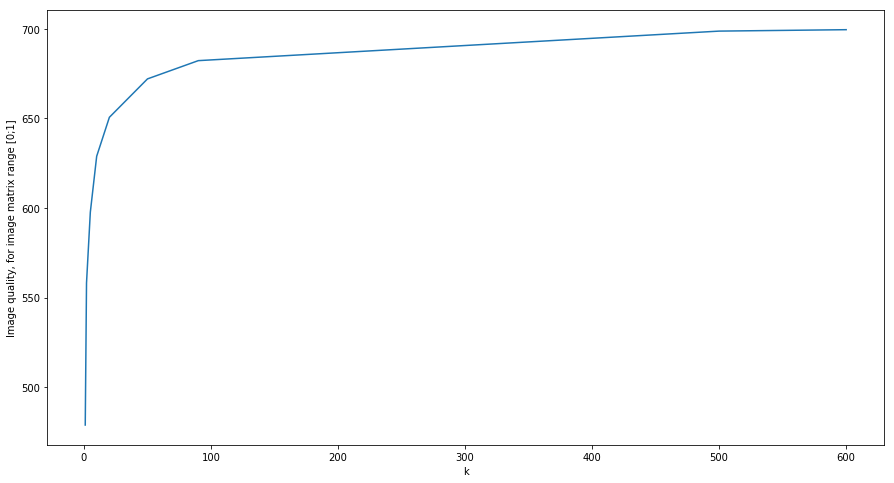
\includegraphics[width=0.56\textwidth]{ImageQuality}
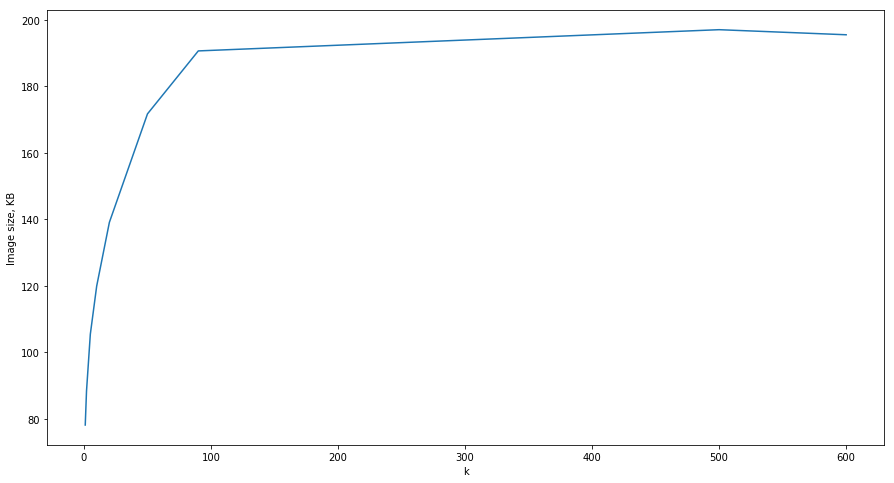
\includegraphics[width=0.56\textwidth]{ImageSize}
A person may be recognized starting from $k$ equal to 5-10 already. The quality of image increases considerably when $k$ is small, and then increasing slows down. The size increases even harder as $k$ increases until $k\approx100$, after that it doesn't change too much.\\
\end{solution}
% }


\begin{problem}[Polar decomposition; 3 pt]\label{prb:13.8}\rm
Find the positive definite square root $S = V\Sigma V^\top$ of~$A^\top A$ and its polar decomposition $A = QS$:
\[
   A = \frac1{\sqrt{10}} \begin{pmatrix}
     10 & 6 \\ 0 & 8
    \end{pmatrix}
\]
\end{problem}

% \textcolor{blue}{
\begin{solution}[] \rm .
\[
A = \frac1{\sqrt{10}}
\begin{pmatrix}
10 & 6 \\
0 & 8
\end{pmatrix}
\qquad A^\top A =
\begin{pmatrix}
10 & 6 \\
6 & 10
\end{pmatrix}
\]
\[
\lambda_1 = 16
\quad
\sigma_1 = 4
\qquad
\lambda_2 = 20 - 16 = 4
\quad
\sigma_2 = 2
\]
\[
\bv_1 = \frac1{\sqrt2}\begin{pmatrix} 1 \\ 1 \end{pmatrix}
\quad
\bu_1 = A \bv_1 / \sigma_1 = 
\frac1{8\sqrt{5}}
\begin{pmatrix} 16 \\ 8 \end{pmatrix} = 
\frac1{\sqrt{5}}
\begin{pmatrix} 2 \\ 1  \end{pmatrix}
\]
\[
\bv_2 = \frac1{\sqrt2}\begin{pmatrix} 1 \\ -1 \end{pmatrix}
\quad
\bu_2 = A \bv_2 / \sigma_2 = \frac1{4\sqrt{5}}
\begin{pmatrix} 4 \\ - 8 \end{pmatrix} = \frac1{\sqrt{5}}
\begin{pmatrix} 1 \\ - 2 \end{pmatrix}
\]
\[
S = V\Sigma V^\top
=
\frac1{\sqrt2}
\begin{pmatrix}
1 & 1 \\
1 & -1
\end{pmatrix}
\begin{pmatrix}
4 & 0 \\
0 & 2
\end{pmatrix}
\frac1{\sqrt2}
\begin{pmatrix}
1 & 1 \\
1 & -1
\end{pmatrix}
=
\frac1{2}
\begin{pmatrix}
1 & 1 \\
1 & -1
\end{pmatrix}
\begin{pmatrix}
4 & 4 \\
2 & -2
\end{pmatrix}
=
\begin{pmatrix}
3 & 1 \\
1 & 3
\end{pmatrix}
\]
\[
A = U\Sigma V^\top = UV^\top (V\Sigma V^\top) = QS
\]
\[
Q = UV^\top = 
\frac1{\sqrt5}
\begin{pmatrix}
2 & 1 \\
1 & -2
\end{pmatrix}
\frac1{\sqrt2}
\begin{pmatrix}
1 & 1 \\
1 & -1
\end{pmatrix}
=
\frac1{\sqrt{10}}
\begin{pmatrix}
3 & 1 \\
-1 & 3
\end{pmatrix}
\]
\answer{
$
S = \begin{pmatrix}
3 & 1 \\
1 & 3
\end{pmatrix};~
A = QS = 
\frac1{\sqrt{10}}
\begin{pmatrix}
3 & 1 \\
-1 & 3
\end{pmatrix}
\begin{pmatrix}
3 & 1 \\
1 & 3
\end{pmatrix}
$
}\\[5pt]
\end{solution}
% }


\begin{problem}[Pseudoinverses and shortest solutions; 5 pt]\rm
	\begin{enumerate}[(a)]
		\item Find the SVD and the pseudoinverse $V\Sigma^+U^\top$ of the matrices
		\[
		A =
		\begin{pmatrix}
			1 & 1 & 1 & 1
		\end{pmatrix},
		\qquad
		B = \begin{pmatrix}
			0 & 1 & 0 \\ 1 & 0 & 0
		\end{pmatrix},\qquad
		C =
		\begin{pmatrix}
		1 & 1 \\ 0 & 0
		\end{pmatrix}.
		\]
		\item Find the minimum-length solution $\bx^+ = A^+ \bb$ of the equation $A\bx = \bb$ with
		\[
		A =  \begin{pmatrix}[rrr]
		1 & 0 & 0 \\ 1 & 0 & 0 \\ 1 & 1 & 1
		\end{pmatrix},
		\qquad \bb = \begin{pmatrix}
		0 \\ 2 \\ 2
		\end{pmatrix}.
		\]
	\end{enumerate}
\end{problem}

% \textcolor{blue}{
\begin{solution}[] \rm
% \[
% A = U \Sigma V^\top
% \]
Let $\hat A = A^T$.
\[
\hat A = \hat U \hat\Sigma \hat V^\top
~\Rightarrow~
% A = \hat V \hat\Sigma^\top \hat U^\top \Rightarrow 
\left \{ \begin{matrix}
U = \hat V \\
\Sigma = \hat\Sigma^\top \\
V = \hat U \\
\end{matrix}\right. \text{ for } A
~\Rightarrow~
A^+ = V \Sigma^+ U^\top = \hat U \Sigma^+ \hat V^\top\\
\]
\begin{enumerate}[(a)]
	\item
\[
A =
\begin{pmatrix}
1 & 1 & 1 & 1
\end{pmatrix}
\qquad
\hat A =
\begin{pmatrix}
1 \\ 1 \\ 1 \\ 1
\end{pmatrix}
\qquad
\hat A^\top\hat A = 
\begin{pmatrix} 4 \end{pmatrix}
\]
\[
\lambda_1 = 4 \qquad \sigma_1 = 2
\qquad
\hat \Sigma = \begin{pmatrix} 2 \\ 0 \\ 0 \\ 0 \end{pmatrix}
~\Rightarrow~
\Sigma^+ = \begin{pmatrix} 1/2 \\ 0 \\ 0 \\ 0 \end{pmatrix}
\qquad
\hat \bv_1 = \begin{pmatrix} 1 \end{pmatrix}
\qquad
\hat \bu_1 = \frac{\hat A \hat \bv}{\norm{\cdot}} = \frac12 \begin{pmatrix} 1 \\ 1 \\ 1 \\ 1 \end{pmatrix}
\]
Let's complete $\hat U$ to an ONB of $\bR^4$:
\[
\hat U = \frac12
\begin{pmatrix}[rrrr]
1 & 1 & 1 & 1\\
1 & -1 & -1 & 1\\
1 & 1 & -1 & -1\\
1 & -1 & 1 & -1
\end{pmatrix}
\Rightarrow
A^+ =\frac12
\begin{pmatrix}[rrrr]
1 & 1 & 1 & 1\\
1 & -1 & -1 & 1\\
1 & 1 & -1 & -1\\
1 & -1 & 1 & -1
\end{pmatrix}
\begin{pmatrix} 1/2 \\ 0 \\ 0 \\ 0 \end{pmatrix}
= \frac14
\begin{pmatrix} 1 \\ 1 \\ 1 \\ 1 \end{pmatrix}
\]\\[10pt]
\[
B = \begin{pmatrix}
0 & 1 & 0 \\
1 & 0 & 0
\end{pmatrix}
\qquad
\hat B = \begin{pmatrix}
0 & 1 \\
1 & 0 \\
0 & 0 \\
\end{pmatrix}
\qquad
\hat B^\top \hat B = \begin{pmatrix}
1 & 0\\
0 & 1 
\end{pmatrix}
\]
\[
\lambda_1=\lambda_2=1
\qquad
\sigma_1=\sigma_2=1
\qquad
\hat\Sigma = \begin{pmatrix}
1 & 0 \\
0 & 1 \\
0 & 0 \\
\end{pmatrix}
= \Sigma^+
\]
\[
\hat \bv_1 = \begin{pmatrix} 1 \\ 0 \end{pmatrix}
\quad
\hat \bv_2 = \begin{pmatrix} 0 \\ 1 \end{pmatrix}
\qquad
\hat \bu_1 = \begin{pmatrix} 0 \\ 1 \\ 0 \end{pmatrix}
\quad
\hat \bu_2 = \begin{pmatrix} 1 \\ 0 \\ 0 \end{pmatrix}
\quad
\hat \bu_3 = \begin{pmatrix} 0 \\ 0 \\ 1 \end{pmatrix}
\]
\[
B^+ = \hat U \Sigma^+ \hat V^\top = 
\begin{pmatrix}
0 & 1 & 0 \\
1 & 0 & 0 \\
0 & 0 & 1 \\
\end{pmatrix}
\begin{pmatrix}
1 & 0 \\
0 & 1 \\
0 & 0 \\
\end{pmatrix}
\begin{pmatrix}
1 & 0 \\
0 & 1 \\
\end{pmatrix}
=
\begin{pmatrix}
0 & 1 \\
1 & 0 \\
0 & 0 \\
\end{pmatrix}
\]
\\[10pt]
\[
C =
\begin{pmatrix}
1 & 1 \\ 0 & 0
\end{pmatrix}
\hat C =
\begin{pmatrix}
1 & 0 \\ 1 & 0
\end{pmatrix}
\hat C^\top \hat C = 
\begin{pmatrix}
2 & 0 \\ 0 & 0
\end{pmatrix}
\]
\[
\lambda_1 = 2
\qquad
\sigma_1 = \sqrt2
\qquad
\hat \Sigma = 
\begin{pmatrix}
\sqrt2 & 0 \\ 0 & 0
\end{pmatrix}
~\Rightarrow~
\Sigma^+ = 
\begin{pmatrix}
1/\sqrt2 & 0 \\ 0 & 0
\end{pmatrix}
\]
\[
\qquad
\hat \bv_1 = \begin{pmatrix} 1 \\ 0 \end{pmatrix}
\quad
\hat \bv_2 = \begin{pmatrix} 0 \\ 1 \end{pmatrix}
\qquad
\hat \bu_1 = \frac1{\sqrt2}\begin{pmatrix} 1 \\ 1 \end{pmatrix}
\quad
\hat \bu_2 = \frac1{\sqrt2}\begin{pmatrix} 1 \\ -1 \end{pmatrix}
\]
\[
C^+ = \hat U \Sigma^+ \hat V^\top = 
\frac1{\sqrt2}
\begin{pmatrix}
1 & 1 \\
1 & -1 \\
\end{pmatrix}
\begin{pmatrix}
1/\sqrt2 & 0 \\
0 & 0
\end{pmatrix}
\begin{pmatrix}
1 & 0 \\
0 & 1 \\
\end{pmatrix}
= \frac12
\begin{pmatrix}
1 & 0 \\
1 & 0 \\
\end{pmatrix}
\]
\answer{$
A^+ = \frac14
\begin{pmatrix} 1 \\ 1 \\ 1 \\ 1 \end{pmatrix}
\qquad
B^+ =
\begin{pmatrix}
0 & 1 \\
1 & 0 \\
0 & 0 \\
\end{pmatrix}
\qquad
C^+ = 
\frac12
\begin{pmatrix}
1 & 0 \\
1 & 0 \\
\end{pmatrix}
$}
	\item 
\[
\bb = 
\begin{pmatrix}
0 \\ 2 \\ 2
\end{pmatrix}
\qquad
A = \begin{pmatrix}[rrr]
1 & 0 & 0 \\ 1 & 0 & 0 \\ 1 & 1 & 1
\end{pmatrix}
\qquad
\hat A = 
\begin{pmatrix}[rrr]
1 & 1 & 1 \\
0 & 0 & 1 \\
0 & 0 & 1
\end{pmatrix}
\qquad
\hat A^\top \hat A =
\begin{pmatrix}[rrr]
1 & 1 & 1 \\
1 & 1 & 1 \\
1 & 1 & 3
\end{pmatrix}
\]
\[
\lambda_1 = 4
\quad
\lambda_2 = 1
\qquad
\sigma_1 = 2
\quad
\sigma_2 = 1
\qquad
\hat \Sigma = \begin{pmatrix}
2 & 0 & 0 \\
0 & 1 & 0 \\
0 & 0 & 0
\end{pmatrix}
~\Rightarrow~
\Sigma^+ = \begin{pmatrix}
1/2 & 0 & 0 \\
0 & 1 & 0 \\
0 & 0 & 0
\end{pmatrix}
\]
\[
\begin{pmatrix}[rrr]
-3 & 1 & 1 \\
1 & -3 & 1 \\
1 & 1 & -1
\end{pmatrix}\bv = 0
\qquad
\hat \bv_1 = \frac1{\sqrt6}
\begin{pmatrix}[rrr] 
1 \\ 1 \\ 2
\end{pmatrix}
\qquad
\hat \bu_1 = \frac{
\begin{pmatrix}[rrr]
1 & 1 & 1 \\
0 & 0 & 1 \\
0 & 0 & 1
\end{pmatrix}
\begin{pmatrix}[rrr] 
1 \\ 1 \\ 2
\end{pmatrix}}{\norm{\cdot}}
= \frac1{\sqrt6}
\begin{pmatrix}[rrr] 
2 \\ 1 \\ 1
\end{pmatrix}
\]
\[
\begin{pmatrix}[rrr]
0 & 1 & 1 \\
1 & 0 & 1 \\
1 & 1 & 2
\end{pmatrix}\bv = 0
\qquad
\hat \bv_2 = \frac1{\sqrt3}
\begin{pmatrix}[rrr] 
1 \\ 1 \\ -1
\end{pmatrix}
\qquad
\hat \bu_2 = \frac{
\begin{pmatrix}[rrr]
1 & 1 & 1 \\
0 & 0 & 1 \\
0 & 0 & 1
\end{pmatrix}
\begin{pmatrix}[rrr] 
1 \\ 1 \\ -1
\end{pmatrix}}{\norm{\cdot}}
= \frac1{\sqrt3}
\begin{pmatrix}[rrr] 
1 \\ -1 \\ -1
\end{pmatrix}
\]
\[
\hat \bu_3 = \frac1{\sqrt2}
\begin{pmatrix}[rrr] 
0 \\ 1 \\ -1
\end{pmatrix} \text{ (by G-S) }
\qquad
\hat V = \frac1{\sqrt6}
\begin{pmatrix}[rrr] 
1 & \sqrt2 & \sqrt3\\
1 & \sqrt2 & -\sqrt3\\
2 & -\sqrt2 & 0\\
\end{pmatrix}
\qquad
\hat U = \frac1{\sqrt6}
\begin{pmatrix}[rrr] 
2 & \sqrt2 & 0\\
1 & -\sqrt2 & \sqrt3\\
1 & -\sqrt2 & -\sqrt3\\
\end{pmatrix}
\]
\[
A^+ = \frac16
\begin{pmatrix}[rrr] 
2 & \sqrt2 & 0\\
1 & -\sqrt2 & \sqrt3\\
1 & -\sqrt2 & -\sqrt3\\
\end{pmatrix}
\begin{pmatrix}
1/2 & 0 & 0 \\
0 & 1 & 0 \\
0 & 0 & 0
\end{pmatrix}
\begin{pmatrix}[rrr] 
1 & \sqrt2 & \sqrt3\\
1 & \sqrt2 & -\sqrt3\\
2 & -\sqrt2 & 0\\
\end{pmatrix}
= \frac14
\begin{pmatrix}[rrr] 
2 & 2 & 0 \\
-1 & -1 & 2 \\
-1 & -1 & 2 \\
\end{pmatrix}
\]
\[
\bx^+ = A^+\bb =  \frac14
\begin{pmatrix}[rrr] 
2 & 2 & 0 \\
-1 & -1 & 2 \\
-1 & -1 & 2 \\
\end{pmatrix}
\begin{pmatrix}
0 \\ 2 \\ 2
\end{pmatrix}
=
\begin{pmatrix}
1 \\ 1/2 \\ 1/2
\end{pmatrix}
\]
\answer{$
\bx^+ =
\begin{pmatrix}
1 \\ 1/2 \\ 1/2
\end{pmatrix}
$}\\[5pt]
\end{enumerate}
\end{solution}
% }


\begin{problem}[Principal component analysis; 3 pt]\label{prb:13.7}\rm
\begin{enumerate}[(a)]
  \item Convert the matrix of observation $A$ to the zero-mean form and then construct the sample covariance matrix:
  \[
    A = \begin{pmatrix}[rrrrrr]
      19 & 22 & 6 & 3 & 2 & 20\\ 12 & 6 & 9 & 15 & 13 & 5
    \end{pmatrix}
  \]  
  \item Find the principal components of the data in matrix~$A$.
  \item Let $x_1$, $x_2$ denote the variables for the two-dimensional data in (a). Find the new variable $y_1 = a_1x_1 + a_2 x_2$ such that $y_1$ has maximum possible variance over the given data. How much of the variance in the data is explained by~$y_1$?
\end{enumerate}
\end{problem}

% \textcolor{red}{
\begin{solution}[] \rm .
\begin{enumerate}[(a)]
  \item The matrix of observation A is $m\times n$, where $m=2$ is the dimensionality of the data, $n=6$ -- number of observations (columns). To convert to zero-mean form we calculate mean point across the observations and subtract it from each column of A.
\[
A = \begin{pmatrix}[rrrrrr]
19 & 22 & 6 & 3 & 2 & 20\\
12 & 6 & 9 & 15 & 13 & 5
\end{pmatrix}
\qquad
\mu = \begin{pmatrix}[rrrrrr]
12 \\ 10
\end{pmatrix}
\qquad
A_0 = \begin{pmatrix}[rrrrrr]
7 & 10 & -6 & -9 & -10 & 8 \\
2 & -4 & -1 & 5 &  3 & -5
\end{pmatrix}
\]
\[
C = A_0 A_0^\top = \begin{pmatrix}[rr]
 430 & -135 \\
-135 &   80 \\
 \end{pmatrix} ~\text{ -- ~sample covariance matrix}
\]
  \item To find the principal components we find the eigenvalues and eigenvectors of the covariance matrix.
\[
\det(C-\lambda) = \lambda^2 - 510 \lambda + 16175
\]
\[
\lambda_1 = 5\left(51+\sqrt{1954}\right) \approx 476.02
\qquad
\lambda_2 = 5\left(51-\sqrt{1954}\right) \approx 33.98
\]
\[
\begin{pmatrix}[rr]
 430-\lambda & -135 \\
-135 &   80-\lambda \\
\end{pmatrix}
\bv = 0
\]
Solving the equation for the eigenvalues $\lambda_1, \lambda_2$ we get:
\[
\bv_1 \approx \begin{pmatrix}0.95 \\-0.32\end{pmatrix}
\text{ -- the first principal component~~~~}
\]
\[
\bv_2 \approx \begin{pmatrix}0.32 \\ 0.95\end{pmatrix}
\text{ -- the second principal component}
\]
  \item The new transformed variable with maximum possible variance can be found from the first principal component:
 \[
 y_1 = \bv_1^\top \bx = 0.95 x_1 - 0.32 x_2
 \qquad
 \lambda_1 = 476.02 \text{ -- corresponds to the variance of $y_1$}
 \]
 And the fraction of the total variance is:
 \[
 \frac{\lambda_1}{\sum_{i=1}^2 \lambda_i} = 93.3\%
 \]
 So, the new transformed and restricted data would be:
 \[
Y_1 = \begin{pmatrix}[rrrrrr]
14.11 & 18.89 & 2.78 & -2 & -2.3 & 17.32
\end{pmatrix}
 \]
And, indeed:
\[
\frac{Var(Y_1)}{\sum_{i=1}^2 Var(A_i)} = \frac{79.34}{71.67+13.33} = 93.3\%
\]
, where $A_i$ corresponds to observations of the $i^{th}$ component (row) of the data.\\
\end{enumerate}
\end{solution}
% }


%\newpage

\begin{problem}[PCA; 5~pt]\label{prb:PCA}\rm
	\begin{itemize}
		\item[(a)] Simulate $N=100$ data $(x_k,y_k)$ from the two-dimensional Gaussian (normal) distribution $\mathcal{N}(\mu_1,\mu_2; \sigma_1^2,\sigma_2^2, \rho)$ with $\mu_1 = 1$, $\mu_2 = 2$, $\sigma_1 = 4$, $\sigma_2 = 9$, $\rho=\tfrac13$.
		
		\small{\textsf{Hint: Can you do this easily if $\rho = 0$? If $(Z_1,Z_2)^\top \sim \mathcal{N}(0,0; 1,1, 0)$, show that $(X,Y)^\top$ with $X = \mu_1+ \sigma_1 Z_1$ and $Y = \mu_2 + \sigma_2\rho Z_1 + \sqrt{1-\rho^2}\sigma_2Z_2$ has the required distribution}}
		
		\item[(b)] Form the empirical covariance matrix $C$ for the data simulated and find its eigenvalues and eigenvectors.
		
		\item[(c)] Perform the PCA on the data generated. Calculate the variance along the first component; what fraction of the total variance does it include?
		
		\item[(d)] Predict how the above fraction depends on $\rho$ and confirm your reasoning numerically.
	\end{itemize}
\end{problem}

% \textcolor{red}{
\begin{solution}[] \rm .
Since $Z_1, Z_2$ are normally distributed, and $X, Y$ are given from the linear transformations of $Z_1, Z_2$, it's also normally distributed. Let's find the parameters:
\[
EX = E(\mu_1 + \sigma_1 Z_1) = \mu_1
\quad
EY = E(\mu_2 + \sigma_2 \rho Z_1 + \sigma_2\sqrt{1 − \rho^2} Z_2) = \mu_2
\]
\[
Var(X) = Var(\mu_1 + \sigma_1 Z_1) = \sigma_1^2 Var(Z_1) = \sigma_1^2
\]
\[
Var(Y) = Var\left(\mu_2+\sigma_2 (\rho Z_1 + \sqrt{1 − \rho^2} Z_2)\right)
= \sigma_2^2 Var\left(\rho Z_1 + \sqrt{1 − \rho^2} Z_2\right) =
\]
\[
= \left\| \text{ $Z_1$ and $Z_2$ are independent } \right\|
= \sigma_2^2 (\rho^2 Var(Z_1) + (1 - \rho^2)Var(Z_2))
\]
\[
= \sigma_2^2  (\rho^2  + 1 - \rho^2) = \sigma_2^2 
\]
\[
Corr(X,Y) = \frac{Cov(X,Y)}{\sigma_1 \sigma_2}
= \frac{1}{\sigma_1 \sigma_2}
Cov\left(\mu_1+\sigma_1Z_1,~\mu_2+\sigma_2(\rho Z_1 + \sqrt{1 − \rho^2} Z_2)\right) =
\]
\[
= \frac{\sigma_1 \sigma_2}{\sigma_1 \sigma_2} Cov\left(Z_1,~\rho Z_1 + \sqrt{1 − \rho^2} Z_2\right)
= (\rho Var(Z_1) + \sqrt{1 − \rho^2} Cov(Z_1,  Z_2)) =
\]
\[
= \left| \text{ $Z_1$ and $Z_2$ are independent } \right|
= \rho
\]
So $(X,Y)$ has the required distribution. See the code with its output below:
    \begin{Verbatim}[commandchars=\\\{\}]
{\color{incolor}In [{\color{incolor}1}]:} \PY{k+kn}{import} \PY{n+nn}{numpy} \PY{k}{as} \PY{n+nn}{np}
        \PY{k+kn}{import} \PY{n+nn}{scipy}\PY{n+nn}{.}\PY{n+nn}{stats} \PY{k}{as} \PY{n+nn}{stats}
        \PY{k+kn}{from} \PY{n+nn}{scipy} \PY{k}{import} \PY{n}{linalg} \PY{k}{as} \PY{n}{LA}
        \PY{k+kn}{from} \PY{n+nn}{matplotlib} \PY{k}{import} \PY{n}{pyplot} \PY{k}{as} \PY{n}{plt}
        \PY{k+kn}{import} \PY{n+nn}{matplotlib} \PY{k}{as} \PY{n+nn}{mpl}
        
        \PY{k}{def} \PY{n+nf}{sample\PYZus{}mvn2D\PYZus{}from\PYZus{}1D}\PY{p}{(}\PY{n}{mu1}\PY{p}{,} \PY{n}{mu2}\PY{p}{,} \PY{n}{sigma1}\PY{p}{,} \PY{n}{sigma2}\PY{p}{,} \PY{n}{rho}\PY{p}{,} \PY{n}{N}\PY{p}{)}\PY{p}{:}
            \PY{n}{x0} \PY{o}{=} \PY{n}{np}\PY{o}{.}\PY{n}{random}\PY{o}{.}\PY{n}{normal}\PY{p}{(}\PY{n}{size}\PY{o}{=}\PY{n}{N}\PY{p}{)}
            \PY{n}{y0} \PY{o}{=} \PY{n}{np}\PY{o}{.}\PY{n}{random}\PY{o}{.}\PY{n}{normal}\PY{p}{(}\PY{n}{size}\PY{o}{=}\PY{n}{N}\PY{p}{)}
            \PY{n}{x} \PY{o}{=} \PY{n}{mu1} \PY{o}{+} \PY{n}{sigma1}\PY{o}{*}\PY{n}{x0}
            \PY{n}{y} \PY{o}{=} \PY{n}{mu2} \PY{o}{+} \PY{n}{sigma2}\PY{o}{*}\PY{p}{(}\PY{n}{rho}\PY{o}{*}\PY{n}{x0} \PY{o}{+} \PY{n}{np}\PY{o}{.}\PY{n}{sqrt}\PY{p}{(}\PY{l+m+mi}{1}\PY{o}{\PYZhy{}}\PY{n}{rho}\PY{o}{*}\PY{o}{*}\PY{l+m+mi}{2}\PY{p}{)}\PY{o}{*}\PY{n}{y0}\PY{p}{)}
            \PY{n}{A} \PY{o}{=} \PY{n}{np}\PY{o}{.}\PY{n}{hstack}\PY{p}{(}\PY{p}{(}\PY{n}{x}\PY{o}{.}\PY{n}{reshape}\PY{p}{(}\PY{o}{\PYZhy{}}\PY{l+m+mi}{1}\PY{p}{,}\PY{l+m+mi}{1}\PY{p}{)}\PY{p}{,} \PY{n}{y}\PY{o}{.}\PY{n}{reshape}\PY{p}{(}\PY{o}{\PYZhy{}}\PY{l+m+mi}{1}\PY{p}{,}\PY{l+m+mi}{1}\PY{p}{)}\PY{p}{)}\PY{p}{)}
            \PY{k}{return} \PY{n}{A}
        
        \PY{k}{def} \PY{n+nf}{visualize2D}\PY{p}{(}\PY{n}{A}\PY{p}{,} \PY{n}{cmap}\PY{o}{=}\PY{l+s+s1}{\PYZsq{}}\PY{l+s+s1}{blue}\PY{l+s+s1}{\PYZsq{}}\PY{p}{)}\PY{p}{:}
            \PY{n}{A} \PY{o}{=} \PY{n}{A}\PY{o}{.}\PY{n}{reshape}\PY{p}{(}\PY{p}{(}\PY{o}{\PYZhy{}}\PY{l+m+mi}{1}\PY{p}{,}\PY{l+m+mi}{2}\PY{p}{)}\PY{p}{)}
            \PY{n}{plt}\PY{o}{.}\PY{n}{scatter}\PY{p}{(}\PY{n}{A}\PY{p}{[}\PY{p}{:}\PY{p}{,}\PY{l+m+mi}{0}\PY{p}{]}\PY{p}{,} \PY{n}{A}\PY{p}{[}\PY{p}{:}\PY{p}{,}\PY{l+m+mi}{1}\PY{p}{]}\PY{p}{)}
            \PY{n}{lmax}\PY{p}{,} \PY{n}{lmin} \PY{o}{=} \PY{n}{np}\PY{o}{.}\PY{n}{max}\PY{p}{(}\PY{n}{A}\PY{p}{)}\PY{p}{,} \PY{n}{np}\PY{o}{.}\PY{n}{min}\PY{p}{(}\PY{n}{A}\PY{p}{)}
            \PY{n}{plt}\PY{o}{.}\PY{n}{xlim}\PY{p}{(}\PY{n}{lmin}\PY{p}{,}\PY{n}{lmax}\PY{p}{)}
            \PY{n}{plt}\PY{o}{.}\PY{n}{ylim}\PY{p}{(}\PY{n}{lmin}\PY{p}{,}\PY{n}{lmax}\PY{p}{)}
        
        \PY{k}{def} \PY{n+nf}{visualizeEVec}\PY{p}{(}\PY{n}{V}\PY{p}{)}\PY{p}{:}
            \PY{n}{V} \PY{o}{=} \PY{n}{np}\PY{o}{.}\PY{n}{array}\PY{p}{(}\PY{n}{V}\PY{p}{)}
            \PY{n}{plt}\PY{o}{.}\PY{n}{scatter}\PY{p}{(}\PY{l+m+mi}{0}\PY{p}{,}\PY{l+m+mi}{0}\PY{p}{,} \PY{n}{c}\PY{o}{=}\PY{l+s+s1}{\PYZsq{}}\PY{l+s+s1}{k}\PY{l+s+s1}{\PYZsq{}}\PY{p}{)}
            \PY{n}{plt}\PY{o}{.}\PY{n}{scatter}\PY{p}{(}\PY{n}{V}\PY{p}{[}\PY{l+m+mi}{0}\PY{p}{,}\PY{p}{:}\PY{p}{]}\PY{p}{,} \PY{n}{V}\PY{p}{[}\PY{l+m+mi}{1}\PY{p}{,}\PY{p}{:}\PY{p}{]}\PY{p}{,} \PY{n}{c}\PY{o}{=}\PY{l+s+s1}{\PYZsq{}}\PY{l+s+s1}{red}\PY{l+s+s1}{\PYZsq{}}\PY{p}{)}
        
        \PY{k}{def} \PY{n+nf}{PCA}\PY{p}{(}\PY{n}{A}\PY{p}{,} \PY{n}{out}\PY{o}{=}\PY{k+kc}{False}\PY{p}{)}\PY{p}{:}
            \PY{n}{mean\PYZus{}point} \PY{o}{=} \PY{n}{np}\PY{o}{.}\PY{n}{mean}\PY{p}{(}\PY{n}{A}\PY{p}{,} \PY{l+m+mi}{0}\PY{p}{,} \PY{n}{keepdims}\PY{o}{=}\PY{k+kc}{True}\PY{p}{)}
            \PY{n}{A0} \PY{o}{=} \PY{n}{A} \PY{o}{\PYZhy{}} \PY{n}{mean\PYZus{}point}
            \PY{n}{C} \PY{o}{=} \PY{n}{A0}\PY{o}{.}\PY{n}{T}\PY{o}{.}\PY{n}{dot}\PY{p}{(}\PY{n}{A0}\PY{p}{)}
            \PY{k}{if} \PY{n}{out}\PY{p}{:}
                \PY{n+nb}{print}\PY{p}{(}\PY{l+s+s1}{\PYZsq{}}\PY{l+s+s1}{Covariance matrix:}\PY{l+s+se}{\PYZbs{}n}\PY{l+s+si}{\PYZob{}\PYZcb{}}\PY{l+s+s1}{\PYZsq{}}\PY{o}{.}\PY{n}{format}\PY{p}{(}\PY{n}{C}\PY{p}{)}\PY{p}{)}
            \PY{n}{l}\PY{p}{,} \PY{n}{v} \PY{o}{=} \PY{n}{LA}\PY{o}{.}\PY{n}{eig}\PY{p}{(}\PY{n}{C}\PY{p}{)}
            \PY{n}{l} \PY{o}{=} \PY{n}{l}\PY{o}{.}\PY{n}{real}
            \PY{n}{ids} \PY{o}{=} \PY{n}{np}\PY{o}{.}\PY{n}{argsort}\PY{p}{(}\PY{o}{\PYZhy{}}\PY{n}{l}\PY{p}{)}
            \PY{n}{lambdas}\PY{p}{,} \PY{n}{V} \PY{o}{=} \PY{n}{l}\PY{p}{[}\PY{n}{ids}\PY{p}{]}\PY{p}{,} \PY{n}{v}\PY{p}{[}\PY{p}{:}\PY{p}{,}\PY{n}{ids}\PY{p}{]}
            \PY{n}{principal\PYZus{}components} \PY{o}{=} \PY{n+nb}{list}\PY{p}{(}\PY{n}{V}\PY{o}{.}\PY{n}{T}\PY{p}{)}
            \PY{k}{if} \PY{n}{out}\PY{p}{:}
                \PY{n+nb}{print}\PY{p}{(}\PY{l+s+s1}{\PYZsq{}}\PY{l+s+s1}{Eigenvalues \PYZam{} eigenvectors}\PY{l+s+s1}{\PYZsq{}}\PY{p}{)}
                \PY{k}{for} \PY{n}{i}\PY{p}{,} \PY{p}{(}\PY{n}{l}\PY{p}{,} \PY{n}{v}\PY{p}{)} \PY{o+ow}{in} \PY{n+nb}{enumerate}\PY{p}{(}\PY{n+nb}{list}\PY{p}{(}\PY{n+nb}{zip}\PY{p}{(}\PY{n}{lambdas}\PY{p}{,} \PY{n}{principal\PYZus{}components}\PY{p}{)}\PY{p}{)}\PY{p}{)}\PY{p}{:}
                    \PY{n+nb}{print}\PY{p}{(}\PY{l+s+s1}{\PYZsq{}}\PY{l+s+s1}{l\PYZus{}}\PY{l+s+si}{\PYZob{}\PYZcb{}}\PY{l+s+s1}{ = }\PY{l+s+si}{\PYZob{}:.2f\PYZcb{}}\PY{l+s+se}{\PYZbs{}t}\PY{l+s+s1}{v\PYZus{}}\PY{l+s+si}{\PYZob{}\PYZcb{}}\PY{l+s+s1}{ = }\PY{l+s+si}{\PYZob{}\PYZcb{}}\PY{l+s+s1}{\PYZsq{}}\PY{o}{.}\PY{n}{format}\PY{p}{(}\PY{n}{i}\PY{p}{,} \PY{n}{l}\PY{p}{,} \PY{n}{i}\PY{p}{,} \PY{n}{v}\PY{o}{.}\PY{n}{flatten}\PY{p}{(}\PY{p}{)}\PY{p}{)}\PY{p}{)}
            \PY{k}{return} \PY{n}{principal\PYZus{}components}
        
        \PY{k}{def} \PY{n+nf}{projectPoints}\PY{p}{(}\PY{n}{A}\PY{p}{,} \PY{n}{v}\PY{p}{)}\PY{p}{:}
            \PY{n}{mean\PYZus{}point} \PY{o}{=} \PY{n}{np}\PY{o}{.}\PY{n}{mean}\PY{p}{(}\PY{n}{A}\PY{p}{,} \PY{l+m+mi}{0}\PY{p}{,} \PY{n}{keepdims}\PY{o}{=}\PY{k+kc}{True}\PY{p}{)}
            \PY{n}{A0} \PY{o}{=} \PY{n}{A} \PY{o}{\PYZhy{}} \PY{n}{mean\PYZus{}point}
            \PY{n}{P} \PY{o}{=} \PY{n}{v}\PY{o}{.}\PY{n}{dot}\PY{p}{(}\PY{n}{v}\PY{o}{.}\PY{n}{T}\PY{p}{)} \PY{o}{/} \PY{p}{(}\PY{n}{v}\PY{o}{.}\PY{n}{T}\PY{o}{.}\PY{n}{dot}\PY{p}{(}\PY{n}{v}\PY{p}{)}\PY{p}{)}
            \PY{n}{PA} \PY{o}{=} \PY{p}{(}\PY{n}{P}\PY{o}{.}\PY{n}{dot}\PY{p}{(}\PY{n}{A0}\PY{o}{.}\PY{n}{T}\PY{p}{)}\PY{p}{)}\PY{o}{.}\PY{n}{T} \PY{o}{+} \PY{n}{mean\PYZus{}point}
            \PY{k}{return} \PY{n}{PA}
\end{Verbatim}

    \begin{Verbatim}[commandchars=\\\{\}]
{\color{incolor}In [{\color{incolor}2}]:} \PY{n}{N} \PY{o}{=} \PY{l+m+mi}{100}
        \PY{n}{mu1}\PY{p}{,} \PY{n}{mu2} \PY{o}{=} \PY{l+m+mi}{1}\PY{p}{,} \PY{l+m+mi}{2}
        \PY{n}{sigma1}\PY{p}{,} \PY{n}{sigma2} \PY{o}{=} \PY{l+m+mi}{4}\PY{p}{,} \PY{l+m+mi}{9}
        \PY{n}{rho} \PY{o}{=} \PY{l+m+mi}{1}\PY{o}{/}\PY{l+m+mi}{3}
        
        \PY{n}{mpl}\PY{o}{.}\PY{n}{rcParams}\PY{p}{[}\PY{l+s+s1}{\PYZsq{}}\PY{l+s+s1}{figure.figsize}\PY{l+s+s1}{\PYZsq{}}\PY{p}{]} \PY{o}{=} \PY{p}{(}\PY{l+m+mi}{5}\PY{p}{,}\PY{l+m+mi}{5}\PY{p}{)}
        \PY{n}{A} \PY{o}{=} \PY{n}{sample\PYZus{}mvn2D\PYZus{}from\PYZus{}1D}\PY{p}{(}\PY{n}{mu1}\PY{p}{,} \PY{n}{mu2}\PY{p}{,} \PY{n}{sigma1}\PY{p}{,} \PY{n}{sigma2}\PY{p}{,} \PY{n}{rho}\PY{p}{,} \PY{n}{N}\PY{p}{)}
        \PY{n}{mean\PYZus{}point} \PY{o}{=} \PY{n}{np}\PY{o}{.}\PY{n}{mean}\PY{p}{(}\PY{n}{A}\PY{p}{,} \PY{l+m+mi}{0}\PY{p}{,} \PY{n}{keepdims}\PY{o}{=}\PY{k+kc}{True}\PY{p}{)}
        \PY{n}{A0} \PY{o}{=} \PY{n}{A} \PY{o}{\PYZhy{}} \PY{n}{mean\PYZus{}point}
        \PY{n}{pc} \PY{o}{=} \PY{n}{PCA}\PY{p}{(}\PY{n}{A}\PY{p}{,} \PY{n}{out}\PY{o}{=}\PY{k+kc}{True}\PY{p}{)}
        
        \PY{n+nb}{print}\PY{p}{(}\PY{l+s+s1}{\PYZsq{}}\PY{l+s+se}{\PYZbs{}n}\PY{l+s+s1}{Centered data points (blue) with calculated principal components (red):}\PY{l+s+s1}{\PYZsq{}}\PY{p}{)}
        \PY{n}{visualize2D}\PY{p}{(}\PY{n}{A0}\PY{p}{)}
        \PY{n}{visualizeEVec}\PY{p}{(}\PY{n}{pc}\PY{p}{)}
        \PY{n}{plt}\PY{o}{.}\PY{n}{show}\PY{p}{(}\PY{p}{)}
        
        \PY{n}{v1} \PY{o}{=} \PY{n}{pc}\PY{p}{[}\PY{l+m+mi}{0}\PY{p}{]}\PY{o}{.}\PY{n}{reshape}\PY{p}{(}\PY{o}{\PYZhy{}}\PY{l+m+mi}{1}\PY{p}{,}\PY{l+m+mi}{1}\PY{p}{)}
        \PY{n}{newA} \PY{o}{=} \PY{n}{projectPoints}\PY{p}{(}\PY{n}{A}\PY{p}{,} \PY{n}{v1}\PY{p}{)}
        \PY{n}{total\PYZus{}variance} \PY{o}{=} \PY{n}{np}\PY{o}{.}\PY{n}{sum}\PY{p}{(}\PY{n}{np}\PY{o}{.}\PY{n}{var}\PY{p}{(}\PY{n}{A}\PY{p}{,} \PY{l+m+mi}{0}\PY{p}{)}\PY{p}{)}
        \PY{n}{variance1} \PY{o}{=} \PY{n}{np}\PY{o}{.}\PY{n}{mean}\PY{p}{(}\PY{n}{np}\PY{o}{.}\PY{n}{sum}\PY{p}{(}\PY{p}{(}\PY{n}{newA}\PY{o}{\PYZhy{}}\PY{n}{mean\PYZus{}point}\PY{p}{)}\PY{o}{*}\PY{o}{*}\PY{l+m+mi}{2}\PY{p}{,} \PY{n}{axis}\PY{o}{=}\PY{l+m+mi}{1}\PY{p}{)}\PY{p}{)}
        \PY{n}{fraction} \PY{o}{=} \PY{n}{variance1} \PY{o}{/} \PY{n}{total\PYZus{}variance} \PY{o}{*} \PY{l+m+mi}{100}
        \PY{n+nb}{print}\PY{p}{(}\PY{l+s+s1}{\PYZsq{}}\PY{l+s+se}{\PYZbs{}n}\PY{l+s+si}{\PYZob{}\PYZcb{}}\PY{l+s+s1}{ principal component:}\PY{l+s+s1}{\PYZsq{}}\PY{o}{.}\PY{n}{format}\PY{p}{(}\PY{l+m+mi}{1}\PY{p}{)}\PY{p}{)}
        \PY{n+nb}{print}\PY{p}{(}\PY{l+s+s1}{\PYZsq{}}\PY{l+s+se}{\PYZbs{}t}\PY{l+s+s1}{Points projected on the component (orange):}\PY{l+s+s1}{\PYZsq{}}\PY{p}{)}
        \PY{n}{visualize2D}\PY{p}{(}\PY{n}{A}\PY{p}{)}
        \PY{n}{visualize2D}\PY{p}{(}\PY{n}{newA}\PY{p}{)}
        \PY{n}{plt}\PY{o}{.}\PY{n}{show}\PY{p}{(}\PY{p}{)}
        \PY{n+nb}{print}\PY{p}{(}\PY{l+s+s1}{\PYZsq{}}\PY{l+s+se}{\PYZbs{}t}\PY{l+s+s1}{Variance along the component: }\PY{l+s+si}{\PYZob{}:.2f\PYZcb{}}\PY{l+s+s1}{\PYZsq{}}\PY{o}{.}\PY{n}{format}\PY{p}{(}\PY{n}{variance1}\PY{p}{)}\PY{p}{)}
        \PY{n+nb}{print}\PY{p}{(}\PY{l+s+s1}{\PYZsq{}}\PY{l+s+se}{\PYZbs{}t}\PY{l+s+s1}{The fration of the total variance: }\PY{l+s+si}{\PYZob{}:.2f\PYZcb{}}\PY{l+s+s1}{ / }\PY{l+s+si}{\PYZob{}:.2f\PYZcb{}}\PY{l+s+s1}{ = }\PY{l+s+si}{\PYZob{}:.2f\PYZcb{}}\PY{l+s+s1}{\PYZpc{}}\PY{l+s+s1}{\PYZsq{}}\PY{o}{.}\PY{n}{format}\PY{p}{(}\PY{n}{variance1}\PY{p}{,} \PY{n}{total\PYZus{}variance}\PY{p}{,} \PY{n}{fraction}\PY{p}{)}\PY{p}{)}
\end{Verbatim}

    \begin{Verbatim}[commandchars=\\\{\}]
Covariance matrix:
[[1675.75323616  997.42117194]
 [ 997.42117194 7602.66696436]]
Eigenvalues \& eigenvectors
l\_0 = 7766.02	v\_0 = [-0.16161994 -0.98685308]
l\_1 = 1512.40	v\_1 = [-0.98685308  0.16161994]

Centered data points (blue) with calculated principal components (red):

    \end{Verbatim}

    \begin{center}
    \adjustimage{max size={0.5\linewidth}{0.9\paperheight}}{output_1_1.png}
    \end{center}
    { \hspace*{\fill} \\}
    
    \begin{Verbatim}[commandchars=\\\{\}]

1 principal component:
	Points projected on the component (orange):

    \end{Verbatim}

    \begin{center}
    \adjustimage{max size={0.5\linewidth}{0.9\paperheight}}{output_1_3.png}
    \end{center}
    { \hspace*{\fill} \\}
    
    \begin{Verbatim}[commandchars=\\\{\}]
	Variance along the component: 77.66
	The fration of the total variance: 77.66 / 92.78 = 83.70\%

    \end{Verbatim}

    \begin{Verbatim}[commandchars=\\\{\}]
{\color{incolor}In [{\color{incolor}3}]:} \PY{n}{rhos} \PY{o}{=} \PY{n}{np}\PY{o}{.}\PY{n}{linspace}\PY{p}{(}\PY{o}{\PYZhy{}}\PY{l+m+mi}{1}\PY{p}{,}\PY{l+m+mi}{1}\PY{p}{,}\PY{l+m+mi}{50}\PY{p}{)}
        \PY{n}{fractions} \PY{o}{=} \PY{p}{[}\PY{p}{]}
        \PY{k}{for} \PY{n}{rho} \PY{o+ow}{in} \PY{n}{rhos}\PY{p}{:}
            \PY{n}{A} \PY{o}{=} \PY{n}{sample\PYZus{}mvn2D\PYZus{}from\PYZus{}1D}\PY{p}{(}\PY{n}{mu1}\PY{p}{,} \PY{n}{mu2}\PY{p}{,} \PY{n}{sigma1}\PY{p}{,} \PY{n}{sigma2}\PY{p}{,} \PY{n}{rho}\PY{p}{,} \PY{n}{N}\PY{p}{)}
            \PY{n}{mean\PYZus{}point} \PY{o}{=} \PY{n}{np}\PY{o}{.}\PY{n}{mean}\PY{p}{(}\PY{n}{A}\PY{p}{,} \PY{l+m+mi}{0}\PY{p}{,} \PY{n}{keepdims}\PY{o}{=}\PY{k+kc}{True}\PY{p}{)}
            \PY{n}{total\PYZus{}variance} \PY{o}{=} \PY{n}{np}\PY{o}{.}\PY{n}{sum}\PY{p}{(}\PY{n}{np}\PY{o}{.}\PY{n}{var}\PY{p}{(}\PY{n}{A}\PY{p}{,} \PY{l+m+mi}{0}\PY{p}{)}\PY{p}{)}
            \PY{n}{pc} \PY{o}{=} \PY{n}{PCA}\PY{p}{(}\PY{n}{A}\PY{p}{)}
            \PY{n}{v1} \PY{o}{=} \PY{n}{pc}\PY{p}{[}\PY{l+m+mi}{0}\PY{p}{]}\PY{o}{.}\PY{n}{reshape}\PY{p}{(}\PY{o}{\PYZhy{}}\PY{l+m+mi}{1}\PY{p}{,}\PY{l+m+mi}{1}\PY{p}{)}
            \PY{n}{newA} \PY{o}{=} \PY{n}{projectPoints}\PY{p}{(}\PY{n}{A}\PY{p}{,} \PY{n}{v1}\PY{p}{)}
            \PY{n}{variance1} \PY{o}{=} \PY{n}{np}\PY{o}{.}\PY{n}{mean}\PY{p}{(}\PY{n}{np}\PY{o}{.}\PY{n}{sum}\PY{p}{(}\PY{p}{(}\PY{n}{newA}\PY{o}{\PYZhy{}}\PY{n}{mean\PYZus{}point}\PY{p}{)}\PY{o}{*}\PY{o}{*}\PY{l+m+mi}{2}\PY{p}{,} \PY{n}{axis}\PY{o}{=}\PY{l+m+mi}{1}\PY{p}{)}\PY{p}{)}
            \PY{n}{fraction} \PY{o}{=} \PY{n}{variance1} \PY{o}{/} \PY{n}{total\PYZus{}variance} \PY{o}{*} \PY{l+m+mi}{100}
            \PY{n}{fractions}\PY{o}{.}\PY{n}{append}\PY{p}{(}\PY{n}{fraction}\PY{p}{)}
\end{Verbatim}

    \begin{Verbatim}[commandchars=\\\{\}]
{\color{incolor}In [{\color{incolor}4}]:} \PY{n}{mpl}\PY{o}{.}\PY{n}{rcParams}\PY{p}{[}\PY{l+s+s2}{\PYZdq{}}\PY{l+s+s2}{figure.figsize}\PY{l+s+s2}{\PYZdq{}}\PY{p}{]} \PY{o}{=} \PY{p}{(}\PY{l+m+mi}{10}\PY{p}{,}\PY{l+m+mi}{5}\PY{p}{)}
        \PY{n}{plt}\PY{o}{.}\PY{n}{plot}\PY{p}{(}\PY{n}{rhos}\PY{p}{,} \PY{n}{fractions}\PY{p}{)}
        \PY{n}{plt}\PY{o}{.}\PY{n}{xlabel}\PY{p}{(}\PY{l+s+s1}{\PYZsq{}}\PY{l+s+s1}{rho}\PY{l+s+s1}{\PYZsq{}}\PY{p}{)}
        \PY{n}{plt}\PY{o}{.}\PY{n}{ylabel}\PY{p}{(}\PY{l+s+s1}{\PYZsq{}}\PY{l+s+s1}{fraciton, }\PY{l+s+s1}{\PYZpc{}}\PY{l+s+s1}{\PYZsq{}}\PY{p}{)}
        \PY{n}{plt}\PY{o}{.}\PY{n}{show}\PY{p}{(}\PY{p}{)}
\end{Verbatim}

    \begin{center}
    \adjustimage{max size={0.9\linewidth}{0.7\paperheight}}{output_3_0.png}
    \end{center}
    { \hspace*{\fill} \\}
So, the variance fraction increases with increasing of absolute value of $\rho$.\\
\end{solution}
% }


\begin{problem}[PCA in many dimensions; 8~pt]\rm 
	This is a $10$-dimensional analogue of Problem~\ref{prb:PCA}.
	\begin{itemize}
		\item[(a)] Simulate $N=100$ data $\bx_j=(x_1^{(j)},x_2^{(j)},\dots,x_{10}^{(j)})^\top$ from the Gaussian (normal) distribution
		$\mathcal{N}(\mathbf{0},\Sigma)$ with $\Sigma = I + \bu \bu^\top$, where $\bu = (1; -2; 3; \ldots; -10)^\top$
		
		\small{\textsf{Hint: if you factorize $\Sigma = L L^\top$  with a lower-triangular~$L$ (Cholesky factorization), simulate the standard Gaussian vectors $\mathbf{z}_j = (z_1^{(j)},z_2^{(j)},\dots,z_{10}^{(j)})^\top$ (ie, with independent components of variance $1$), then $\bx = L\mathbf{z} + \bm{\mu}$ will follow $\mathcal{N}(\bm{\mu},\Sigma)$. Justify before using that!}}
		
		\item[(b)] Form the empirical covariance matrix $C$ for the data simulated and find its eigenvalues and eigenvectors.
		
		\item[(c)] Perform the PCA on the data generated. Calculate the variance along the several first component; what fraction of the total variance does it include?
		
		\item[(d)] Predict how the above fraction depends on the shape of the set $\{\bx \mid \bx^\top \Sigma \bx = 1\}$ and confirm your reasoning numerically.
		
		\small{\textsf{Hint: certainly you will need to use R, Python or MatLab libraries to solve this problem!}}
		
	\end{itemize}
\end{problem}

% \textcolor{red}{
\begin{solution}[] \rm .
Let $Z$ be a $d \times N$ data matrix ($d = 10, N=100$) generated from the standard Gaussian distribution $\mathcal N(\mathbf0_d,I_d)$. Let $\Sigma$ be a covariance matrix and $L$ -- a lower-triangular matrix from the Cholesky decomposition $\Sigma = LL^\top$, $\mu = \begin{pmatrix}\mu_1 & \cdots & \mu_d \end{pmatrix}^\top$. Since the linear transformation of the normal random variable is also a normal random variable and:
\[
X = LZ+\mu
~\Rightarrow~
EX = LE(Z)+\mu = L\b0_d+\mu = \mu
\]
\[
Var(X) = E((X - EX)(X - EX)^\top)= E(LZ (LZ)^\top) = L E(Z Z^\top)L^\top = L I_d L^\top = \Sigma
\]
we can simulate $X$ sampling using $Z$, $L$ and $\mu$: $X = LZ+\mu$.
\[
\{\bx \mid \bx^\top \Sigma \bx = 1\} = \{\bx \mid (L^\top\bx)^\top L^\top \bx = 1\} = \{\bx = L^{-\top}\by \mid \norm{\by} = 1\}
\]
Intuitively it seems that for the first principal components the fraction of the total variance will be more with such covariance matrix that skews the unit ball.
We can look at the projections of some points of the set in 2D using $\by$ (such that $\by$ has only 2 non-zero coordinates). See the code with the output below:
    \begin{Verbatim}[commandchars=\\\{\}]
{\color{incolor}In [{\color{incolor}1}]:} \PY{k+kn}{import} \PY{n+nn}{numpy} \PY{k}{as} \PY{n+nn}{np}
        \PY{k+kn}{import} \PY{n+nn}{scipy}\PY{n+nn}{.}\PY{n+nn}{stats} \PY{k}{as} \PY{n+nn}{stats}
        \PY{k+kn}{from} \PY{n+nn}{scipy} \PY{k}{import} \PY{n}{linalg} \PY{k}{as} \PY{n}{LA}
        \PY{k+kn}{from} \PY{n+nn}{matplotlib} \PY{k}{import} \PY{n}{pyplot} \PY{k}{as} \PY{n}{plt}
        \PY{k+kn}{import} \PY{n+nn}{matplotlib} \PY{k}{as} \PY{n+nn}{mpl}
        
        
        \PY{k}{def} \PY{n+nf}{sample\PYZus{}mvn\PYZus{}from1D}\PY{p}{(}\PY{n}{Mu}\PY{p}{,} \PY{n}{Sigma}\PY{p}{,} \PY{n}{N}\PY{p}{)}\PY{p}{:}
            \PY{n}{d} \PY{o}{=} \PY{n}{Sigma}\PY{o}{.}\PY{n}{shape}\PY{p}{[}\PY{l+m+mi}{0}\PY{p}{]}
            \PY{n}{Z} \PY{o}{=} \PY{n}{np}\PY{o}{.}\PY{n}{random}\PY{o}{.}\PY{n}{normal}\PY{p}{(}\PY{n}{size}\PY{o}{=}\PY{p}{(}\PY{n}{N}\PY{p}{,}\PY{n}{d}\PY{p}{)}\PY{p}{)}
            \PY{n}{L} \PY{o}{=} \PY{n}{LA}\PY{o}{.}\PY{n}{cholesky}\PY{p}{(}\PY{n}{Sigma}\PY{p}{,} \PY{n}{lower}\PY{o}{=}\PY{k+kc}{True}\PY{p}{)}
            \PY{n}{X} \PY{o}{=} \PY{n}{L}\PY{o}{.}\PY{n}{dot}\PY{p}{(}\PY{n}{Z}\PY{o}{.}\PY{n}{T}\PY{p}{)}\PY{o}{.}\PY{n}{T} \PY{o}{+} \PY{n}{Mu}
            \PY{k}{return} \PY{n}{X}
        
        \PY{k}{def} \PY{n+nf}{variance\PYZus{}along\PYZus{}axis}\PY{p}{(}\PY{n}{A}\PY{p}{,} \PY{n}{v}\PY{p}{)}\PY{p}{:}
            \PY{n}{mean\PYZus{}point} \PY{o}{=} \PY{n}{np}\PY{o}{.}\PY{n}{mean}\PY{p}{(}\PY{n}{A}\PY{p}{,} \PY{l+m+mi}{0}\PY{p}{,} \PY{n}{keepdims}\PY{o}{=}\PY{k+kc}{True}\PY{p}{)}
            \PY{n}{A\PYZus{}norm} \PY{o}{=} \PY{n}{A} \PY{o}{\PYZhy{}} \PY{n}{mean\PYZus{}point}
            \PY{n}{P} \PY{o}{=} \PY{n}{v}\PY{o}{.}\PY{n}{dot}\PY{p}{(}\PY{n}{v}\PY{o}{.}\PY{n}{T}\PY{p}{)} \PY{o}{/} \PY{p}{(}\PY{n}{v}\PY{o}{.}\PY{n}{T}\PY{o}{.}\PY{n}{dot}\PY{p}{(}\PY{n}{v}\PY{p}{)}\PY{p}{)}
            \PY{n}{PA} \PY{o}{=} \PY{p}{(}\PY{n}{P}\PY{o}{.}\PY{n}{dot}\PY{p}{(}\PY{n}{A\PYZus{}norm}\PY{o}{.}\PY{n}{T}\PY{p}{)}\PY{p}{)}\PY{o}{.}\PY{n}{T}
            \PY{n}{var} \PY{o}{=} \PY{n}{np}\PY{o}{.}\PY{n}{mean}\PY{p}{(}\PY{n}{np}\PY{o}{.}\PY{n}{sum}\PY{p}{(}\PY{n}{PA}\PY{o}{*}\PY{o}{*}\PY{l+m+mi}{2}\PY{p}{,} \PY{n}{axis}\PY{o}{=}\PY{l+m+mi}{1}\PY{p}{)}\PY{p}{)}
            \PY{k}{return} \PY{n}{var}
        
        \PY{k}{def} \PY{n+nf}{PCA}\PY{p}{(}\PY{n}{A}\PY{p}{,} \PY{n}{n\PYZus{}components}\PY{p}{,} \PY{n}{out}\PY{o}{=}\PY{k+kc}{False}\PY{p}{)}\PY{p}{:}
            \PY{n}{mean\PYZus{}point} \PY{o}{=} \PY{n}{np}\PY{o}{.}\PY{n}{mean}\PY{p}{(}\PY{n}{A}\PY{p}{,} \PY{l+m+mi}{0}\PY{p}{,} \PY{n}{keepdims}\PY{o}{=}\PY{k+kc}{True}\PY{p}{)}
            \PY{n}{A0} \PY{o}{=} \PY{n}{A} \PY{o}{\PYZhy{}} \PY{n}{mean\PYZus{}point}
            \PY{n}{C} \PY{o}{=} \PY{n}{A0}\PY{o}{.}\PY{n}{T}\PY{o}{.}\PY{n}{dot}\PY{p}{(}\PY{n}{A0}\PY{p}{)}
            \PY{k}{if} \PY{n}{out}\PY{p}{:}
                \PY{n+nb}{print}\PY{p}{(}\PY{l+s+s1}{\PYZsq{}}\PY{l+s+s1}{Covariance matrix:}\PY{l+s+se}{\PYZbs{}n}\PY{l+s+si}{\PYZob{}\PYZcb{}}\PY{l+s+s1}{\PYZsq{}}\PY{o}{.}\PY{n}{format}\PY{p}{(}\PY{n}{C}\PY{p}{)}\PY{p}{)}
            \PY{n}{l}\PY{p}{,} \PY{n}{v} \PY{o}{=} \PY{n}{LA}\PY{o}{.}\PY{n}{eig}\PY{p}{(}\PY{n}{C}\PY{p}{)}
            \PY{n}{l} \PY{o}{=} \PY{n}{l}\PY{o}{.}\PY{n}{real}
            \PY{n}{ids} \PY{o}{=} \PY{n}{np}\PY{o}{.}\PY{n}{argsort}\PY{p}{(}\PY{o}{\PYZhy{}}\PY{n}{l}\PY{p}{)}
            \PY{n}{lambdas}\PY{p}{,} \PY{n}{principal\PYZus{}components} \PY{o}{=} \PY{n}{l}\PY{p}{[}\PY{n}{ids}\PY{p}{]}\PY{p}{,} \PY{n}{v}\PY{p}{[}\PY{p}{:}\PY{p}{,}\PY{n}{ids}\PY{p}{]}
            \PY{k}{if} \PY{n}{out}\PY{p}{:}
                \PY{n+nb}{print}\PY{p}{(}\PY{l+s+s1}{\PYZsq{}}\PY{l+s+se}{\PYZbs{}n}\PY{l+s+s1}{Eigenvalues \PYZam{} eigenvectors:}\PY{l+s+s1}{\PYZsq{}}\PY{o}{.}\PY{n}{format}\PY{p}{(}\PY{n}{n\PYZus{}components}\PY{p}{)}\PY{p}{)}
                \PY{k}{for} \PY{n}{i}\PY{p}{,} \PY{p}{(}\PY{n}{l}\PY{p}{,} \PY{n}{v}\PY{p}{)} \PY{o+ow}{in} \PY{n+nb}{enumerate}\PY{p}{(}\PY{n+nb}{list}\PY{p}{(}\PY{n+nb}{zip}\PY{p}{(}\PY{n}{lambdas}\PY{p}{,} \PY{n}{principal\PYZus{}components}\PY{p}{)}\PY{p}{)}\PY{p}{)}\PY{p}{:}
                    \PY{n+nb}{print}\PY{p}{(}\PY{l+s+s1}{\PYZsq{}}\PY{l+s+s1}{l\PYZus{}}\PY{l+s+si}{\PYZob{}\PYZcb{}}\PY{l+s+s1}{ = }\PY{l+s+si}{\PYZob{}:.2f\PYZcb{}}\PY{l+s+se}{\PYZbs{}t}\PY{l+s+s1}{v\PYZus{}}\PY{l+s+si}{\PYZob{}\PYZcb{}}\PY{l+s+s1}{ = }\PY{l+s+si}{\PYZob{}\PYZcb{}}\PY{l+s+s1}{\PYZsq{}}\PY{o}{.}\PY{n}{format}\PY{p}{(}\PY{n}{i}\PY{p}{,} \PY{n}{l}\PY{p}{,} \PY{n}{i}\PY{p}{,} \PY{n}{v}\PY{o}{.}\PY{n}{flatten}\PY{p}{(}\PY{p}{)}\PY{p}{)}\PY{p}{)}
            \PY{k}{return} \PY{n}{principal\PYZus{}components}\PY{p}{[}\PY{p}{:}\PY{p}{,}\PY{p}{:}\PY{n}{n\PYZus{}components}\PY{p}{]}
        
        \PY{k}{def} \PY{n+nf}{visualize\PYZus{}set}\PY{p}{(}\PY{n}{Sigma}\PY{p}{)}\PY{p}{:}
            \PY{n+nb}{print}\PY{p}{(}\PY{l+s+s1}{\PYZsq{}}\PY{l+s+s1}{Visualization of the projections of some points }\PY{l+s+se}{\PYZbs{}n}\PY{l+s+se}{\PYZbs{}}
        \PY{l+s+s1}{of the set }\PY{l+s+s1}{\PYZob{}}\PY{l+s+s1}{x | (L\PYZca{}T x)\PYZca{}T L\PYZca{}T x = 1\PYZcb{}.}\PY{l+s+s1}{\PYZsq{}}\PY{p}{)}
            \PY{n+nb}{print}\PY{p}{(}\PY{l+s+s1}{\PYZsq{}}\PY{l+s+s1}{Different colors correspond to different (2x2) parts of L:}\PY{l+s+s1}{\PYZsq{}}\PY{p}{)}
            \PY{n}{LT} \PY{o}{=} \PY{n}{LA}\PY{o}{.}\PY{n}{cholesky}\PY{p}{(}\PY{n}{Sigma}\PY{p}{,} \PY{n}{lower}\PY{o}{=}\PY{k+kc}{True}\PY{p}{)}\PY{o}{.}\PY{n}{T}
            \PY{n}{LTinv} \PY{o}{=} \PY{n}{LA}\PY{o}{.}\PY{n}{inv}\PY{p}{(}\PY{n}{LT}\PY{p}{)}
            \PY{n}{N} \PY{o}{=} \PY{l+m+mi}{1000}
            \PY{n}{xs} \PY{o}{=} \PY{p}{(}\PY{n}{np}\PY{o}{.}\PY{n}{random}\PY{o}{.}\PY{n}{rand}\PY{p}{(}\PY{n}{N}\PY{o}{/}\PY{o}{/}\PY{l+m+mi}{2}\PY{p}{,}\PY{l+m+mi}{1}\PY{p}{)} \PY{o}{\PYZhy{}} \PY{o}{.}\PY{l+m+mi}{5}\PY{p}{)} \PY{o}{*} \PY{l+m+mi}{2}
            \PY{n}{xs} \PY{o}{=} \PY{n}{np}\PY{o}{.}\PY{n}{vstack}\PY{p}{(}\PY{p}{(}\PY{n}{xs}\PY{p}{,} \PY{p}{(}\PY{l+m+mi}{1}\PY{o}{\PYZhy{}}\PY{n}{np}\PY{o}{.}\PY{n}{random}\PY{o}{.}\PY{n}{rand}\PY{p}{(}\PY{n}{N}\PY{o}{/}\PY{o}{/}\PY{l+m+mi}{2}\PY{p}{,}\PY{l+m+mi}{1}\PY{p}{)} \PY{o}{\PYZhy{}} \PY{o}{.}\PY{l+m+mi}{5}\PY{p}{)} \PY{o}{*} \PY{l+m+mi}{2}\PY{p}{)}\PY{p}{)}
            \PY{n}{ys} \PY{o}{=} \PY{n}{np}\PY{o}{.}\PY{n}{sign}\PY{p}{(}\PY{p}{(}\PY{n}{np}\PY{o}{.}\PY{n}{random}\PY{o}{.}\PY{n}{rand}\PY{p}{(}\PY{n}{N}\PY{p}{,}\PY{l+m+mi}{1}\PY{p}{)} \PY{o}{\PYZhy{}} \PY{o}{.}\PY{l+m+mi}{5}\PY{p}{)} \PY{o}{*} \PY{l+m+mi}{2}\PY{p}{)} \PY{o}{*} \PY{n}{np}\PY{o}{.}\PY{n}{sqrt}\PY{p}{(}\PY{l+m+mi}{1} \PY{o}{\PYZhy{}} \PY{n}{xs}\PY{o}{*}\PY{o}{*}\PY{l+m+mi}{2}\PY{p}{)}
            \PY{n}{Y} \PY{o}{=} \PY{n}{np}\PY{o}{.}\PY{n}{hstack}\PY{p}{(}\PY{p}{(}\PY{n}{xs}\PY{p}{,}\PY{n}{ys}\PY{p}{)}\PY{p}{)}
            \PY{n}{lmax}\PY{p}{,} \PY{n}{lmin} \PY{o}{=} \PY{l+m+mi}{0}\PY{p}{,} \PY{l+m+mi}{0}
            \PY{k}{for} \PY{n}{i} \PY{o+ow}{in} \PY{n+nb}{range}\PY{p}{(}\PY{n}{LT}\PY{o}{.}\PY{n}{shape}\PY{p}{[}\PY{l+m+mi}{0}\PY{p}{]}\PY{o}{\PYZhy{}}\PY{l+m+mi}{1}\PY{p}{)}\PY{p}{:}
                \PY{n}{X} \PY{o}{=} \PY{p}{(}\PY{n}{LTinv}\PY{p}{[}\PY{n}{i}\PY{p}{:}\PY{n}{i}\PY{o}{+}\PY{l+m+mi}{2}\PY{p}{,}\PY{n}{i}\PY{p}{:}\PY{n}{i}\PY{o}{+}\PY{l+m+mi}{2}\PY{p}{]}\PY{o}{.}\PY{n}{dot}\PY{p}{(}\PY{n}{Y}\PY{o}{.}\PY{n}{T}\PY{p}{)}\PY{p}{)}\PY{o}{.}\PY{n}{T}
                \PY{n}{visualize2D}\PY{p}{(}\PY{n}{X}\PY{p}{)}
                \PY{n}{lmax}\PY{p}{,} \PY{n}{lmin} \PY{o}{=} \PY{n+nb}{max}\PY{p}{(}\PY{n}{np}\PY{o}{.}\PY{n}{max}\PY{p}{(}\PY{n}{X}\PY{p}{)}\PY{p}{,} \PY{n}{lmax}\PY{p}{)}\PY{p}{,} \PY{n+nb}{min}\PY{p}{(}\PY{n}{np}\PY{o}{.}\PY{n}{min}\PY{p}{(}\PY{n}{X}\PY{p}{)}\PY{p}{,} \PY{n}{lmin}\PY{p}{)}
                \PY{n}{plt}\PY{o}{.}\PY{n}{xlim}\PY{p}{(}\PY{n}{lmin}\PY{p}{,}\PY{n}{lmax}\PY{p}{)}
                \PY{n}{plt}\PY{o}{.}\PY{n}{ylim}\PY{p}{(}\PY{n}{lmin}\PY{p}{,}\PY{n}{lmax}\PY{p}{)}
            
        \PY{k}{def} \PY{n+nf}{visualize2D}\PY{p}{(}\PY{n}{A}\PY{p}{,} \PY{n}{cmap}\PY{o}{=}\PY{l+s+s1}{\PYZsq{}}\PY{l+s+s1}{blue}\PY{l+s+s1}{\PYZsq{}}\PY{p}{)}\PY{p}{:}
            \PY{n}{A} \PY{o}{=} \PY{n}{A}\PY{o}{.}\PY{n}{reshape}\PY{p}{(}\PY{p}{(}\PY{o}{\PYZhy{}}\PY{l+m+mi}{1}\PY{p}{,}\PY{l+m+mi}{2}\PY{p}{)}\PY{p}{)}
            \PY{n}{plt}\PY{o}{.}\PY{n}{scatter}\PY{p}{(}\PY{n}{A}\PY{p}{[}\PY{p}{:}\PY{p}{,}\PY{l+m+mi}{0}\PY{p}{]}\PY{p}{,} \PY{n}{A}\PY{p}{[}\PY{p}{:}\PY{p}{,}\PY{l+m+mi}{1}\PY{p}{]}\PY{p}{)}
            \PY{n}{lmax}\PY{p}{,} \PY{n}{lmin} \PY{o}{=} \PY{n}{np}\PY{o}{.}\PY{n}{max}\PY{p}{(}\PY{n}{A}\PY{p}{)}\PY{p}{,} \PY{n}{np}\PY{o}{.}\PY{n}{min}\PY{p}{(}\PY{n}{A}\PY{p}{)}
            \PY{n}{plt}\PY{o}{.}\PY{n}{xlim}\PY{p}{(}\PY{n}{lmin}\PY{p}{,}\PY{n}{lmax}\PY{p}{)}
            \PY{n}{plt}\PY{o}{.}\PY{n}{ylim}\PY{p}{(}\PY{n}{lmin}\PY{p}{,}\PY{n}{lmax}\PY{p}{)}
\end{Verbatim}

    \begin{Verbatim}[commandchars=\\\{\}]
{\color{incolor}In [{\color{incolor}2}]:} \PY{n}{mpl}\PY{o}{.}\PY{n}{rcParams}\PY{p}{[}\PY{l+s+s1}{\PYZsq{}}\PY{l+s+s1}{figure.figsize}\PY{l+s+s1}{\PYZsq{}}\PY{p}{]} \PY{o}{=} \PY{p}{(}\PY{l+m+mi}{5}\PY{p}{,}\PY{l+m+mi}{5}\PY{p}{)}
        \PY{n}{N} \PY{o}{=} \PY{l+m+mi}{100}
        \PY{n}{d} \PY{o}{=} \PY{l+m+mi}{10}
        \PY{n}{Mu} \PY{o}{=} \PY{n}{np}\PY{o}{.}\PY{n}{zeros}\PY{p}{(}\PY{n}{d}\PY{p}{)}
        \PY{n}{u} \PY{o}{=} \PY{n}{np}\PY{o}{.}\PY{n}{array}\PY{p}{(}\PY{p}{[}\PY{p}{(}\PY{o}{\PYZhy{}}\PY{l+m+mi}{1}\PY{p}{)}\PY{o}{*}\PY{o}{*}\PY{n}{i}\PY{o}{*}\PY{p}{(}\PY{n}{i}\PY{o}{+}\PY{l+m+mi}{1}\PY{p}{)} \PY{k}{for} \PY{n}{i} \PY{o+ow}{in} \PY{n+nb}{range}\PY{p}{(}\PY{l+m+mi}{10}\PY{p}{)}\PY{p}{]}\PY{p}{)}\PY{o}{.}\PY{n}{reshape}\PY{p}{(}\PY{o}{\PYZhy{}}\PY{l+m+mi}{1}\PY{p}{,}\PY{l+m+mi}{1}\PY{p}{)}
        \PY{n}{Sigma} \PY{o}{=} \PY{n}{np}\PY{o}{.}\PY{n}{eye}\PY{p}{(}\PY{n}{d}\PY{p}{)}\PY{o}{+}\PY{n}{u}\PY{o}{.}\PY{n}{dot}\PY{p}{(}\PY{n}{u}\PY{o}{.}\PY{n}{T}\PY{p}{)}
        \PY{n}{visualize\PYZus{}set}\PY{p}{(}\PY{n}{Sigma}\PY{p}{)}
        \PY{n}{plt}\PY{o}{.}\PY{n}{show}\PY{p}{(}\PY{p}{)}
        \PY{n}{A} \PY{o}{=} \PY{n}{sample\PYZus{}mvn\PYZus{}from1D}\PY{p}{(}\PY{n}{Mu}\PY{p}{,} \PY{n}{Sigma}\PY{p}{,} \PY{n}{N}\PY{p}{)}
        \PY{n}{n\PYZus{}components} \PY{o}{=} \PY{l+m+mi}{5}
        \PY{n}{total\PYZus{}variance} \PY{o}{=} \PY{n}{np}\PY{o}{.}\PY{n}{sum}\PY{p}{(}\PY{n}{np}\PY{o}{.}\PY{n}{var}\PY{p}{(}\PY{n}{A}\PY{p}{,} \PY{l+m+mi}{0}\PY{p}{)}\PY{p}{)}
        \PY{n}{pc} \PY{o}{=} \PY{n}{PCA}\PY{p}{(}\PY{n}{A}\PY{p}{,} \PY{n}{n\PYZus{}components}\PY{p}{,} \PY{n}{out}\PY{o}{=}\PY{k+kc}{True}\PY{p}{)}
        \PY{n+nb}{print}\PY{p}{(}\PY{p}{)}
        \PY{k}{for} \PY{n}{i} \PY{o+ow}{in} \PY{n+nb}{range}\PY{p}{(}\PY{n}{n\PYZus{}components}\PY{p}{)}\PY{p}{:}
            \PY{n}{v} \PY{o}{=} \PY{n}{pc}\PY{p}{[}\PY{p}{:}\PY{p}{,}\PY{n}{i}\PY{p}{]}\PY{o}{.}\PY{n}{reshape}\PY{p}{(}\PY{o}{\PYZhy{}}\PY{l+m+mi}{1}\PY{p}{,}\PY{l+m+mi}{1}\PY{p}{)}
            \PY{n}{variance} \PY{o}{=} \PY{n}{variance\PYZus{}along\PYZus{}axis}\PY{p}{(}\PY{n}{A}\PY{p}{,} \PY{n}{v}\PY{p}{)}
            \PY{n}{fraction} \PY{o}{=} \PY{n}{variance} \PY{o}{/} \PY{n}{total\PYZus{}variance} \PY{o}{*} \PY{l+m+mi}{100}
            \PY{n+nb}{print}\PY{p}{(}\PY{l+s+s1}{\PYZsq{}}\PY{l+s+si}{\PYZob{}\PYZcb{}}\PY{l+s+s1}{ principal component:}\PY{l+s+s1}{\PYZsq{}}\PY{o}{.}\PY{n}{format}\PY{p}{(}\PY{n}{i}\PY{o}{+}\PY{l+m+mi}{1}\PY{p}{,} \PY{n}{v}\PY{o}{.}\PY{n}{flatten}\PY{p}{(}\PY{p}{)}\PY{p}{)}\PY{p}{)}
            \PY{n+nb}{print}\PY{p}{(}\PY{l+s+s1}{\PYZsq{}}\PY{l+s+se}{\PYZbs{}t}\PY{l+s+s1}{Variance along the component: }\PY{l+s+si}{\PYZob{}:.2f\PYZcb{}}\PY{l+s+s1}{\PYZsq{}}\PY{o}{.}\PY{n}{format}\PY{p}{(}\PY{n}{variance}\PY{p}{)}\PY{p}{)}
            \PY{n+nb}{print}\PY{p}{(}\PY{l+s+s1}{\PYZsq{}}\PY{l+s+se}{\PYZbs{}t}\PY{l+s+s1}{The fraction of the total variance: }\PY{l+s+si}{\PYZob{}:.2f\PYZcb{}}\PY{l+s+s1}{ / }\PY{l+s+si}{\PYZob{}:.2f\PYZcb{}}\PY{l+s+s1}{ = }\PY{l+s+si}{\PYZob{}:.2f\PYZcb{}}\PY{l+s+s1}{\PYZpc{}}\PY{l+s+s1}{\PYZsq{}}\PY{o}{.}\PY{n}{format}\PY{p}{(}\PY{n}{variance}\PY{p}{,} \PY{n}{total\PYZus{}variance}\PY{p}{,} \PY{n}{fraction}\PY{p}{)}\PY{p}{)}
\end{Verbatim}

    \begin{Verbatim}[commandchars=\\\{\}]
Visualization of the projections of some points 
of the set \{x | (L\^{}T x)\^{}T L\^{}T x = 1\}.
Different colors correspond to different (2x2) parts of L:

    \end{Verbatim}

    \begin{center}
    \adjustimage{max size={0.5\linewidth}{0.9\paperheight}}{12output_1_1.png}
    \end{center}
    { \hspace*{\fill} \\}
    
    \begin{Verbatim}[commandchars=\\\{\}]
Covariance matrix:
[[  214.78971657  -201.24955179   300.72160209  -385.72372796
    529.6520468   -611.37256151   705.68227067  -785.75569745
    868.94607174  -991.48615739]
 [ -201.24955179   537.03948453  -657.00300317   820.12962187
  -1089.48325768  1274.24170173 -1454.40059324  1647.7134575
  -1849.45677325  2036.21055661]
 [  300.72160209  -657.00300317  1076.20879342 -1180.01687008
   1598.14637295 -1870.08046825  2176.96746085 -2470.6720384
   2749.01159692 -3057.06573498]
 [ -385.72372796   820.12962187 -1180.01687008  1607.81048663
  -2000.03664061  2361.37559348 -2731.42892245  3069.48603077
  -3451.32196591  3853.66346444]
 [  529.6520468  -1089.48325768  1598.14637295 -2000.03664061
   2767.26495399 -3141.47549752  3655.56988208 -4090.77292491
   4620.36946533 -5128.81104216]
 [ -611.37256151  1274.24170173 -1870.08046825  2361.37559348
  -3141.47549752  3791.3181555  -4296.12885672  4837.60632513
  -5445.56903835  6042.94906325]
 [  705.68227067 -1454.40059324  2176.96746085 -2731.42892245
   3655.56988208 -4296.12885672  5057.15912953 -5602.80979281
   6303.60656621 -6994.7646079 ]
 [ -785.75569745  1647.7134575  -2470.6720384   3069.48603077
  -4090.77292491  4837.60632513 -5602.80979281  6400.591782
  -7063.53973294  7869.54292829]
 [  868.94607174 -1849.45677325  2749.01159692 -3451.32196591
   4620.36946533 -5445.56903835  6303.60656621 -7063.53973294
   8075.30042715 -8865.16181702]
 [ -991.48615739  2036.21055661 -3057.06573498  3853.66346444
  -5128.81104216  6042.94906325 -6994.7646079   7869.54292829
  -8865.16181702  9968.56548489]]

Eigenvalues \& eigenvectors:
l\_0 = 38553.62	v\_0 = [ 0.05069188  0.10630869  0.25196444 -0.71117634  0.36112074 
                         0.0940609  0.26835339 -0.32456015 -0.25349071 -0.18974959]
l\_1 = 158.97	v\_1 = [-0.10576754  0.39091391 -0.58590637 -0.14809867  0.16127227 
                         0.17173819 -0.23807858 -0.21036262 -0.12280814  0.5470481 ]
l\_2 = 134.95	v\_2 = [ 0.15746259 -0.65532099 -0.25118828 -0.00585876  0.15823129 
                        -0.44684209  0.07969758 -0.44932539  0.09009407  0.20387032]
l\_3 = 134.29	v\_3 = [-0.19755108 -0.14206053 -0.41570398  0.09890565  0.60579719 
                         0.16523503  0.33971232  0.39989432  0.16673445 -0.24655041]
l\_4 = 121.58	v\_4 = [ 0.26361037 -0.05062176  0.38540734 -0.06938088  0.46176641 
                        -0.21528201 -0.28926165  0.47068041 -0.06146408  0.453905  ]
l\_5 = 107.77	v\_5 = [-0.31053846 -0.01581623 -0.154455   -0.0314059   0.1211     
                        -0.39028824 -0.57065775  0.03795466 -0.41308429 -0.4623348 ]
l\_6 = 89.88	v\_6 = [ 0.3596452  -0.018248   -0.00080067 -0.02997386  0.21191232 
                         0.33795537 -0.53581496 -0.23252026  0.52900921 -0.29881183]
l\_7 = 77.20	v\_7 = [-0.40447002  0.42244607  0.28522643  0.24999423  0.28817262 
                        -0.38844971  0.09066107 -0.31512673  0.41344372  0.04117586]
l\_8 = 63.05	v\_8 = [ 0.45525776  0.20228606  0.02466264  0.59015555  0.27238072 
                         0.07480811  0.1359388  -0.26071837 -0.47121571 -0.12101123]
l\_9 = 54.75	v\_9 = [-0.50625863 -0.40463804  0.32088023  0.21213012  0.14669942 
                         0.51508598 -0.16257261 -0.21041461 -0.19363921  0.19228197]

1 principal component:
	Variance along the component: 385.54
	The fraction of the total variance: 385.54 / 394.96 = 97.61\%
2 principal component:
	Variance along the component: 1.59
	The fraction of the total variance: 1.59 / 394.96 = 0.40\%
3 principal component:
	Variance along the component: 1.35
	The fraction of the total variance: 1.35 / 394.96 = 0.34\%
4 principal component:
	Variance along the component: 1.34
	The fraction of the total variance: 1.34 / 394.96 = 0.34\%
5 principal component:
	Variance along the component: 1.22
	The fraction of the total variance: 1.22 / 394.96 = 0.31\%

    \end{Verbatim}

    \begin{Verbatim}[commandchars=\\\{\}]
{\color{incolor}In [{\color{incolor}3}]:} \PY{n}{mpl}\PY{o}{.}\PY{n}{rcParams}\PY{p}{[}\PY{l+s+s1}{\PYZsq{}}\PY{l+s+s1}{figure.figsize}\PY{l+s+s1}{\PYZsq{}}\PY{p}{]} \PY{o}{=} \PY{p}{(}\PY{l+m+mi}{5}\PY{p}{,}\PY{l+m+mi}{5}\PY{p}{)}
        \PY{n}{N} \PY{o}{=} \PY{l+m+mi}{100}
        \PY{n}{d} \PY{o}{=} \PY{l+m+mi}{10}
        \PY{n}{Mu} \PY{o}{=} \PY{n}{np}\PY{o}{.}\PY{n}{zeros}\PY{p}{(}\PY{n}{d}\PY{p}{)}
        \PY{n}{u} \PY{o}{=} \PY{n}{np}\PY{o}{.}\PY{n}{array}\PY{p}{(}\PY{p}{[}\PY{p}{(}\PY{o}{\PYZhy{}}\PY{l+m+mi}{1}\PY{p}{)}\PY{o}{*}\PY{o}{*}\PY{n}{i}\PY{o}{*}\PY{p}{(}\PY{n}{i}\PY{o}{+}\PY{l+m+mi}{1}\PY{p}{)} \PY{k}{for} \PY{n}{i} \PY{o+ow}{in} \PY{n+nb}{range}\PY{p}{(}\PY{l+m+mi}{10}\PY{p}{)}\PY{p}{]}\PY{p}{)}\PY{o}{.}\PY{n}{reshape}\PY{p}{(}\PY{o}{\PYZhy{}}\PY{l+m+mi}{1}\PY{p}{,}\PY{l+m+mi}{1}\PY{p}{)}
        \PY{n}{Sigma} \PY{o}{=} \PY{n}{np}\PY{o}{.}\PY{n}{eye}\PY{p}{(}\PY{n}{d}\PY{p}{)}\PY{o}{+}\PY{n}{u}\PY{o}{.}\PY{n}{dot}\PY{p}{(}\PY{n}{u}\PY{o}{.}\PY{n}{T}\PY{p}{)} \PY{o}{/} \PY{l+m+mi}{100}
        \PY{n}{visualize\PYZus{}set}\PY{p}{(}\PY{n}{Sigma}\PY{p}{)}
        \PY{n}{plt}\PY{o}{.}\PY{n}{show}\PY{p}{(}\PY{p}{)}
        \PY{n}{A} \PY{o}{=} \PY{n}{sample\PYZus{}mvn\PYZus{}from1D}\PY{p}{(}\PY{n}{Mu}\PY{p}{,} \PY{n}{Sigma}\PY{p}{,} \PY{n}{N}\PY{p}{)}
        \PY{n}{n\PYZus{}components} \PY{o}{=} \PY{l+m+mi}{5}
        \PY{n}{total\PYZus{}variance} \PY{o}{=} \PY{n}{np}\PY{o}{.}\PY{n}{sum}\PY{p}{(}\PY{n}{np}\PY{o}{.}\PY{n}{var}\PY{p}{(}\PY{n}{A}\PY{p}{,} \PY{l+m+mi}{0}\PY{p}{)}\PY{p}{)}
        \PY{n}{pc} \PY{o}{=} \PY{n}{PCA}\PY{p}{(}\PY{n}{A}\PY{p}{,} \PY{n}{n\PYZus{}components}\PY{p}{,} \PY{n}{out}\PY{o}{=}\PY{k+kc}{False}\PY{p}{)}
        \PY{n+nb}{print}\PY{p}{(}\PY{p}{)}
        \PY{k}{for} \PY{n}{i} \PY{o+ow}{in} \PY{n+nb}{range}\PY{p}{(}\PY{n}{n\PYZus{}components}\PY{p}{)}\PY{p}{:}
            \PY{n}{v} \PY{o}{=} \PY{n}{pc}\PY{p}{[}\PY{p}{:}\PY{p}{,}\PY{n}{i}\PY{p}{]}\PY{o}{.}\PY{n}{reshape}\PY{p}{(}\PY{o}{\PYZhy{}}\PY{l+m+mi}{1}\PY{p}{,}\PY{l+m+mi}{1}\PY{p}{)}
            \PY{n}{variance} \PY{o}{=} \PY{n}{variance\PYZus{}along\PYZus{}axis}\PY{p}{(}\PY{n}{A}\PY{p}{,} \PY{n}{v}\PY{p}{)}
            \PY{n}{fraction} \PY{o}{=} \PY{n}{variance} \PY{o}{/} \PY{n}{total\PYZus{}variance} \PY{o}{*} \PY{l+m+mi}{100}
            \PY{n+nb}{print}\PY{p}{(}\PY{l+s+s1}{\PYZsq{}}\PY{l+s+si}{\PYZob{}\PYZcb{}}\PY{l+s+s1}{ principal component:}\PY{l+s+s1}{\PYZsq{}}\PY{o}{.}\PY{n}{format}\PY{p}{(}\PY{n}{i}\PY{o}{+}\PY{l+m+mi}{1}\PY{p}{,} \PY{n}{v}\PY{o}{.}\PY{n}{flatten}\PY{p}{(}\PY{p}{)}\PY{p}{)}\PY{p}{)}
            \PY{n+nb}{print}\PY{p}{(}\PY{l+s+s1}{\PYZsq{}}\PY{l+s+se}{\PYZbs{}t}\PY{l+s+s1}{Variance along the component: }\PY{l+s+si}{\PYZob{}:.2f\PYZcb{}}\PY{l+s+s1}{\PYZsq{}}\PY{o}{.}\PY{n}{format}\PY{p}{(}\PY{n}{variance}\PY{p}{)}\PY{p}{)}
            \PY{n+nb}{print}\PY{p}{(}\PY{l+s+s1}{\PYZsq{}}\PY{l+s+se}{\PYZbs{}t}\PY{l+s+s1}{The fraction of the total variance: }\PY{l+s+si}{\PYZob{}:.2f\PYZcb{}}\PY{l+s+s1}{ / }\PY{l+s+si}{\PYZob{}:.2f\PYZcb{}}\PY{l+s+s1}{ = }\PY{l+s+si}{\PYZob{}:.2f\PYZcb{}}\PY{l+s+s1}{\PYZpc{}}\PY{l+s+s1}{\PYZsq{}}\PY{o}{.}\PY{n}{format}\PY{p}{(}\PY{n}{variance}\PY{p}{,} \PY{n}{total\PYZus{}variance}\PY{p}{,} \PY{n}{fraction}\PY{p}{)}\PY{p}{)}
\end{Verbatim}

    \begin{Verbatim}[commandchars=\\\{\}]
Visualization of the projections of some points 
of the set \{x | (L\^{}T x)\^{}T L\^{}T x = 1\}.
Different colors correspond to different (2x2) parts of L:

    \end{Verbatim}

    \begin{center}
    \adjustimage{max size={0.5\linewidth}{0.9\paperheight}}{12output_2_1.png}
    \end{center}
    { \hspace*{\fill} \\}
    
    \begin{Verbatim}[commandchars=\\\{\}]

1 principal component:
	Variance along the component: 4.32
	The fraction of the total variance: 4.32 / 12.61 = 34.24\%
2 principal component:
	Variance along the component: 1.37
	The fraction of the total variance: 1.37 / 12.61 = 10.84\%
3 principal component:
	Variance along the component: 1.17
	The fraction of the total variance: 1.17 / 12.61 = 9.29\%
4 principal component:
	Variance along the component: 1.13
	The fraction of the total variance: 1.13 / 12.61 = 8.92\%
5 principal component:
	Variance along the component: 0.97
	The fraction of the total variance: 0.97 / 12.61 = 7.66\%

    \end{Verbatim}

    \begin{Verbatim}[commandchars=\\\{\}]
{\color{incolor}In [{\color{incolor}4}]:} \PY{n}{mpl}\PY{o}{.}\PY{n}{rcParams}\PY{p}{[}\PY{l+s+s1}{\PYZsq{}}\PY{l+s+s1}{figure.figsize}\PY{l+s+s1}{\PYZsq{}}\PY{p}{]} \PY{o}{=} \PY{p}{(}\PY{l+m+mi}{5}\PY{p}{,}\PY{l+m+mi}{5}\PY{p}{)}
        \PY{n}{N} \PY{o}{=} \PY{l+m+mi}{100}
        \PY{n}{d} \PY{o}{=} \PY{l+m+mi}{10}
        \PY{n}{Mu} \PY{o}{=} \PY{n}{np}\PY{o}{.}\PY{n}{zeros}\PY{p}{(}\PY{n}{d}\PY{p}{)}
        \PY{n}{u} \PY{o}{=} \PY{n}{np}\PY{o}{.}\PY{n}{array}\PY{p}{(}\PY{p}{[}\PY{p}{(}\PY{o}{\PYZhy{}}\PY{l+m+mi}{1}\PY{p}{)}\PY{o}{*}\PY{o}{*}\PY{n}{i}\PY{o}{*}\PY{p}{(}\PY{n}{i}\PY{o}{+}\PY{l+m+mi}{1}\PY{p}{)} \PY{k}{for} \PY{n}{i} \PY{o+ow}{in} \PY{n+nb}{range}\PY{p}{(}\PY{l+m+mi}{10}\PY{p}{)}\PY{p}{]}\PY{p}{)}\PY{o}{.}\PY{n}{reshape}\PY{p}{(}\PY{o}{\PYZhy{}}\PY{l+m+mi}{1}\PY{p}{,}\PY{l+m+mi}{1}\PY{p}{)}
        \PY{n}{Sigma} \PY{o}{=} \PY{n}{np}\PY{o}{.}\PY{n}{eye}\PY{p}{(}\PY{n}{d}\PY{p}{)}\PY{o}{+}\PY{n}{u}\PY{o}{.}\PY{n}{dot}\PY{p}{(}\PY{n}{u}\PY{o}{.}\PY{n}{T}\PY{p}{)} \PY{o}{*} \PY{l+m+mi}{100}
        \PY{n}{visualize\PYZus{}set}\PY{p}{(}\PY{n}{Sigma}\PY{p}{)}
        \PY{n}{plt}\PY{o}{.}\PY{n}{show}\PY{p}{(}\PY{p}{)}
        \PY{n}{A} \PY{o}{=} \PY{n}{sample\PYZus{}mvn\PYZus{}from1D}\PY{p}{(}\PY{n}{Mu}\PY{p}{,} \PY{n}{Sigma}\PY{p}{,} \PY{n}{N}\PY{p}{)}
        \PY{n}{n\PYZus{}components} \PY{o}{=} \PY{l+m+mi}{5}
        \PY{n}{total\PYZus{}variance} \PY{o}{=} \PY{n}{np}\PY{o}{.}\PY{n}{sum}\PY{p}{(}\PY{n}{np}\PY{o}{.}\PY{n}{var}\PY{p}{(}\PY{n}{A}\PY{p}{,} \PY{l+m+mi}{0}\PY{p}{)}\PY{p}{)}
        \PY{n}{pc} \PY{o}{=} \PY{n}{PCA}\PY{p}{(}\PY{n}{A}\PY{p}{,} \PY{n}{n\PYZus{}components}\PY{p}{,} \PY{n}{out}\PY{o}{=}\PY{k+kc}{False}\PY{p}{)}
        \PY{n+nb}{print}\PY{p}{(}\PY{p}{)}
        \PY{k}{for} \PY{n}{i} \PY{o+ow}{in} \PY{n+nb}{range}\PY{p}{(}\PY{n}{n\PYZus{}components}\PY{p}{)}\PY{p}{:}
            \PY{n}{v} \PY{o}{=} \PY{n}{pc}\PY{p}{[}\PY{p}{:}\PY{p}{,}\PY{n}{i}\PY{p}{]}\PY{o}{.}\PY{n}{reshape}\PY{p}{(}\PY{o}{\PYZhy{}}\PY{l+m+mi}{1}\PY{p}{,}\PY{l+m+mi}{1}\PY{p}{)}
            \PY{n}{variance} \PY{o}{=} \PY{n}{variance\PYZus{}along\PYZus{}axis}\PY{p}{(}\PY{n}{A}\PY{p}{,} \PY{n}{v}\PY{p}{)}
            \PY{n}{fraction} \PY{o}{=} \PY{n}{variance} \PY{o}{/} \PY{n}{total\PYZus{}variance} \PY{o}{*} \PY{l+m+mi}{100}
            \PY{n+nb}{print}\PY{p}{(}\PY{l+s+s1}{\PYZsq{}}\PY{l+s+si}{\PYZob{}\PYZcb{}}\PY{l+s+s1}{ principal component:}\PY{l+s+s1}{\PYZsq{}}\PY{o}{.}\PY{n}{format}\PY{p}{(}\PY{n}{i}\PY{o}{+}\PY{l+m+mi}{1}\PY{p}{,} \PY{n}{v}\PY{o}{.}\PY{n}{flatten}\PY{p}{(}\PY{p}{)}\PY{p}{)}\PY{p}{)}
            \PY{n+nb}{print}\PY{p}{(}\PY{l+s+s1}{\PYZsq{}}\PY{l+s+se}{\PYZbs{}t}\PY{l+s+s1}{Variance along the component: }\PY{l+s+si}{\PYZob{}:.2f\PYZcb{}}\PY{l+s+s1}{\PYZsq{}}\PY{o}{.}\PY{n}{format}\PY{p}{(}\PY{n}{variance}\PY{p}{)}\PY{p}{)}
            \PY{n+nb}{print}\PY{p}{(}\PY{l+s+s1}{\PYZsq{}}\PY{l+s+se}{\PYZbs{}t}\PY{l+s+s1}{The fraction of the total variance: }\PY{l+s+si}{\PYZob{}:.2f\PYZcb{}}\PY{l+s+s1}{ / }\PY{l+s+si}{\PYZob{}:.2f\PYZcb{}}\PY{l+s+s1}{ = }\PY{l+s+si}{\PYZob{}:.2f\PYZcb{}}\PY{l+s+s1}{\PYZpc{}}\PY{l+s+s1}{\PYZsq{}}\PY{o}{.}\PY{n}{format}\PY{p}{(}\PY{n}{variance}\PY{p}{,} \PY{n}{total\PYZus{}variance}\PY{p}{,} \PY{n}{fraction}\PY{p}{)}\PY{p}{)}
\end{Verbatim}

    \begin{Verbatim}[commandchars=\\\{\}]
Visualization of the projections of some points 
of the set \{x | (L\^{}T x)\^{}T L\^{}T x = 1\}.
Different colors correspond to different (2x2) parts of L:

    \end{Verbatim}

    \begin{center}
    \adjustimage{max size={0.5\linewidth}{0.9\paperheight}}{12output_3_1.png}
    \end{center}
    { \hspace*{\fill} \\}
    
    \begin{Verbatim}[commandchars=\\\{\}]

1 principal component:
	Variance along the component: 38779.78
	The fraction of the total variance: 38779.78 / 38788.46 = 99.98\%
2 principal component:
	Variance along the component: 1.44
	The fraction of the total variance: 1.44 / 38788.46 = 0.00\%
3 principal component:
	Variance along the component: 1.32
	The fraction of the total variance: 1.32 / 38788.46 = 0.00\%
4 principal component:
	Variance along the component: 1.22
	The fraction of the total variance: 1.22 / 38788.46 = 0.00\%
5 principal component:
	Variance along the component: 1.00
	The fraction of the total variance: 1.00 / 38788.46 = 0.00\%

    \end{Verbatim}


So, in the first example (corresponding to the matrix from the task) we can see that in some dimensions the set of points looks like a skewed ellipse, and the fraction for the 1 component is $97.61\%$. In the second example the covariance matrix is close to $I_d$, so the set is close to a ball, and the fraction is not so big -- $34.24\%$. In the last example there are two dimensions in which the ellipse is highly skewed, and the fraction is also very high -- $99.98\% $.\\
\end{solution}
% }


\begin{problem}[Jacobi and Gauss--Seidel iteration scheme; 6~pt]\rm
	Use the Jacobi and Gauss--Seidel methods to solve the $3\times 3$ system $A\bx = \bb$ with 
	\[
		A = \alpha I_3 + \bu \bu^\top, \qquad \bb = \bu,
	\]
	where $\bu = (1, -1, 1)^\top$. 
	\begin{enumerate}[(a)]
		\item For what $\alpha$ do the methods work?
		\item Write the corresponding iteration scheme for the Jacobi method and find the solution starting with $\bx^{(1)} = \mathbf{0}$. How many iteration are required to achieve $0.001$ accuracy? 
		\item Write the corresponding iteration scheme for the Gauss--Seidel method and find the solution starting with $\bx^{(1)} = \mathbf{0}$. How many iteration are required to achieve $0.001$ accuracy? 
	\end{enumerate}		
		
\end{problem}

% \textcolor{red}{
\begin{solution}[] \rm
\[
A =
% \begin{pmatrix}
% \alpha & 0 & 0\\
% 0 & \alpha & 0\\
% 0 & 0 & \alpha\\
% \end{pmatrix}
% +
% \begin{pmatrix}
% 1 & -1 & 1\\
% -1 & 1 & -1\\
% 1 & -1 & 1\\
% \end{pmatrix}
% =
\begin{pmatrix}
0 & 0 & 0\\
-1 & 0 & 0\\
1 & -1 & 0\\
\end{pmatrix}
+
\begin{pmatrix}
1+\alpha & 0 & 0\\
0 & 1+\alpha & 0\\
0 & 0 & 1+\alpha\\
\end{pmatrix}
+
\begin{pmatrix}
0 & -1 & 1\\
0 & 0 & -1\\
0 & 0 & 0\\
\end{pmatrix}
= L + D + U
\]
For the Jacobi method $\bx^{(k+1)}=B_J\bx^{(k)}+\bb_J$
\[
B_J = - \frac1{1+\alpha}
\begin{pmatrix}
1 & 0 & 0\\
0 & 1 & 0\\
0 & 0 & 1\\
\end{pmatrix}
\begin{pmatrix}
0 & -1 & 1\\
-1 & 0 & -1\\
1 & -1 & 0\\
\end{pmatrix}
= \frac1{1+\alpha}
\begin{pmatrix}
0 & 1 & -1\\
1 & 0 & 1\\
-1 & 1 & 0\\
\end{pmatrix}
\]
\[
\bb_J = \frac1{1+\alpha} \begin{pmatrix} 1 \\ -1\\ 1 \\ \end{pmatrix}
\]
So
\[
\bx^{(k+1)}=\frac1{1+\alpha}\left(
\begin{pmatrix}
0 & 1 & -1\\
1 & 0 & 1\\
-1 & 1 & 0\\
\end{pmatrix}
\bx^{(k)}+
\begin{pmatrix} 1 \\ -1\\ 1 \\ \end{pmatrix}
\right)
\]
To check what $\alpha$ should be to converge, we need to find eigenvalues of $B_J$:
\[
-\lambda^3+\frac3{(\alpha+1)^2}\lambda-\frac2{(\alpha+1)^3} = 0
~\Leftrightarrow~
\left(\lambda-\frac1{\alpha+1}\right)^2\left(\lambda+\frac2{\alpha+1}\right)=0
\]
\[
\lambda_{1,2} = \frac1{\alpha+1}
\qquad
\lambda_{3} = -\frac2{\alpha+1}
\]
The maximum absolute value of eigenvalue must be less than 1 $
\Rightarrow -0.5<\frac1{\alpha+1}<0.5
~\Rightarrow~ {\alpha+1} \in (-\infty;-2) \cup (2;\infty)
~\Rightarrow~ \alpha \in (-\infty;-3) \cup (1;\infty)
$ -- this are the possible values of $\alpha$, for which the Jacobi method works.
\\
% \[
% (\alpha+1)^2\lambda^3-\lambda+2(\alpha+1) = 0
% \] 
For the Gauss-Seidel method $\bx^{(k+1)}=B_{GS}\bx^{(k)}+\bb_{GS}$
\[
B_{GS} = -
\begin{pmatrix}
1+\alpha & 0 & 0\\
-1 & 1+\alpha & 0\\
1 & -1 & 1+\alpha\\
\end{pmatrix}^{-1}
\begin{pmatrix}
0 & -1 & 1\\
0 & 0 & -1\\
0 & 0 & 0\\
\end{pmatrix} =
\]
\[
= \frac{1}{(1+\alpha)^3}
\begin{pmatrix}
(1+\alpha)^2 & 0 & 0\\
1+\alpha     & (1+\alpha)^2 & 0\\
-\alpha      & 1+\alpha & (1+\alpha)^2\\
\end{pmatrix}
\begin{pmatrix}
0 & -1 & 1\\
0 & 0 & -1\\
0 & 0 & 0\\
\end{pmatrix}
= \frac{1}{(1+\alpha)^3}
\begin{pmatrix}
0 & (1+\alpha)^2 & -(1+\alpha)^2\\
0 & 1+\alpha & \alpha(1+\alpha)\\
0 & -\alpha & 1+2\alpha\\
\end{pmatrix}
\]
% \[
% -\lambda^3+\frac{2+3\alpha}{(1+\alpha)^3}\lambda^2-\lambda=0
% \]
% \[
% \lambda_1=0
% \qquad
% \lambda^2-\frac{2+3\alpha}{(1+\alpha)^3}\lambda+1=0
% \]
\[
b_{GS}
= \frac{1}{(1+\alpha)^3}
\begin{pmatrix}
(1+\alpha)^2 & 0 & 0\\
1+\alpha     & (1+\alpha)^2 & 0\\
-\alpha      & 1+\alpha & (1+\alpha)^2\\
\end{pmatrix}
\begin{pmatrix} 1 \\ -1\\ 1 \\ \end{pmatrix}
=
\frac{1}{(1+\alpha)^3}
\begin{pmatrix} (1+\alpha)^2 \\ -\alpha(1+\alpha)\\ \alpha^2 \end{pmatrix}
\]
So
\[
\bx^{(k+1)}=\frac{1}{(1+\alpha)^3}\left(
\begin{pmatrix}
0 & (1+\alpha)^2 & -(1+\alpha)^2\\
0 & 1+\alpha & \alpha(1+\alpha)\\
0 & -\alpha & 1+2\alpha\\
\end{pmatrix}\bx^{(k)}+\begin{pmatrix} (1+\alpha)^2 \\ -\alpha(1+\alpha)\\ \alpha^2 \end{pmatrix}\right)
\]
To study the methods convergence we can also check when $A$ is row diagonally dominant:\\
$|1+\alpha|>2 ~\Rightarrow~ \alpha \in (-\infty;-3) \cup (1;\infty)$. For these $\alpha$ the methods work.\\
The provided code with its output is below:
    \begin{Verbatim}[commandchars=\\\{\}]
{\color{incolor}In [{\color{incolor}1}]:} \PY{k+kn}{import} \PY{n+nn}{numpy} \PY{k}{as} \PY{n+nn}{np}
        \PY{k+kn}{import} \PY{n+nn}{scipy} \PY{k}{as} \PY{n+nn}{sp}
        \PY{k+kn}{import} \PY{n+nn}{scipy}\PY{n+nn}{.}\PY{n+nn}{stats} \PY{k}{as} \PY{n+nn}{stats}
        \PY{k+kn}{from} \PY{n+nn}{scipy} \PY{k}{import} \PY{n}{linalg} \PY{k}{as} \PY{n}{LA}
        \PY{k+kn}{from} \PY{n+nn}{math} \PY{k}{import} \PY{n}{sqrt}
        
        \PY{k}{class} \PY{n+nc}{IterativeMethod}\PY{p}{(}\PY{p}{)}\PY{p}{:}
            \PY{k}{def} \PY{n+nf}{\PYZus{}\PYZus{}init\PYZus{}\PYZus{}}\PY{p}{(}\PY{n+nb+bp}{self}\PY{p}{,} \PY{n}{A}\PY{p}{,} \PY{n}{b}\PY{p}{)}\PY{p}{:}
                \PY{n+nb+bp}{self}\PY{o}{.}\PY{n}{A} \PY{o}{=} \PY{n}{A}
                \PY{n+nb+bp}{self}\PY{o}{.}\PY{n}{b} \PY{o}{=} \PY{n}{b}
                \PY{n+nb+bp}{self}\PY{o}{.}\PY{n}{m}\PY{p}{,} \PY{n+nb+bp}{self}\PY{o}{.}\PY{n}{n} \PY{o}{=} \PY{n}{A}\PY{o}{.}\PY{n}{shape}
                
                \PY{n+nb+bp}{self}\PY{o}{.}\PY{n}{LU} \PY{o}{=} \PY{n+nb+bp}{self}\PY{o}{.}\PY{n}{A} \PY{o}{*} \PY{p}{(}\PY{l+m+mi}{1} \PY{o}{\PYZhy{}} \PY{n}{np}\PY{o}{.}\PY{n}{eye}\PY{p}{(}\PY{n+nb}{min}\PY{p}{(}\PY{o}{*}\PY{n}{A}\PY{o}{.}\PY{n}{shape}\PY{p}{)}\PY{p}{)}\PY{p}{)}
                \PY{n+nb+bp}{self}\PY{o}{.}\PY{n}{U} \PY{o}{=} \PY{n+nb+bp}{self}\PY{o}{.}\PY{n}{LU}\PY{o}{.}\PY{n}{copy}\PY{p}{(}\PY{p}{)}
                \PY{k}{for} \PY{n}{i} \PY{o+ow}{in} \PY{n+nb}{range}\PY{p}{(}\PY{n+nb+bp}{self}\PY{o}{.}\PY{n}{m}\PY{p}{)}\PY{p}{:}
                    \PY{k}{for} \PY{n}{j} \PY{o+ow}{in} \PY{n+nb}{range}\PY{p}{(}\PY{n}{i}\PY{p}{)}\PY{p}{:}
                        \PY{n+nb+bp}{self}\PY{o}{.}\PY{n}{U}\PY{p}{[}\PY{n}{i}\PY{p}{,}\PY{n}{j}\PY{p}{]} \PY{o}{=} \PY{l+m+mi}{0}
                \PY{n+nb+bp}{self}\PY{o}{.}\PY{n}{L} \PY{o}{=} \PY{n+nb+bp}{self}\PY{o}{.}\PY{n}{LU} \PY{o}{\PYZhy{}} \PY{n+nb+bp}{self}\PY{o}{.}\PY{n}{U}
                \PY{n+nb+bp}{self}\PY{o}{.}\PY{n}{D} \PY{o}{=} \PY{n+nb+bp}{self}\PY{o}{.}\PY{n}{A} \PY{o}{\PYZhy{}} \PY{n+nb+bp}{self}\PY{o}{.}\PY{n}{LU}
                \PY{n+nb+bp}{self}\PY{o}{.}\PY{n}{Dinv} \PY{o}{=} \PY{n}{LA}\PY{o}{.}\PY{n}{inv}\PY{p}{(}\PY{n+nb+bp}{self}\PY{o}{.}\PY{n}{D}\PY{p}{)}
                
                \PY{n+nb+bp}{self}\PY{o}{.}\PY{n}{BJ} \PY{o}{=} \PY{o}{\PYZhy{}} \PY{n+nb+bp}{self}\PY{o}{.}\PY{n}{Dinv}\PY{o}{.}\PY{n}{dot}\PY{p}{(}\PY{n+nb+bp}{self}\PY{o}{.}\PY{n}{LU}\PY{p}{)}
                \PY{n+nb+bp}{self}\PY{o}{.}\PY{n}{bJ} \PY{o}{=} \PY{n+nb+bp}{self}\PY{o}{.}\PY{n}{Dinv}\PY{o}{.}\PY{n}{dot}\PY{p}{(}\PY{n+nb+bp}{self}\PY{o}{.}\PY{n}{b}\PY{p}{)}
        
            \PY{k}{def} \PY{n+nf}{stop\PYZus{}criteria}\PY{p}{(}\PY{n+nb+bp}{self}\PY{p}{,} \PY{n}{x\PYZus{}prev}\PY{p}{,} \PY{n}{x\PYZus{}next}\PY{p}{,} \PY{n}{eps}\PY{o}{=}\PY{l+m+mf}{1e\PYZhy{}5}\PY{p}{)}\PY{p}{:}
                \PY{n}{difference} \PY{o}{=} \PY{n}{LA}\PY{o}{.}\PY{n}{norm}\PY{p}{(}\PY{n}{x\PYZus{}prev} \PY{o}{\PYZhy{}} \PY{n}{x\PYZus{}next}\PY{p}{)} \PY{o}{/} \PY{p}{(}\PY{n}{LA}\PY{o}{.}\PY{n}{norm}\PY{p}{(}\PY{n}{x\PYZus{}prev}\PY{p}{)}\PY{o}{+}\PY{n}{eps}\PY{p}{)}
                \PY{n}{accuracy} \PY{o}{=} \PY{n+nb+bp}{self}\PY{o}{.}\PY{n}{accuracy}\PY{p}{(}\PY{n}{x\PYZus{}next}\PY{p}{)}
                \PY{k}{if} \PY{n+nb+bp}{self}\PY{o}{.}\PY{n}{out}\PY{p}{:}
                    \PY{n+nb}{print}\PY{p}{(}\PY{l+s+s1}{\PYZsq{}}\PY{l+s+se}{\PYZbs{}t}\PY{l+s+s1}{rel. diff. = }\PY{l+s+si}{\PYZob{}:.4f\PYZcb{}}\PY{l+s+s1}{, acc. = }\PY{l+s+si}{\PYZob{}:.4f\PYZcb{}}\PY{l+s+s1}{\PYZsq{}}\PYZbs{}
                          \PY{o}{.}\PY{n}{format}\PY{p}{(}\PY{n}{difference}\PY{p}{,} \PY{n}{accuracy}\PY{p}{)}\PY{p}{)}
        \PY{c+c1}{\PYZsh{}         return difference \PYZlt{} self.diff\PYZus{}eps}
                \PY{k}{return} \PY{n}{accuracy} \PY{o}{\PYZlt{}} \PY{n+nb+bp}{self}\PY{o}{.}\PY{n}{acc\PYZus{}eps}
            
            \PY{k}{def} \PY{n+nf}{accuracy}\PY{p}{(}\PY{n+nb+bp}{self}\PY{p}{,} \PY{n}{x}\PY{p}{)}\PY{p}{:}
                \PY{k}{return} \PY{n}{LA}\PY{o}{.}\PY{n}{norm}\PY{p}{(}\PY{n+nb+bp}{self}\PY{o}{.}\PY{n}{A}\PY{o}{.}\PY{n}{dot}\PY{p}{(}\PY{n}{x}\PY{p}{)} \PY{o}{\PYZhy{}} \PY{n+nb+bp}{self}\PY{o}{.}\PY{n}{b}\PY{p}{)}
            
            \PY{k}{def} \PY{n+nf}{check\PYZus{}B}\PY{p}{(}\PY{n+nb+bp}{self}\PY{p}{)}\PY{p}{:}
                \PY{n}{eigvalues}\PY{p}{,} \PY{n}{eigvectors} \PY{o}{=} \PY{n}{LA}\PY{o}{.}\PY{n}{eig}\PY{p}{(}\PY{n+nb+bp}{self}\PY{o}{.}\PY{n}{BJ}\PY{p}{)}
                \PY{n+nb}{print}\PY{p}{(}\PY{n+nb}{max}\PY{p}{(}\PY{n}{np}\PY{o}{.}\PY{n}{abs}\PY{p}{(}\PY{n}{eigvalues}\PY{p}{)}\PY{p}{)}\PY{p}{)}
            
            \PY{k}{def} \PY{n+nf}{run}\PY{p}{(}\PY{n+nb+bp}{self}\PY{p}{,} \PY{n}{x0}\PY{p}{,} \PY{n}{out}\PY{o}{=}\PY{k+kc}{True}\PY{p}{,} \PY{n}{diff\PYZus{}eps}\PY{o}{=}\PY{l+m+mf}{1e\PYZhy{}5}\PY{p}{,} \PY{n}{acc\PYZus{}eps}\PY{o}{=}\PY{l+m+mf}{1e\PYZhy{}3}\PY{p}{,} \PY{n}{maxiter}\PY{o}{=}\PY{l+m+mf}{1e3}\PY{p}{)}\PY{p}{:}
                \PY{n+nb+bp}{self}\PY{o}{.}\PY{n}{out} \PY{o}{=} \PY{n}{out}
                \PY{n+nb+bp}{self}\PY{o}{.}\PY{n}{diff\PYZus{}eps} \PY{o}{=} \PY{n}{diff\PYZus{}eps}
                \PY{n+nb+bp}{self}\PY{o}{.}\PY{n}{acc\PYZus{}eps} \PY{o}{=} \PY{n}{acc\PYZus{}eps}
                \PY{n+nb+bp}{self}\PY{o}{.}\PY{n}{maxiter} \PY{o}{=} \PY{n}{maxiter}
                \PY{k}{if} \PY{n+nb+bp}{self}\PY{o}{.}\PY{n}{out}\PY{p}{:}
                    \PY{n+nb}{print}\PY{p}{(}\PY{l+s+s1}{\PYZsq{}}\PY{l+s+se}{\PYZbs{}t}\PY{l+s+s1}{x\PYZus{}}\PY{l+s+si}{\PYZob{}\PYZcb{}}\PY{l+s+s1}{ = }\PY{l+s+si}{\PYZob{}\PYZcb{}}\PY{l+s+s1}{\PYZsq{}}\PY{o}{.}\PY{n}{format}\PY{p}{(}\PY{l+m+mi}{0}\PY{p}{,} \PY{n}{x0}\PY{o}{.}\PY{n}{flatten}\PY{p}{(}\PY{p}{)}\PY{p}{)}\PY{p}{)}
                \PY{n}{x\PYZus{}prev} \PY{o}{=} \PY{n}{x0}
                \PY{n}{x\PYZus{}next} \PY{o}{=} \PY{n+nb+bp}{self}\PY{o}{.}\PY{n}{iteration}\PY{p}{(}\PY{n}{x\PYZus{}prev}\PY{p}{)}
                \PY{n}{it} \PY{o}{=} \PY{l+m+mi}{1}
                \PY{k}{while} \PY{o+ow}{not} \PY{n+nb+bp}{self}\PY{o}{.}\PY{n}{stop\PYZus{}criteria}\PY{p}{(}\PY{n}{x\PYZus{}prev}\PY{p}{,} \PY{n}{x\PYZus{}next}\PY{p}{)} \PY{o+ow}{and} \PY{n}{it} \PY{o}{\PYZlt{}} \PY{n+nb+bp}{self}\PY{o}{.}\PY{n}{maxiter}\PY{p}{:}
                    \PY{n}{it} \PY{o}{+}\PY{o}{=} \PY{l+m+mi}{1}
                    \PY{n}{x\PYZus{}prev} \PY{o}{=} \PY{n}{x\PYZus{}next}
                    \PY{n}{x\PYZus{}next} \PY{o}{=} \PY{n+nb+bp}{self}\PY{o}{.}\PY{n}{iteration}\PY{p}{(}\PY{n}{x\PYZus{}prev}\PY{p}{)}
                    \PY{k}{if} \PY{n}{out}\PY{p}{:}
                        \PY{n+nb}{print}\PY{p}{(}\PY{l+s+s1}{\PYZsq{}}\PY{l+s+se}{\PYZbs{}t}\PY{l+s+s1}{x\PYZus{}}\PY{l+s+si}{\PYZob{}\PYZcb{}}\PY{l+s+s1}{ = }\PY{l+s+si}{\PYZob{}\PYZcb{}}\PY{l+s+s1}{\PYZsq{}}\PY{o}{.}\PY{n}{format}\PY{p}{(}\PY{n}{it}\PY{o}{\PYZhy{}}\PY{l+m+mi}{1}\PY{p}{,} \PY{n}{x\PYZus{}prev}\PY{o}{.}\PY{n}{flatten}\PY{p}{(}\PY{p}{)}\PY{p}{)}\PY{p}{)}
                \PY{n+nb+bp}{self}\PY{o}{.}\PY{n}{finalize}\PY{p}{(}\PY{n}{x\PYZus{}next}\PY{p}{,} \PY{n}{it}\PY{p}{)}
                \PY{k}{return} \PY{n+nb+bp}{self}\PY{o}{.}\PY{n}{x}
            
            \PY{k}{def} \PY{n+nf}{finalize}\PY{p}{(}\PY{n+nb+bp}{self}\PY{p}{,} \PY{n}{x}\PY{p}{,} \PY{n}{it}\PY{p}{)}\PY{p}{:}
                \PY{n+nb+bp}{self}\PY{o}{.}\PY{n}{it} \PY{o}{=} \PY{n}{it}
                \PY{k}{if} \PY{n+nb+bp}{self}\PY{o}{.}\PY{n}{it} \PY{o}{\PYZlt{}} \PY{n+nb+bp}{self}\PY{o}{.}\PY{n}{maxiter}\PY{p}{:}
                    \PY{n+nb+bp}{self}\PY{o}{.}\PY{n}{x} \PY{o}{=} \PY{n}{x}
                    \PY{n+nb+bp}{self}\PY{o}{.}\PY{n}{acc} \PY{o}{=} \PY{n+nb+bp}{self}\PY{o}{.}\PY{n}{accuracy}\PY{p}{(}\PY{n}{x}\PY{p}{)}
                    \PY{n+nb}{print}\PY{p}{(}\PY{l+s+s1}{\PYZsq{}}\PY{l+s+s1}{The method converged in }\PY{l+s+si}{\PYZob{}\PYZcb{}}\PY{l+s+s1}{ it. to x* = }\PY{l+s+si}{\PYZob{}\PYZcb{}}\PY{l+s+s1}{\PYZsq{}}\PYZbs{}
                          \PY{o}{.}\PY{n}{format}\PY{p}{(}\PY{n+nb+bp}{self}\PY{o}{.}\PY{n}{it}\PY{p}{,} \PY{n+nb+bp}{self}\PY{o}{.}\PY{n}{x}\PY{o}{.}\PY{n}{flatten}\PY{p}{(}\PY{p}{)}\PY{p}{)}\PY{p}{)}
                    \PY{n+nb}{print}\PY{p}{(}\PY{l+s+s1}{\PYZsq{}}\PY{l+s+s1}{The accuracy is }\PY{l+s+si}{\PYZob{}:.4f\PYZcb{}}\PY{l+s+s1}{\PYZsq{}}\PY{o}{.}\PY{n}{format}\PY{p}{(}\PY{n+nb+bp}{self}\PY{o}{.}\PY{n}{acc}\PY{p}{)}\PY{p}{)}
                \PY{k}{else}\PY{p}{:}
                    \PY{n+nb+bp}{self}\PY{o}{.}\PY{n}{x} \PY{o}{=} \PY{n}{np}\PY{o}{.}\PY{n}{nan}
                    \PY{n+nb}{print}\PY{p}{(}\PY{l+s+s1}{\PYZsq{}}\PY{l+s+s1}{The method didn}\PY{l+s+se}{\PYZbs{}\PYZsq{}}\PY{l+s+s1}{t converge.}\PY{l+s+s1}{\PYZsq{}}\PY{p}{)}
        
        \PY{k}{class} \PY{n+nc}{Jacobi}\PY{p}{(}\PY{n}{IterativeMethod}\PY{p}{)}\PY{p}{:}
        
            \PY{k}{def} \PY{n+nf}{iteration}\PY{p}{(}\PY{n+nb+bp}{self}\PY{p}{,} \PY{n}{x\PYZus{}prev}\PY{p}{)}\PY{p}{:}
                \PY{n}{x\PYZus{}next} \PY{o}{=} \PY{n+nb+bp}{self}\PY{o}{.}\PY{n}{BJ}\PY{o}{.}\PY{n}{dot}\PY{p}{(}\PY{n}{x\PYZus{}prev}\PY{p}{)} \PY{o}{+} \PY{n+nb+bp}{self}\PY{o}{.}\PY{n}{bJ}
                \PY{k}{return} \PY{n}{x\PYZus{}next}
        
        
        \PY{k}{class} \PY{n+nc}{GaussSeidel}\PY{p}{(}\PY{n}{IterativeMethod}\PY{p}{)}\PY{p}{:}    
        
            \PY{k}{def} \PY{n+nf}{iteration}\PY{p}{(}\PY{n+nb+bp}{self}\PY{p}{,} \PY{n}{x\PYZus{}prev}\PY{p}{)}\PY{p}{:}
                \PY{n}{x\PYZus{}next} \PY{o}{=} \PY{n}{np}\PY{o}{.}\PY{n}{zeros\PYZus{}like}\PY{p}{(}\PY{n}{x\PYZus{}prev}\PY{p}{)}
                \PY{n}{Dinv} \PY{o}{=} \PY{n}{LA}\PY{o}{.}\PY{n}{inv}\PY{p}{(}\PY{n+nb+bp}{self}\PY{o}{.}\PY{n}{D}\PY{p}{)}
                \PY{k}{for} \PY{n}{i} \PY{o+ow}{in} \PY{n+nb}{range}\PY{p}{(}\PY{n}{x\PYZus{}next}\PY{o}{.}\PY{n}{shape}\PY{p}{[}\PY{l+m+mi}{0}\PY{p}{]}\PY{p}{)}\PY{p}{:}
                    \PY{n}{x\PYZus{}next}\PY{p}{[}\PY{n}{i}\PY{p}{]} \PY{o}{=} \PY{n}{Dinv}\PY{p}{[}\PY{n}{i}\PY{p}{,}\PY{n}{i}\PY{p}{]} \PY{o}{*} \PY{p}{(}\PY{n+nb+bp}{self}\PY{o}{.}\PY{n}{b}\PY{p}{[}\PY{n}{i}\PY{p}{]} \PY{o}{\PYZhy{}} \PY{n+nb+bp}{self}\PY{o}{.}\PY{n}{L}\PY{p}{[}\PY{n}{i}\PY{p}{,}\PY{p}{:}\PY{p}{]}\PY{o}{.}\PY{n}{dot}\PY{p}{(}\PY{n}{x\PYZus{}next}\PY{p}{)} 
                                                       \PY{o}{\PYZhy{}} \PY{n+nb+bp}{self}\PY{o}{.}\PY{n}{U}\PY{p}{[}\PY{n}{i}\PY{p}{,}\PY{p}{:}\PY{p}{]}\PY{o}{.}\PY{n}{dot}\PY{p}{(}\PY{n}{x\PYZus{}prev}\PY{p}{)}\PY{p}{)}
                \PY{k}{return} \PY{n}{x\PYZus{}next}
\end{Verbatim}

    \begin{Verbatim}[commandchars=\\\{\}]
{\color{incolor}In [{\color{incolor}2}]:} \PY{n}{u} \PY{o}{=} \PY{n}{np}\PY{o}{.}\PY{n}{array}\PY{p}{(}\PY{p}{[}\PY{l+m+mi}{1}\PY{p}{,}\PY{o}{\PYZhy{}}\PY{l+m+mi}{1}\PY{p}{,}\PY{l+m+mi}{1}\PY{p}{]}\PY{p}{)}\PY{o}{.}\PY{n}{reshape}\PY{p}{(}\PY{p}{(}\PY{o}{\PYZhy{}}\PY{l+m+mi}{1}\PY{p}{,}\PY{l+m+mi}{1}\PY{p}{)}\PY{p}{)}
        \PY{n}{alpha} \PY{o}{=} \PY{l+m+mi}{2}
        \PY{n}{A} \PY{o}{=} \PY{n}{alpha} \PY{o}{*} \PY{n}{np}\PY{o}{.}\PY{n}{eye}\PY{p}{(}\PY{l+m+mi}{3}\PY{p}{)} \PY{o}{+} \PY{n}{u}\PY{o}{.}\PY{n}{dot}\PY{p}{(}\PY{n}{u}\PY{o}{.}\PY{n}{T}\PY{p}{)}
        \PY{n}{b} \PY{o}{=} \PY{n}{u}
        \PY{n}{x0} \PY{o}{=} \PY{n}{np}\PY{o}{.}\PY{n}{zeros}\PY{p}{(}\PY{p}{(}\PY{l+m+mi}{3}\PY{p}{,}\PY{l+m+mi}{1}\PY{p}{)}\PY{p}{)}
\end{Verbatim}

    \begin{Verbatim}[commandchars=\\\{\}]
{\color{incolor}In [{\color{incolor}3}]:} \PY{n}{J} \PY{o}{=} \PY{n}{Jacobi}\PY{p}{(}\PY{n}{A}\PY{p}{,} \PY{n}{b}\PY{p}{)}
        \PY{n}{x} \PY{o}{=} \PY{n}{J}\PY{o}{.}\PY{n}{run}\PY{p}{(}\PY{n}{x0}\PY{p}{,} \PY{n}{out}\PY{o}{=}\PY{k+kc}{True}\PY{p}{,} \PY{n}{maxiter}\PY{o}{=}\PY{l+m+mi}{1000}\PY{p}{,} \PY{n}{acc\PYZus{}eps}\PY{o}{=}\PY{l+m+mf}{0.001}\PY{p}{)}
\end{Verbatim}

    \begin{Verbatim}[commandchars=\\\{\}]
	x\_0 = [0. 0. 0.]
	rel. diff. = 57735.0269, acc. = 1.1547
	x\_1 = [ 0.33333333 -0.33333333  0.33333333]
	rel. diff. = 0.6667, acc. = 0.7698
	x\_2 = [ 0.11111111 -0.11111111  0.11111111]
	rel. diff. = 1.3333, acc. = 0.5132
	x\_3 = [ 0.25925926 -0.25925926  0.25925926]
	rel. diff. = 0.3809, acc. = 0.3421
	x\_4 = [ 0.16049383 -0.16049383  0.16049383]
	rel. diff. = 0.4102, acc. = 0.2281
	x\_5 = [ 0.22633745 -0.22633745  0.22633745]
	rel. diff. = 0.1939, acc. = 0.1521
	x\_6 = [ 0.1824417 -0.1824417  0.1824417]
	rel. diff. = 0.1604, acc. = 0.1014
	x\_7 = [ 0.21170553 -0.21170553  0.21170553]
	rel. diff. = 0.0922, acc. = 0.0676
	x\_8 = [ 0.19219631 -0.19219631  0.19219631]
	rel. diff. = 0.0677, acc. = 0.0451
	x\_9 = [ 0.20520246 -0.20520246  0.20520246]
	rel. diff. = 0.0423, acc. = 0.0300
	x\_10 = [ 0.19653169 -0.19653169  0.19653169]
	rel. diff. = 0.0294, acc. = 0.0200
	x\_11 = [ 0.2023122 -0.2023122  0.2023122]
	rel. diff. = 0.0190, acc. = 0.0133
	x\_12 = [ 0.19845853 -0.19845853  0.19845853]
	rel. diff. = 0.0129, acc. = 0.0089
	x\_13 = [ 0.20102765 -0.20102765  0.20102765]
	rel. diff. = 0.0085, acc. = 0.0059
	x\_14 = [ 0.1993149 -0.1993149  0.1993149]
	rel. diff. = 0.0057, acc. = 0.0040
	x\_15 = [ 0.20045673 -0.20045673  0.20045673]
	rel. diff. = 0.0038, acc. = 0.0026
	x\_16 = [ 0.19969551 -0.19969551  0.19969551]
	rel. diff. = 0.0025, acc. = 0.0018
	x\_17 = [ 0.20020299 -0.20020299  0.20020299]
	rel. diff. = 0.0017, acc. = 0.0012
	x\_18 = [ 0.19986467 -0.19986467  0.19986467]
	rel. diff. = 0.0011, acc. = 0.0008
The method converged in 19 it. to x* = [ 0.20009022 -0.20009022  0.20009022]
The accuracy is 0.0008

    \end{Verbatim}

    \begin{Verbatim}[commandchars=\\\{\}]
{\color{incolor}In [{\color{incolor}4}]:} \PY{n}{GS} \PY{o}{=} \PY{n}{GaussSeidel}\PY{p}{(}\PY{n}{A}\PY{p}{,} \PY{n}{b}\PY{p}{)}
        \PY{n}{x} \PY{o}{=} \PY{n}{GS}\PY{o}{.}\PY{n}{run}\PY{p}{(}\PY{n}{x0}\PY{p}{,} \PY{n}{out}\PY{o}{=}\PY{k+kc}{True}\PY{p}{,} \PY{n}{maxiter}\PY{o}{=}\PY{l+m+mi}{1000}\PY{p}{,} \PY{n}{acc\PYZus{}eps}\PY{o}{=}\PY{l+m+mf}{0.001}\PY{p}{)}
\end{Verbatim}

    \begin{Verbatim}[commandchars=\\\{\}]
	x\_0 = [0. 0. 0.]
	rel. diff. = 42713.1948, acc. = 0.3989
	x\_1 = [ 0.33333333 -0.22222222  0.14814815]
	rel. diff. = 0.3074, acc. = 0.0566
	x\_2 = [ 0.20987654 -0.21399177  0.1920439 ]
	rel. diff. = 0.0496, acc. = 0.0082
	x\_3 = [ 0.19798811 -0.20332266  0.19956307]
	rel. diff. = 0.0089, acc. = 0.0023
	x\_4 = [ 0.19903809 -0.20046628  0.20016521]
	rel. diff. = 0.0025, acc. = 0.0006
The method converged in 5 it. to x* = [ 0.1997895  -0.2000151   0.20006513]
The accuracy is 0.0006

    \end{Verbatim}
\end{solution}
% }


\begin{problem}[Conjugate gradient method; 6~pt]\rm %\hfill
	Consider the quadratic function \[f(\bx) = \tfrac12\bx^\top G\bx - \bb^\top\bx\]
	in four variables $\bx = (x_1,x_2,x_3,x_4)$, where
	\[
	G= \begin{pmatrix}[rrrr]
	2 & -1 && \\ -1 & 2 & -1 & \\ &-1&2&-1\\&&-1&2
	\end{pmatrix}
	\]
	and $\bb = (1,0,2,\sqrt{5})^\top $. Apply the conjugate gradient method to this problem with $\bx_0=(0,0,0,0)^\top$ and show that it converges in two iterations to the exact solution of $G\bx = \bb$.
\end{problem}

% \textcolor{green}{
\begin{solution}[] \rm The provided code with its output is below:
    \begin{Verbatim}[commandchars=\\\{\}]
{\color{incolor}In [{\color{incolor}1}]:} \PY{k+kn}{import} \PY{n+nn}{numpy} \PY{k}{as} \PY{n+nn}{np}
        \PY{k+kn}{from} \PY{n+nn}{scipy} \PY{k}{import} \PY{n}{linalg} \PY{k}{as} \PY{n}{LA}
        \PY{k+kn}{from} \PY{n+nn}{math} \PY{k}{import} \PY{n}{sqrt}
        
        \PY{k}{class} \PY{n+nc}{GCM}\PY{p}{(}\PY{p}{)}\PY{p}{:}
            \PY{k}{def} \PY{n+nf}{\PYZus{}\PYZus{}init\PYZus{}\PYZus{}}\PY{p}{(}\PY{n+nb+bp}{self}\PY{p}{,} \PY{n}{G}\PY{p}{,} \PY{n}{b}\PY{p}{,} \PY{n}{eps}\PY{o}{=}\PY{l+m+mf}{10e\PYZhy{}5}\PY{p}{)}\PY{p}{:}
                \PY{n+nb+bp}{self}\PY{o}{.}\PY{n}{G} \PY{o}{=} \PY{n}{G}
                \PY{n+nb+bp}{self}\PY{o}{.}\PY{n}{b} \PY{o}{=} \PY{n}{b}
                \PY{n+nb+bp}{self}\PY{o}{.}\PY{n}{eps} \PY{o}{=} \PY{n}{eps}
        
            \PY{k}{def} \PY{n+nf}{gF}\PY{p}{(}\PY{n+nb+bp}{self}\PY{p}{,} \PY{n}{x}\PY{p}{)}\PY{p}{:}
                \PY{k}{return} \PY{n+nb+bp}{self}\PY{o}{.}\PY{n}{G}\PY{o}{.}\PY{n}{dot}\PY{p}{(}\PY{n}{x}\PY{p}{)} \PY{o}{\PYZhy{}} \PY{n+nb+bp}{self}\PY{o}{.}\PY{n}{b}
        
            \PY{k}{def} \PY{n+nf}{alpha}\PY{p}{(}\PY{n+nb+bp}{self}\PY{p}{,} \PY{n}{p}\PY{p}{)}\PY{p}{:}
                \PY{k}{return} \PY{p}{(}\PY{n}{p}\PY{o}{.}\PY{n}{T}\PY{o}{.}\PY{n}{dot}\PY{p}{(}\PY{n+nb+bp}{self}\PY{o}{.}\PY{n}{b}\PY{p}{)} \PY{o}{/} \PY{n}{p}\PY{o}{.}\PY{n}{T}\PY{o}{.}\PY{n}{dot}\PY{p}{(}\PY{n+nb+bp}{self}\PY{o}{.}\PY{n}{G}\PY{o}{.}\PY{n}{dot}\PY{p}{(}\PY{n}{p}\PY{p}{)}\PY{p}{)}\PY{p}{)}\PY{o}{.}\PY{n}{flatten}\PY{p}{(}\PY{p}{)}\PY{p}{[}\PY{l+m+mi}{0}\PY{p}{]}
        
            \PY{k}{def} \PY{n+nf}{p\PYZus{}next}\PY{p}{(}\PY{n+nb+bp}{self}\PY{p}{,} \PY{n}{P}\PY{p}{,} \PY{n}{r}\PY{p}{)}\PY{p}{:}
                \PY{n}{coefs} \PY{o}{=} \PY{p}{(}\PY{n}{P}\PY{o}{.}\PY{n}{T}\PY{o}{.}\PY{n}{dot}\PY{p}{(}\PY{n+nb+bp}{self}\PY{o}{.}\PY{n}{G}\PY{o}{.}\PY{n}{dot}\PY{p}{(}\PY{n}{r}\PY{p}{)}\PY{p}{)}\PY{o}{.}\PY{n}{T} \PY{o}{/} \PY{n}{np}\PY{o}{.}\PY{n}{diag}\PY{p}{(}\PY{n}{P}\PY{o}{.}\PY{n}{T}\PY{o}{.}\PY{n}{dot}\PY{p}{(}\PY{n}{G}\PY{o}{.}\PY{n}{dot}\PY{p}{(}\PY{n}{P}\PY{p}{)}\PY{p}{)}\PY{p}{)}\PY{p}{)}\PY{o}{.}\PY{n}{flatten}\PY{p}{(}\PY{p}{)}
                \PY{n}{p} \PY{o}{=} \PY{n}{r} \PY{o}{\PYZhy{}} \PY{n}{np}\PY{o}{.}\PY{n}{sum}\PY{p}{(}\PY{n}{coefs} \PY{o}{*} \PY{n}{P}\PY{p}{,} \PY{l+m+mi}{1}\PY{p}{,} \PY{n}{keepdims}\PY{o}{=}\PY{k+kc}{True}\PY{p}{)}
                \PY{k}{return} \PY{n}{p}
        
            \PY{k}{def} \PY{n+nf}{run}\PY{p}{(}\PY{n+nb+bp}{self}\PY{p}{,} \PY{n}{x0}\PY{p}{)}\PY{p}{:}
                \PY{n+nb}{print}\PY{p}{(}\PY{l+s+s1}{\PYZsq{}}\PY{l+s+se}{\PYZbs{}t}\PY{l+s+s1}{x\PYZus{}0 = }\PY{l+s+si}{\PYZob{}\PYZcb{}}\PY{l+s+s1}{\PYZsq{}}\PY{o}{.}\PY{n}{format}\PY{p}{(}\PY{n}{x0}\PY{o}{.}\PY{n}{flatten}\PY{p}{(}\PY{p}{)}\PY{p}{)}\PY{p}{)}
                \PY{n+nb}{print}\PY{p}{(}\PY{l+s+s1}{\PYZsq{}}\PY{l+s+s1}{iteration 1:}\PY{l+s+s1}{\PYZsq{}}\PY{p}{)}
                \PY{n}{p0} \PY{o}{=} \PY{o}{\PYZhy{}}\PY{n+nb+bp}{self}\PY{o}{.}\PY{n}{gF}\PY{p}{(}\PY{n}{x0}\PY{p}{)}
                \PY{n}{P} \PY{o}{=} \PY{n}{p0}
                \PY{n}{alpha0} \PY{o}{=} \PY{n+nb+bp}{self}\PY{o}{.}\PY{n}{alpha}\PY{p}{(}\PY{n}{p0}\PY{p}{)}
                \PY{n}{x\PYZus{}prev} \PY{o}{=} \PY{n}{x0}
                \PY{n}{x\PYZus{}next} \PY{o}{=} \PY{n}{x\PYZus{}prev} \PY{o}{+} \PY{n}{alpha0} \PY{o}{*} \PY{n}{p0}
                \PY{n}{norm\PYZus{}res} \PY{o}{=} \PY{n}{LA}\PY{o}{.}\PY{n}{norm}\PY{p}{(}\PY{n+nb+bp}{self}\PY{o}{.}\PY{n}{G}\PY{o}{.}\PY{n}{dot}\PY{p}{(}\PY{n}{x\PYZus{}next}\PY{p}{)} \PY{o}{\PYZhy{}} \PY{n+nb+bp}{self}\PY{o}{.}\PY{n}{b}\PY{p}{)}
                \PY{n+nb}{print}\PY{p}{(}\PY{l+s+s1}{\PYZsq{}}\PY{l+s+se}{\PYZbs{}t}\PY{l+s+s1}{p\PYZus{}0 = }\PY{l+s+si}{\PYZob{}\PYZcb{}}\PY{l+s+s1}{\PYZsq{}}\PY{o}{.}\PY{n}{format}\PY{p}{(}\PY{n}{p0}\PY{o}{.}\PY{n}{flatten}\PY{p}{(}\PY{p}{)}\PY{p}{)}\PY{p}{)}
                \PY{n+nb}{print}\PY{p}{(}\PY{l+s+s1}{\PYZsq{}}\PY{l+s+se}{\PYZbs{}t}\PY{l+s+s1}{x\PYZus{}1 = }\PY{l+s+si}{\PYZob{}\PYZcb{}}\PY{l+s+s1}{\PYZsq{}}\PY{o}{.}\PY{n}{format}\PY{p}{(}\PY{n}{x\PYZus{}next}\PY{o}{.}\PY{n}{flatten}\PY{p}{(}\PY{p}{)}\PY{p}{)}\PY{p}{)}
                \PY{n+nb}{print}\PY{p}{(}\PY{l+s+s1}{\PYZsq{}}\PY{l+s+se}{\PYZbs{}t}\PY{l+s+s1}{||Gx\PYZhy{}b|| = }\PY{l+s+si}{\PYZob{}:.3f\PYZcb{}}\PY{l+s+s1}{\PYZsq{}}\PY{o}{.}\PY{n}{format}\PY{p}{(}\PY{n}{norm\PYZus{}res}\PY{p}{)}\PY{p}{)}
                \PY{k}{for} \PY{n}{i} \PY{o+ow}{in} \PY{n+nb}{range}\PY{p}{(}\PY{l+m+mi}{1}\PY{p}{,}\PY{n+nb+bp}{self}\PY{o}{.}\PY{n}{G}\PY{o}{.}\PY{n}{shape}\PY{p}{[}\PY{l+m+mi}{0}\PY{p}{]}\PY{p}{)}\PY{p}{:}
                    \PY{n+nb}{print}\PY{p}{(}\PY{l+s+s1}{\PYZsq{}}\PY{l+s+s1}{iteration }\PY{l+s+si}{\PYZob{}\PYZcb{}}\PY{l+s+s1}{:}\PY{l+s+s1}{\PYZsq{}}\PY{o}{.}\PY{n}{format}\PY{p}{(}\PY{n}{i}\PY{o}{+}\PY{l+m+mi}{1}\PY{p}{)}\PY{p}{)}
                    \PY{n}{x\PYZus{}prev} \PY{o}{=} \PY{n}{x\PYZus{}next}
                    \PY{n}{r\PYZus{}next} \PY{o}{=} \PY{o}{\PYZhy{}}\PY{n+nb+bp}{self}\PY{o}{.}\PY{n}{gF}\PY{p}{(}\PY{n}{x\PYZus{}prev}\PY{p}{)}
                    \PY{n}{p\PYZus{}next} \PY{o}{=} \PY{n+nb+bp}{self}\PY{o}{.}\PY{n}{p\PYZus{}next}\PY{p}{(}\PY{n}{P}\PY{p}{,} \PY{n}{r\PYZus{}next}\PY{p}{)}
                    \PY{n}{P} \PY{o}{=} \PY{n}{np}\PY{o}{.}\PY{n}{hstack}\PY{p}{(}\PY{p}{(}\PY{n}{P}\PY{p}{,} \PY{n}{p\PYZus{}next}\PY{p}{)}\PY{p}{)}
                    \PY{n}{alpha\PYZus{}next} \PY{o}{=} \PY{n+nb+bp}{self}\PY{o}{.}\PY{n}{alpha}\PY{p}{(}\PY{n}{p\PYZus{}next}\PY{p}{)}
                    \PY{n}{x\PYZus{}next} \PY{o}{=} \PY{n}{x\PYZus{}prev} \PY{o}{+} \PY{n}{alpha\PYZus{}next} \PY{o}{*} \PY{n}{p\PYZus{}next}
                    \PY{n}{norm\PYZus{}res} \PY{o}{=} \PY{n}{LA}\PY{o}{.}\PY{n}{norm}\PY{p}{(}\PY{n}{G}\PY{o}{.}\PY{n}{dot}\PY{p}{(}\PY{n}{x\PYZus{}next}\PY{p}{)} \PY{o}{\PYZhy{}} \PY{n}{b}\PY{p}{)}
                    \PY{n+nb}{print}\PY{p}{(}\PY{l+s+s1}{\PYZsq{}}\PY{l+s+se}{\PYZbs{}t}\PY{l+s+s1}{p\PYZus{}}\PY{l+s+si}{\PYZob{}\PYZcb{}}\PY{l+s+s1}{ = }\PY{l+s+si}{\PYZob{}\PYZcb{}}\PY{l+s+s1}{\PYZsq{}}\PY{o}{.}\PY{n}{format}\PY{p}{(}\PY{n}{i}\PY{p}{,} \PY{n}{p\PYZus{}next}\PY{o}{.}\PY{n}{flatten}\PY{p}{(}\PY{p}{)}\PY{p}{)}\PY{p}{)}
                    \PY{n+nb}{print}\PY{p}{(}\PY{l+s+s1}{\PYZsq{}}\PY{l+s+se}{\PYZbs{}t}\PY{l+s+s1}{x\PYZus{}}\PY{l+s+si}{\PYZob{}\PYZcb{}}\PY{l+s+s1}{ = }\PY{l+s+si}{\PYZob{}\PYZcb{}}\PY{l+s+s1}{\PYZsq{}}\PY{o}{.}\PY{n}{format}\PY{p}{(}\PY{n}{i}\PY{o}{+}\PY{l+m+mi}{1}\PY{p}{,} \PY{n}{x\PYZus{}next}\PY{o}{.}\PY{n}{flatten}\PY{p}{(}\PY{p}{)}\PY{p}{)}\PY{p}{)}
                    \PY{n+nb}{print}\PY{p}{(}\PY{l+s+s1}{\PYZsq{}}\PY{l+s+se}{\PYZbs{}t}\PY{l+s+s1}{||Gx\PYZhy{}b|| = }\PY{l+s+si}{\PYZob{}:.3f\PYZcb{}}\PY{l+s+s1}{\PYZsq{}}\PY{o}{.}\PY{n}{format}\PY{p}{(}\PY{n}{norm\PYZus{}res}\PY{p}{)}\PY{p}{)}
                    \PY{k}{if} \PY{n}{norm\PYZus{}res} \PY{o}{\PYZlt{}} \PY{n+nb+bp}{self}\PY{o}{.}\PY{n}{eps}\PY{p}{:}
                        \PY{n+nb+bp}{self}\PY{o}{.}\PY{n}{x} \PY{o}{=} \PY{n}{x\PYZus{}next}
                        \PY{n+nb+bp}{self}\PY{o}{.}\PY{n}{P} \PY{o}{=} \PY{n}{P}
                        \PY{n+nb}{print}\PY{p}{(}\PY{l+s+s1}{\PYZsq{}}\PY{l+s+se}{\PYZbs{}n}\PY{l+s+s1}{The method converged to x* = }\PY{l+s+si}{\PYZob{}\PYZcb{}}\PY{l+s+s1}{\PYZsq{}}\PY{o}{.}\PY{n}{format}\PY{p}{(}\PY{n+nb+bp}{self}\PY{o}{.}\PY{n}{x}\PY{o}{.}\PY{n}{flatten}\PY{p}{(}\PY{p}{)}\PY{p}{)}\PY{p}{)}
                        \PY{k}{break}
\end{Verbatim}

    \begin{Verbatim}[commandchars=\\\{\}]
        \PY{n}{G} \PY{o}{=} \PY{n}{np}\PY{o}{.}\PY{n}{array}\PY{p}{(}\PY{p}{[}
        \PY{p}{[}\PY{l+m+mi}{2}\PY{p}{,} \PY{o}{\PYZhy{}}\PY{l+m+mi}{1}\PY{p}{,} \PY{l+m+mi}{0}\PY{p}{,} \PY{l+m+mi}{0}\PY{p}{]}\PY{p}{,}
        \PY{p}{[}\PY{o}{\PYZhy{}}\PY{l+m+mi}{1}\PY{p}{,} \PY{l+m+mi}{2}\PY{p}{,} \PY{o}{\PYZhy{}}\PY{l+m+mi}{1}\PY{p}{,} \PY{l+m+mi}{0}\PY{p}{]}\PY{p}{,}
        \PY{p}{[}\PY{l+m+mi}{0}\PY{p}{,} \PY{o}{\PYZhy{}}\PY{l+m+mi}{1}\PY{p}{,} \PY{l+m+mi}{2}\PY{p}{,} \PY{o}{\PYZhy{}}\PY{l+m+mi}{1} \PY{p}{]}\PY{p}{,}
        \PY{p}{[}\PY{l+m+mi}{0}\PY{p}{,}  \PY{l+m+mi}{0}\PY{p}{,} \PY{o}{\PYZhy{}}\PY{l+m+mi}{1}\PY{p}{,} \PY{l+m+mi}{2}\PY{p}{]}\PY{p}{,}
        \PY{p}{]}\PY{p}{)}
        \PY{n}{b} \PY{o}{=} \PY{n}{np}\PY{o}{.}\PY{n}{array}\PY{p}{(}\PY{p}{[}\PY{p}{[}\PY{l+m+mi}{1}\PY{p}{,}  \PY{l+m+mi}{0}\PY{p}{,} \PY{l+m+mi}{2}\PY{p}{,} \PY{n}{sqrt}\PY{p}{(}\PY{l+m+mi}{5}\PY{p}{)}\PY{p}{]}\PY{p}{]}\PY{p}{)}\PY{o}{.}\PY{n}{T}
        \PY{n}{x0} \PY{o}{=} \PY{n}{np}\PY{o}{.}\PY{n}{zeros}\PY{p}{(}\PY{p}{(}\PY{l+m+mi}{4}\PY{p}{,}\PY{l+m+mi}{1}\PY{p}{)}\PY{p}{)}
        \PY{n}{GCM}\PY{p}{(}\PY{n}{G}\PY{p}{,} \PY{n}{b}\PY{p}{)}\PY{o}{.}\PY{n}{run}\PY{p}{(}\PY{n}{x0}\PY{p}{)}
\end{Verbatim}

    \begin{Verbatim}[commandchars=\\\{\}]

	x\_0 = [0. 0. 0. 0.]
iteration 1:
	p\_0 = [ 1.         -0.          2.          2.23606798]
	x\_1 = [0.9045085  0.         1.80901699 2.02254249]
	||Gx-b|| = 2.860
iteration 2:
	p\_1 = [0.00911863 2.71352549 2.04077974 1.82940686]
	x\_2 = [0.91119459 1.98965125 3.30538767 3.36392721]
	||Gx-b|| = 1.838
iteration 3:
	p\_2 = [ 1.17102717  1.35770074  1.58544583 -0.43103244]
	x\_3 = [1.60398844 2.79288344 4.2433566  3.10892321]
	||Gx-b|| = 0.906
iteration 4:
	p\_3 = [ 0.86953519  0.59157947 -0.19954978  0.15681188]
	x\_4 = [2.0472136  3.09442719 4.14164079 3.18885438]
	||Gx-b|| = 0.000

The method converged to x* = [2.0472136  3.09442719 4.14164079 3.18885438]

    \end{Verbatim}    

So, the GCM convergd to the exact solution $G\bx = \bb$ in $n=4$ steps, as it has to. 
% \[
% \bb = \begin{pmatrix}[c]~1~\\0\\2\\\sqrt5\end{pmatrix}
% \]
% \[
% \grad F(\bx) = G\bx - \bb
% \]
% \[
% \bx_0 = \begin{pmatrix}[c]~0~\\0\\0\\0\end{pmatrix}
% \qquad
% \bp_0 = - \grad F(\bx_0) = \bb = \begin{pmatrix}[c]~1~\\0\\2\\\sqrt5\end{pmatrix}
% \]
% \[
% \alpha_0 = \frac{\bp_0^\top\bb}{\bp_0^\top G\bp_0} =
% \frac{10}{\begin{pmatrix}1&0&2&\sqrt5\end{pmatrix} \begin{pmatrix}[c]2\\-3\\4-\sqrt5\\-2+2\sqrt5\end{pmatrix}} =
% \frac{5}{-10+2\sqrt5}
% \]
% \[
% \bx_1 = \bx_0 + \alpha_0 \bp_0 = \frac{-5}{10-2\sqrt5} \begin{pmatrix}[c]~-1~\\0\\-2\\-\sqrt5\end{pmatrix}
% \]
% \[
% \]
% \[
% \bp_1 = \grad F(\bx_1) = G\bx_1 - \bb = 
% \frac{-5}{10-2\sqrt5}
% \begin{pmatrix}[rrrr]
% 2 & -1 & 0 & 0\\
% -1 & 2 & -1 & 0\\
% 0 &-1 & 2 & -1 \\
% 0 & 0 & - 1 & 2
% \end{pmatrix} \begin{pmatrix}[c]~-1~\\0\\-2\\-\sqrt5\end{pmatrix} - \begin{pmatrix}[c]~1~\\0\\2\\\sqrt5\end{pmatrix}
% =
% \]
% \[
% = \frac{-5}{10-2\sqrt5} \left(
% \begin{pmatrix}[c]-2\\3\\-4+\sqrt5\\2-2\sqrt5\end{pmatrix} - \begin{pmatrix}[c]-2+2\sqrt5/5~\\0\\-4+4\sqrt5/5\\-2\sqrt5+2\end{pmatrix}
% \right)
% = \frac{1}{10-2\sqrt5}
% \begin{pmatrix}[c]2\sqrt5\\-15\\-\sqrt5\\0\end{pmatrix}
% \]
% \[
% \bp_1^\top\bb = \frac{1}{10-2\sqrt5}
% \begin{pmatrix}2\sqrt5&-15&-\sqrt5&0\end{pmatrix}
% \begin{pmatrix}[c]~1~\\0\\2\\\sqrt5\end{pmatrix}
% = 0
% ~\Rightarrow~ \alpha_1 = 0
% ~\Rightarrow~ \bx_2 = \bx_1 =  \frac{5}{10-2\sqrt5} \begin{pmatrix}[c]~1~\\0\\2\\\sqrt5\end{pmatrix}
% \]
% So, $\bx_2 - \bx_1 = 0$, the method converged to the soluion in 2 iterations. Indeed:
% \[
% G\bx = \frac{5}{10-2\sqrt5}
% \begin{pmatrix}[rrrr]
% 2 & -1 & 0 & 0\\
% -1 & 2 & -1 & 0\\
% 0 &-1 & 2 & -1 \\
% 0 & 0 & - 1 & 2
% \end{pmatrix} \begin{pmatrix}[c]~1~\\0\\2\\\sqrt5\end{pmatrix}
% =
% \begin{pmatrix}[c]\frac{5+\sqrt5}{4}\\\frac{-15-3\sqrt5}{8}\\\frac{15-\sqrt5}{8}\\\sqrt5\end{pmatrix}
% \]
\end{solution}
% }

\end{document}

